% ============================================================================
%  Hidden Activations are not Enough I — master file.
%  This is a skeleton: packages/macros live in preamble.tex, and every section
%  and appendix is its own file under sections/ (tables under tables/).
% ============================================================================
\documentclass[11pt,a4paper]{article}

% ============================================================================
%  Preamble: packages, theorem environments, and notation macros.
%  Shared by main.tex (% ============================================================================
%  Preamble: packages, theorem environments, and notation macros.
%  Shared by main.tex (% ============================================================================
%  Preamble: packages, theorem environments, and notation macros.
%  Shared by main.tex (\input{preamble}). Edit document-wide formatting here.
% ============================================================================

% --- Packages ---
\usepackage[utf8]{inputenc}
\usepackage[T1]{fontenc}
\usepackage{lmodern}
\usepackage[margin=1in]{geometry}
\usepackage{amsmath,amssymb,amsthm}
\usepackage{booktabs}
\usepackage{graphicx}
\usepackage{enumitem}
\usepackage{xcolor}
\usepackage[colorlinks=true,linkcolor=blue!70!black,citecolor=green!50!black,urlcolor=blue!70!black]{hyperref}
\usepackage[round]{natbib}
\usepackage{tikz}
\usetikzlibrary{arrows.meta,decorations.pathreplacing,calc,positioning}
\usepackage[most]{tcolorbox}

% --- Theorem environments ---
\newtheorem{theorem}{Theorem}
\newtheorem{proposition}[theorem]{Proposition}
\newtheorem{definition}[theorem]{Definition}
\newtheorem{remark}[theorem]{Remark}
\newtheorem{lemma}[theorem]{Lemma}
\newtheorem{corollary}[theorem]{Corollary}
\newtheorem{conjecture}[theorem]{Conjecture}
\numberwithin{theorem}{section}

% --- Notation ---
\newcommand{\R}{\mathbb{R}}
\newcommand{\M}{\mathrm{M}}
\newcommand{\Mfx}{M(W{,}f)(x)}
\newcommand{\Mfxp}{M(W{,}f)(x')}
\newcommand{\Weff}{W_{\text{eff}}}
\newcommand{\beff}{b_{\text{eff}}}
\newcommand{\KM}{\textsc{KM}}

% Placeholder macro for empirical numbers wired in by wire_paper_results.py.
% Renders the argument verbatim in the PDF until substituted.
\newcommand{\TODO}[1]{\textcolor{red}{\textbf{[TODO:}\ #1\textbf{]}}}

% ===== REVIEW-ONLY WARNING BOXES (remove every \WARNING{...} before submission) =====
% Red-framed [WARNING] box with a detailed explanation, visible in the compiled PDF.
\newcommand{\WARNING}[1]{%
  \par\smallskip\noindent
  \fcolorbox{red}{red!6}{%
    \begin{minipage}{0.93\linewidth}%
      \small\textcolor{red}{\textbf{[WARNING --- review note; remove before submission]}}\par\smallskip
      #1%
    \end{minipage}}\par\smallskip}

% ===== INLINE CLARIFICATIONS (added 2026-09-07) =====
% Blue inline text answering reader questions: definitions of notation and
% terminology given at the point of first use, rather than in a glossary.
%   \clarify{...}     inline blue prose (a sentence or a short paragraph)
%   \clarifyterm{t}{d} bolds the term being defined, then the blue definition
% Both are plain \textcolor wrappers -- they add no vertical space and can be
% used inside theorem statements, captions, and tables.
\definecolor{clarifyblue}{RGB}{0,70,190}
\newcommand{\clarify}[1]{\textcolor{clarifyblue}{#1}}
\newcommand{\clarifyterm}[2]{\textcolor{clarifyblue}{\emph{#1}: #2}}
% Display-style clarification: an indented blue block for multi-sentence notes.
\newenvironment{clarifybox}
  {\par\smallskip\begingroup\color{clarifyblue}\small\leftskip=1.2em\rightskip=1.2em\noindent\ignorespaces}
  {\par\endgroup\smallskip}

% ===== NETWORK FUNCTION: Psi(W,f) (notation fix, 2026-09-07) =====
% The paper previously used f for BOTH the activation function (as in the
% knowledge matrix M(W,f), where f IS the activation) and the network function
% (as in f(theta,x)). That collision is resolved by writing the network function
% in the quiver-representation notation of Armenta & Jodoin: Psi(W,f), the
% function realised by weight collection W and activation f. From here on
%   f      = the activation function
%   Psi(W,f) = the network function it realises
\newcommand{\Net}{\Psi(W\!,f)}          % the network function itself
\newcommand{\Netx}{\Psi(W\!,f)(x)}      % evaluated at x
\newcommand{\Nety}{\Psi(W\!,f)(y)}
\newcommand{\Netxp}{\Psi(W\!,f)(x')}
\newcommand{\Netarg}[1]{\Psi(W\!,f)(#1)}

% ===== KNOWLEDGE MATRIX indexed by (W,f), not by theta (2026-09-07) =====
% Companion to the \Net macros above. The paper previously wrote the knowledge
% matrix two ways -- M(W,f)(x) in the abstract/intro/setup and M(theta,x) in the
% math core -- which was tolerable while the network function was f(theta,.),
% because the theta matched. With the network function now Psi(W,f), the (W,f)
% form is canonical and the theta-indexed form reads as a leftover. These macros
% carry (W,f) into the theorem statements and proofs.
%   \KMwf        M(W,f)          \KMwfx        M(W,f)(x)
%   \KMarg{W'}{x}  M(W',f)(x)    -- for a second/transformed weight collection
%   \Jwf         J(W,f)          \cwf          c(W,f)
\newcommand{\KMwf}{\M(W\!,f)}
\newcommand{\KMwfx}{\M(W\!,f)(x)}
\newcommand{\KMarg}[2]{\M(#1\!,f)(#2)}
\newcommand{\Jwf}{J(W\!,f)}
\newcommand{\cwf}{c(W\!,f)}
). Edit document-wide formatting here.
% ============================================================================

% --- Packages ---
\usepackage[utf8]{inputenc}
\usepackage[T1]{fontenc}
\usepackage{lmodern}
\usepackage[margin=1in]{geometry}
\usepackage{amsmath,amssymb,amsthm}
\usepackage{booktabs}
\usepackage{graphicx}
\usepackage{enumitem}
\usepackage{xcolor}
\usepackage[colorlinks=true,linkcolor=blue!70!black,citecolor=green!50!black,urlcolor=blue!70!black]{hyperref}
\usepackage[round]{natbib}
\usepackage{tikz}
\usetikzlibrary{arrows.meta,decorations.pathreplacing,calc,positioning}
\usepackage[most]{tcolorbox}

% --- Theorem environments ---
\newtheorem{theorem}{Theorem}
\newtheorem{proposition}[theorem]{Proposition}
\newtheorem{definition}[theorem]{Definition}
\newtheorem{remark}[theorem]{Remark}
\newtheorem{lemma}[theorem]{Lemma}
\newtheorem{corollary}[theorem]{Corollary}
\newtheorem{conjecture}[theorem]{Conjecture}
\numberwithin{theorem}{section}

% --- Notation ---
\newcommand{\R}{\mathbb{R}}
\newcommand{\M}{\mathrm{M}}
\newcommand{\Mfx}{M(W{,}f)(x)}
\newcommand{\Mfxp}{M(W{,}f)(x')}
\newcommand{\Weff}{W_{\text{eff}}}
\newcommand{\beff}{b_{\text{eff}}}
\newcommand{\KM}{\textsc{KM}}

% Placeholder macro for empirical numbers wired in by wire_paper_results.py.
% Renders the argument verbatim in the PDF until substituted.
\newcommand{\TODO}[1]{\textcolor{red}{\textbf{[TODO:}\ #1\textbf{]}}}

% ===== REVIEW-ONLY WARNING BOXES (remove every \WARNING{...} before submission) =====
% Red-framed [WARNING] box with a detailed explanation, visible in the compiled PDF.
\newcommand{\WARNING}[1]{%
  \par\smallskip\noindent
  \fcolorbox{red}{red!6}{%
    \begin{minipage}{0.93\linewidth}%
      \small\textcolor{red}{\textbf{[WARNING --- review note; remove before submission]}}\par\smallskip
      #1%
    \end{minipage}}\par\smallskip}

% ===== INLINE CLARIFICATIONS (added 2026-09-07) =====
% Blue inline text answering reader questions: definitions of notation and
% terminology given at the point of first use, rather than in a glossary.
%   \clarify{...}     inline blue prose (a sentence or a short paragraph)
%   \clarifyterm{t}{d} bolds the term being defined, then the blue definition
% Both are plain \textcolor wrappers -- they add no vertical space and can be
% used inside theorem statements, captions, and tables.
\definecolor{clarifyblue}{RGB}{0,70,190}
\newcommand{\clarify}[1]{\textcolor{clarifyblue}{#1}}
\newcommand{\clarifyterm}[2]{\textcolor{clarifyblue}{\emph{#1}: #2}}
% Display-style clarification: an indented blue block for multi-sentence notes.
\newenvironment{clarifybox}
  {\par\smallskip\begingroup\color{clarifyblue}\small\leftskip=1.2em\rightskip=1.2em\noindent\ignorespaces}
  {\par\endgroup\smallskip}

% ===== NETWORK FUNCTION: Psi(W,f) (notation fix, 2026-09-07) =====
% The paper previously used f for BOTH the activation function (as in the
% knowledge matrix M(W,f), where f IS the activation) and the network function
% (as in f(theta,x)). That collision is resolved by writing the network function
% in the quiver-representation notation of Armenta & Jodoin: Psi(W,f), the
% function realised by weight collection W and activation f. From here on
%   f      = the activation function
%   Psi(W,f) = the network function it realises
\newcommand{\Net}{\Psi(W\!,f)}          % the network function itself
\newcommand{\Netx}{\Psi(W\!,f)(x)}      % evaluated at x
\newcommand{\Nety}{\Psi(W\!,f)(y)}
\newcommand{\Netxp}{\Psi(W\!,f)(x')}
\newcommand{\Netarg}[1]{\Psi(W\!,f)(#1)}

% ===== KNOWLEDGE MATRIX indexed by (W,f), not by theta (2026-09-07) =====
% Companion to the \Net macros above. The paper previously wrote the knowledge
% matrix two ways -- M(W,f)(x) in the abstract/intro/setup and M(theta,x) in the
% math core -- which was tolerable while the network function was f(theta,.),
% because the theta matched. With the network function now Psi(W,f), the (W,f)
% form is canonical and the theta-indexed form reads as a leftover. These macros
% carry (W,f) into the theorem statements and proofs.
%   \KMwf        M(W,f)          \KMwfx        M(W,f)(x)
%   \KMarg{W'}{x}  M(W',f)(x)    -- for a second/transformed weight collection
%   \Jwf         J(W,f)          \cwf          c(W,f)
\newcommand{\KMwf}{\M(W\!,f)}
\newcommand{\KMwfx}{\M(W\!,f)(x)}
\newcommand{\KMarg}[2]{\M(#1\!,f)(#2)}
\newcommand{\Jwf}{J(W\!,f)}
\newcommand{\cwf}{c(W\!,f)}
). Edit document-wide formatting here.
% ============================================================================

% --- Packages ---
\usepackage[utf8]{inputenc}
\usepackage[T1]{fontenc}
\usepackage{lmodern}
\usepackage[margin=1in]{geometry}
\usepackage{amsmath,amssymb,amsthm}
\usepackage{booktabs}
\usepackage{graphicx}
\usepackage{enumitem}
\usepackage{xcolor}
\usepackage[colorlinks=true,linkcolor=blue!70!black,citecolor=green!50!black,urlcolor=blue!70!black]{hyperref}
\usepackage[round]{natbib}
\usepackage{tikz}
\usetikzlibrary{arrows.meta,decorations.pathreplacing,calc,positioning}
\usepackage[most]{tcolorbox}

% --- Theorem environments ---
\newtheorem{theorem}{Theorem}
\newtheorem{proposition}[theorem]{Proposition}
\newtheorem{definition}[theorem]{Definition}
\newtheorem{remark}[theorem]{Remark}
\newtheorem{lemma}[theorem]{Lemma}
\newtheorem{corollary}[theorem]{Corollary}
\newtheorem{conjecture}[theorem]{Conjecture}
\numberwithin{theorem}{section}

% --- Notation ---
\newcommand{\R}{\mathbb{R}}
\newcommand{\M}{\mathrm{M}}
\newcommand{\Mfx}{M(W{,}f)(x)}
\newcommand{\Mfxp}{M(W{,}f)(x')}
\newcommand{\Weff}{W_{\text{eff}}}
\newcommand{\beff}{b_{\text{eff}}}
\newcommand{\KM}{\textsc{KM}}

% Placeholder macro for empirical numbers wired in by wire_paper_results.py.
% Renders the argument verbatim in the PDF until substituted.
\newcommand{\TODO}[1]{\textcolor{red}{\textbf{[TODO:}\ #1\textbf{]}}}

% ===== REVIEW-ONLY WARNING BOXES (remove every \WARNING{...} before submission) =====
% Red-framed [WARNING] box with a detailed explanation, visible in the compiled PDF.
\newcommand{\WARNING}[1]{%
  \par\smallskip\noindent
  \fcolorbox{red}{red!6}{%
    \begin{minipage}{0.93\linewidth}%
      \small\textcolor{red}{\textbf{[WARNING --- review note; remove before submission]}}\par\smallskip
      #1%
    \end{minipage}}\par\smallskip}

% ===== INLINE CLARIFICATIONS (added 2026-09-07) =====
% Blue inline text answering reader questions: definitions of notation and
% terminology given at the point of first use, rather than in a glossary.
%   \clarify{...}     inline blue prose (a sentence or a short paragraph)
%   \clarifyterm{t}{d} bolds the term being defined, then the blue definition
% Both are plain \textcolor wrappers -- they add no vertical space and can be
% used inside theorem statements, captions, and tables.
\definecolor{clarifyblue}{RGB}{0,70,190}
\newcommand{\clarify}[1]{\textcolor{clarifyblue}{#1}}
\newcommand{\clarifyterm}[2]{\textcolor{clarifyblue}{\emph{#1}: #2}}
% Display-style clarification: an indented blue block for multi-sentence notes.
\newenvironment{clarifybox}
  {\par\smallskip\begingroup\color{clarifyblue}\small\leftskip=1.2em\rightskip=1.2em\noindent\ignorespaces}
  {\par\endgroup\smallskip}

% ===== NETWORK FUNCTION: Psi(W,f) (notation fix, 2026-09-07) =====
% The paper previously used f for BOTH the activation function (as in the
% knowledge matrix M(W,f), where f IS the activation) and the network function
% (as in f(theta,x)). That collision is resolved by writing the network function
% in the quiver-representation notation of Armenta & Jodoin: Psi(W,f), the
% function realised by weight collection W and activation f. From here on
%   f      = the activation function
%   Psi(W,f) = the network function it realises
\newcommand{\Net}{\Psi(W\!,f)}          % the network function itself
\newcommand{\Netx}{\Psi(W\!,f)(x)}      % evaluated at x
\newcommand{\Nety}{\Psi(W\!,f)(y)}
\newcommand{\Netxp}{\Psi(W\!,f)(x')}
\newcommand{\Netarg}[1]{\Psi(W\!,f)(#1)}

% ===== KNOWLEDGE MATRIX indexed by (W,f), not by theta (2026-09-07) =====
% Companion to the \Net macros above. The paper previously wrote the knowledge
% matrix two ways -- M(W,f)(x) in the abstract/intro/setup and M(theta,x) in the
% math core -- which was tolerable while the network function was f(theta,.),
% because the theta matched. With the network function now Psi(W,f), the (W,f)
% form is canonical and the theta-indexed form reads as a leftover. These macros
% carry (W,f) into the theorem statements and proofs.
%   \KMwf        M(W,f)          \KMwfx        M(W,f)(x)
%   \KMarg{W'}{x}  M(W',f)(x)    -- for a second/transformed weight collection
%   \Jwf         J(W,f)          \cwf          c(W,f)
\newcommand{\KMwf}{\M(W\!,f)}
\newcommand{\KMwfx}{\M(W\!,f)(x)}
\newcommand{\KMarg}[2]{\M(#1\!,f)(#2)}
\newcommand{\Jwf}{J(W\!,f)}
\newcommand{\cwf}{c(W\!,f)}


% --- Title ---
\title{Hidden Activations are not Enough~I:\\ Knowledge Matrices as Higher Representations}
\author{Samuel Leblanc \and Aiky Rasolomanana \and Marco Armenta}
\date{\today}

\begin{document}
\maketitle

\begin{abstract}
The penultimate activations of a trained network are widely used as a
per-sample representation, yet they are not invariants of its function:
the same function admits infinitely many parameterisations with
differing activations, so penultimate features are gauge-covariant
rather than function-determined (Theorem~\ref{thm:complete}).
We study \emph{knowledge matrices} (KMs), the $C\times(d{+}1)$
per-sample object from a feedforward network's quiver representation
\citep{armenta2021representation}, as a \emph{higher} representation of
piecewise-linear networks --- ``higher'' meaning situated above the
gauge orbit of activations, i.e.\ determined by the realised function
germ. The knowledge matrix has fixed shape $C\times(d{+}1)$ for any
feedforward network, an exact row-sum $\Mfx\,\mathbf 1 = f(x)$, and is
invariant under the entire stabiliser of the realised function germ
(Theorem~\ref{thm:maxinv}), with neuron permutation as one special case
(Proposition~\ref{prop:perm}). For PL networks the KM equals per-class
gradient$\times$input plus an exact aggregate bias attribution
(Theorem~\ref{thm:weff}); we own this as a positive characterisation ---
an equivalence shared with gradient-based attributions that grounds the
object in established attribution theory --- and use it to compute the
KM by $C$ vector--Jacobian products ($50$--$150\times$ cheaper than
probing at ImageNet scale; $296\times$ measured on CPU). We demonstrate
two positives. First, permutations leave the KM at $0.1$--$0.2\%$ of its
adversarial signal, while penultimate drift is of its own signal's order
(below $1\times$ in $16$ of $24$ cells). Second, because the shape is
fixed, the KM Frobenius distance compares ResNet-152, DenseNet-121, and
GoogLeNet directly with no alignment step --- the KM is both alignment-free
and logit-commensurable, where the CKA/Procrustes/Bures family requires
dimension matching and the cross-dimensional measures are incommensurable
with logit distance. Its row-sum identity also gives an
orthogonal displacement decomposition with a unit-free coherence
$A=(d_f/d_M)^2$ (Theorem~\ref{thm:pyth}), read against reference lines
$A{=}1$ (single-pixel) and $A\le d$: adversarial pairs move the germ
with median $A\le0.23$, and their attack-family ordering is stable
across architectures (Kendall $W=0.921$). We are deliberate about what
this does not establish: ``higher'' carries \emph{no} connotation of
superiority --- our own detector bake-off finds penultimate features
winning $5$ of $6$ configurations, and a matrix-direction counterfactual
fails $0/54$ --- both reported as honest negatives on standard
pretrained ResNet-152, DenseNet-121, and GoogLeNet.
\end{abstract}


% REVIEW-ONLY master warning index — delete this \input (and the file) before submission.
% ============================================================================
%  REVIEW-ONLY master warning index.
%  Delete this file's \input from main.tex (and this file) before submission.
% ============================================================================
\WARNING{\textbf{This PDF carries three open review-only flags} (red \texttt{[WARNING]}
boxes) marking issues to resolve before submission, plus one resolved and one partly
closed flag; they are
not part of the manuscript and each open flag is explained in detail at the relevant
point below.
\textbf{(1)~Ordering tables --- RESOLVED 2026-09-05} (\texttt{scripts/regen\_ordering\_tables.py}):
Table~\ref{tab:ordering} verified on the theorem45 reduce ($W=0.921$; rows and the LOO column
reproduce exactly), Table~\ref{tab:s3_ordering_panel} regenerated from the Phase-1 reduce on a
common image population ($W=0.97$).
\textbf{(2)~Cross-dimensional similarity panel}
(Section~\ref{sec:study4}): CKA/Bures/distance-correlation are computed on
unequal dimensions with no PCA; the methodology (especially Bures) must be
confirmed. \textbf{(3)~Missing controls} (Section~\ref{sec:study4}): the
Cui/Murphy controls for the cross-architecture study were not run.
\textbf{(4)~Confidence intervals --- PARTLY CLOSED 2026-09-05}
(Section~\ref{sec:study2}): the appendix ordering panel
(Table~\ref{tab:s3_ordering_panel}) now carries seeded BCa $95\%$ CIs per cell and
percentile CIs on every adjacent-rank difference ($B=20{,}000$). Still open: the
coherence medians of Table~\ref{tab:coherence} --- whose reduce stored aggregates
only, so CIs require re-running the pairs, not resampling a file --- and the
mechanism partial correlations, whose per-pair data \emph{are} on disk. \textbf{(5)~Unverified figure} (Figure~\ref{fig:lp-pathology},
Section~\ref{sec:study3}): the LP-counterfactual figure predates this revision;
its caption numbers must be verified against the run and the figure regenerated
if needed.}


% ===== Main matter (one file per section) =====
\section{Introduction}
\label{sec:introduction}

\paragraph{The question.}
At one trained network, what is the knowledge matrix $\Mfx$ --- what
determines it, what it is invariant to, what it determines, and what does
its geometry measure --- and what does that buy that hidden activations
cannot provide?

\paragraph{The problem.}
A trained neural network is, in many practical settings, used not for
its final logits but for an intermediate representation of its
inputs. This representation, typically the activations of the
penultimate layer, drives applications from transfer learning to
anomaly detection \citep{reiss2022anomaly,roth2022towards}, model
comparison via representation-similarity analyses
\citep{kornblith2019similarity}, federated-learning aggregation, and
out-of-distribution detection \citep{lee2018simple,papernot2018deep}.
The implicit assumption in all of these uses is that the penultimate
representation is a \emph{canonical} object attached to the trained
network --- something that captures what the network has learned
about each sample, in a way intrinsic to the network's function.

This assumption is wrong. A neural network's function is preserved
under a non-trivial group of weight-space transformations: at minimum
the permutation symmetries of each layer's neurons, and more
generally the quiver-isomorphism group studied in
\citet{armenta2021representation,armenta2022double}. Penultimate
activations change under these transformations even though the
network computes exactly the same function. They are therefore not
invariants of the network --- they are invariants of the network
\emph{plus a particular choice of parameterisation}. Two networks
that compute the same function can have penultimate activations that
differ by an orthogonal change of basis (or worse), making any
application that relies on penultimate-distance implicitly sensitive
to weight-space conventions that have no functional consequence. This
weakness has been used in the optimisation literature to disprove
flat-minima generalisation arguments \citep{dinh2017sharp} but is, as
far as we are aware, not addressed by the analysis pipelines that
take penultimate features as a primitive.

\paragraph{The series.}
HAaNE~0 (\emph{Hidden Activations Are Not Enough},
\citealp{leblanc2024hidden}) defined the knowledge map and its
contraction, the knowledge matrix, with the exact row-sum identity. This
paper, HAaNE~I, characterises that object at one trained network: what
determines it, what it is invariant to, what it determines, and how it
moves when the input moves. HAaNE~II asks a different question --- whether
independently trained networks learn the same knowledge matrix --- and
answers it with population statistics across training runs. Nothing in
this paper depends on HAaNE~II.

\paragraph{Knowledge matrices.}
\citet{armenta2021representation} construct an intermediate object other
than the penultimate activations, the \emph{knowledge matrix}
$\Mfx \in \R^{C \times (d{+}1)}$, derived from the quiver
representation of a feedforward network. The matrix decomposes the
class logits as $f(x) = \Mfx \cdot \mathbf{1}_{d+1}$ (the
\emph{completeness identity} $\Mfx.\mathrm{sum}(1) = f(x)$); each
row $i \in \{1, \ldots, C\}$ explains how the input contributes to
class $i$'s logit through every linear path in the network. This
identity is not a new pointwise invariant: for PL networks at almost
every input the knowledge matrix equals per-class
gradient$\times$input plus an exact aggregate bias attribution
(Theorem~\ref{thm:weff}), so its invariance, completeness, fixed shape
and exact row sums are shared with that gradient-based data. What is
canonical, in the precise sense penultimate features fail, is the
\emph{arrangement} and what it enables. First, the knowledge matrix is
invariant under the entire stabiliser of the realised function
(Theorem~\ref{thm:maxinv}, Section~\ref{sec:germ}; shared with
per-class gradient$\times$input for PL nets, Theorem~\ref{thm:weff}) ---
it is the same for any two parameterisations, indeed any two
architectures, that compute the same function on a neighbourhood of the
input --- with neuron permutation a special case
(Proposition~\ref{prop:perm}) that is automatic for anything built
functorially from the quiver representation. Second, the arrangement
carries an exact partitioned row-sum into a fixed $C\times(d{+}1)$ shape
that is comparable across architectures without an alignment step ---
the property penultimate features genuinely lack, and the one we
demonstrate as a standalone capability in Study~3. Building on the row
sums, Theorem~\ref{thm:pyth} (Section~\ref{sec:germ}) decomposes any
knowledge-matrix displacement into a logit-visible part and a
logit-invisible part that encodes real changes of the local
linearisation the endpoint logits cannot see; the unit-free coherence
$A=(d_f/d_M)^2$ is a geometric descriptor read against a single-pixel
reference line $A{=}1$.

\paragraph{Thesis and study map.}
\emph{Hidden activations are gauge-covariant and germ-incomplete
as a representation of neural-network behaviour
(Theorem~\ref{thm:complete}); knowledge matrices are a
canonical alternative; here are independent demonstrations.} This
paper is HAaNE~I of the series \emph{Hidden Activations Are Not
Enough} described above; within it we present three studies on
pretrained ImageNet networks (ResNet-152, DenseNet-121, GoogLeNet,
chosen to span the residual / dense / inception family triad). \textbf{Study~1} (Section~\ref{sec:study1}) examines invariance
through two complementary forms of network isomorphism. Study~1A
(Section~\ref{sec:study1a}) verifies, as a numerical correctness check,
the exact permutation invariance of Proposition~\ref{prop:perm} on
ResNet-152; this invariance is automatic by construction --- a neuron
permutation is a quiver isomorphism, so invariance under it holds for
anything built functorially from the quiver representation --- and the
check confirms it survives finite-precision computation rather than
establishing a new fact. Study~1B (Section~\ref{sec:study1b}) measures
gate-pinned knowledge-matrix drift under neural teleportation
\citep{armenta2024neural} on all three architectures (with a
parallel-branch patch developed for this paper to handle the concat
topologies of DenseNet and GoogLeNet); teleportation on these
batch-normalised networks is only \emph{function-approximate}, so by the
three-tier claim structure of Proposition~\ref{prop:visdrift} the
visible drift equals the logit gate by the row-sum identity (an
identity, not a measurement of invariance) and the logit-invisible
component is not bounded a priori. We credit this three-tier framing as
the honest accounting it is, and route the cross-architecture invariance
of Theorem~\ref{thm:maxinv} --- the genuinely non-automatic claim --- to
this only-approximate evidence, stating the tension rather than smoothing
it over. \textbf{Study~2} (Section~\ref{sec:study2}) applies the
visible/invisible decomposition of Theorem~\ref{thm:pyth} to
adversarial pairs across all three architectures and six adversarial-pair
generators (FGSM, PGD, CW, DeepFool, APGD, Square), finding that the
coherence $A$ of adversarial germ motion sits well below the single-pixel
line and that its attack-family ordering is stable across architectures
(Kendall $W=0.921$). \textbf{Study~3} (Section~\ref{sec:study4})
compares architectures directly: because the knowledge matrix has the
same shape for every feedforward network on a given input, its
Frobenius distance compares ResNet-152, DenseNet-121, and GoogLeNet
with no alignment step. We then report \emph{honest negatives}
(Section~\ref{sec:study3}): a detector bake-off in which penultimate
features win $5$ of $6$ configurations (the adversarial-detection claim
is withdrawn), a linear-program counterfactual that fails structurally
on pretrained ImageNet networks, and the function-approximation limit
of teleportation. Section~\ref{sec:limitations} catalogues the
concrete limitations of the present paper, each with an
explicit forward pointer to either future work or a future paper in
the series. Section~\ref{sec:conclusion} concludes by restating the
umbrella thesis and previewing HAaNE~II. The six experiments and the
question each answers are collected in Table~\ref{tab:a-experiments}.

\begin{table}[t]\centering\small
\caption{The experiments of this paper, labelled A1--A6, and the question each answers. Every experiment is run on pretrained ImageNet networks at fixed weights; nothing here varies training.}
\label{tab:a-experiments}
\smallskip
\begin{tabular}{@{}llp{7.4cm}l@{}}\toprule
 & Experiment & Question & Where \\ \midrule
A1 & permutation invariance & how large is the KM's change under a hidden-neuron permutation, relative to its own adversarial signal, versus the penultimate features' change? & Sec.~\ref{sec:A1} \\
A2 & teleportation drift & under a function-approximate teleportation, how much of the measured KM drift is logit-visible, and does the gate bound the invisible part? & Sec.~\ref{sec:A2} \\
A3 & similarity panel & do nine representation-similarity measures, with random-network and shuffled-pair controls, behave consistently on the same pairs? & Sec.~\ref{sec:A3} \\
A4 & coherence and attack ordering & where does adversarial germ motion sit against the single-pixel and within-region reference lines, and is the attack-family ordering stable across architectures? & Sec.~\ref{sec:A4} \\
A5 & alignment-free comparison & can the KM Frobenius distance compare ResNet-152, DenseNet-121 and GoogLeNet directly where CKA/Procrustes/Bures need dimension matching? & Sec.~\ref{sec:A5} \\
A6 & honest negatives & does the KM beat penultimate features as a detector input, and does a matrix-direction counterfactual succeed? (no, and no) & Sec.~\ref{sec:A6} \\
\bottomrule\end{tabular}\end{table}

A reader of the original submission will note that its
adversarial-detection claim does not appear here: we have withdrawn it,
and our own detector bake-off records penultimate features winning $5$
of $6$ configurations as an honest negative. What this paper contributes
is deliberately \emph{foundational} and independent of that retracted
application: a canonical per-sample object, a characterisation of
\emph{exactly} which transformations it is invariant under (the full
function-stabiliser, Theorem~\ref{thm:maxinv}, of which neuron
permutation is one special case, Proposition~\ref{prop:perm}), and the
resulting alignment-free cross-architecture comparison that penultimate
features cannot support. The applications that motivated the original
framing now belong to a separate, unnumbered companion; this paper
establishes the object and its invariance on a correct footing first.

\paragraph{Position relative to interpretability literature.}
Like sparse autoencoders \citep{bricken2023monosemanticity,
templeton2024scaling,cunningham2023sparse} and lens methods, knowledge
matrices express the output as an additive decomposition; unlike sparse
autoencoders, the knowledge-matrix basis is given by the quiver
representation rather than learned, and the decomposition makes no
monosemanticity claim. Where a sparse autoencoder exists to defeat
superposition by learning an overcomplete, non-basis-aligned dictionary,
the knowledge matrix is rigidly basis-tied --- rows index classes,
columns index input coordinates and a bias slot --- so it occupies the
opposite end of that design space. The connection to logit lens
\citep{nostalgebraist2020logitlens} and tuned lens
\citep{belrose2023tunedlens} is an analogy to the \emph{operation}: a
partial row-sum over a subset of rows is structurally the lens
operation of projecting an intermediate object through the unembedding,
and unlike logit lens the knowledge matrix is defined for general
feedforward CNNs rather than transformer residual streams. We run no
such row-lens experiment in this paper; it is future work. The row-sum
identity $M(x)\mathbf 1=f(x)$ holds in exact arithmetic
(Equation~\ref{eq:km-def}); in finite precision (eval mode) the residual
is at the float32 floor (reaching $0.15$--$0.30$ on ResNet-152, and
$\sim10^{-10}$ at float64).
Unlike CKA-based representation-similarity
analyses~\citep{kornblith2019similarity}, which are invariant only to
orthogonal transformations and isotropic scaling and have documented
sensitivity~\citep{ding2021grounding},
manipulability~\citep{davari2023reliability}, and input-confounding
pathologies~\citep{cui2022deconfounded} in the regime
relevant to deep representation comparison, the knowledge-matrix
distance is the metric on a strictly larger invariance class --- the
quiver-isomorphism group --- and is therefore well-defined without an
alignment step. Section~\ref{sec:study1c} verifies this property
empirically against debiased linear CKA, angular CKA, orthogonal
Procrustes shape distance~\citep{williams2021generalized},
Bures similarity~\citep{harvey2023bures}, soft-matching~\citep{khosla2024soft},
RSA~\citep{kriegeskorte2008representational}, output JSD, Gromov-Wasserstein~\citep{memoli2011gromov},
and distance correlation~\citep{szekely2007measuring} on the same
teleportation pairs. Section~\ref{sec:study4} extends the comparison
to the cross-architecture setting, where the dominant CKA/Procrustes/Bures
family requires dimension matching, the natively cross-dimensional measures
(soft-matching, RSA, distance correlation) live in their own metric spaces
incommensurable with logit distance, and the knowledge matrix alone is both
alignment-free and logit-commensurable.
We position knowledge matrices as a canonical complement to CKA, sparse
autoencoders~\citep{bricken2023monosemanticity, templeton2024scaling},
and lens-based analyses~\citep{nostalgebraist2020logitlens, belrose2023tunedlens}
rather than a replacement for any of them.

\paragraph{What this paper claims, and does not claim.}
We collect the scope of this paper in one place.

\begin{tcolorbox}[breakable, colback=white, colframe=black, boxrule=0.4pt, sharp corners]
\textbf{We claim.}

\smallskip
\emph{Supported by theorem.}
\begin{itemize}
\item Penultimate activations are gauge-covariant and germ-incomplete
(Theorem~\ref{thm:complete}).
\item The knowledge matrix is invariant under the entire
function-stabiliser, with neuron permutation as a special case
(Theorem~\ref{thm:maxinv}, Proposition~\ref{prop:perm}).
\item For PL networks the knowledge matrix equals per-class
gradient$\times$input plus an exact aggregate bias attribution
(Theorem~\ref{thm:weff}).
\item Its row-sum identity gives an exact visible/invisible displacement
decomposition with a unit-free coherence $A$
(Theorem~\ref{thm:pyth}).
\item Its fixed shape gives one alignment-free, logit-commensurable
cross-architecture distance, where the CKA/Procrustes/Bures family requires
dimension matching and the cross-dimensional similarity measures are not
commensurable with logit distance
(Theorem~\ref{thm:maxinv}; Section~\ref{sec:study4}).
\end{itemize}

\smallskip
\emph{Supported by experiment.}
\begin{itemize}
\item A1 (Sec.~\ref{sec:A1}): permutation noise is $0.1$--$0.2\%$ of the adversarial signal
(penultimate $\approx 100\%$);
\item A2 (Sec.~\ref{sec:A2}): teleportation drift is measured, visible part gate-bounded,
invisible part reported as carrying no gate bound and left unestimated;
\item A3 (Sec.~\ref{sec:A3}): the panel passes the random-network and shuffled-pair controls;
\item A4 (Sec.~\ref{sec:A4}): median coherence $A\le 0.23$, attack-family ordering Kendall
$W=0.921$;
\item A5 (Sec.~\ref{sec:A5}): the alignment-free distance is available on all three pairs
where the dimension-matched measures are omitted;
\item A6 (Sec.~\ref{sec:A6}): penultimate wins $5$ of $6$ detector configurations; the
matrix-direction counterfactual fails $0/54$.
\end{itemize}

\smallskip
\textbf{We do \emph{not} claim.}
\begin{itemize}
\item that knowledge matrices are \emph{superior} to penultimate
features (our bake-off finds penultimate winning $5$ of $6$);
\item that they are the \emph{only} computable function-invariant
(per-class gradient$\times$input and FullGrad share the invariance,
Theorem~\ref{thm:weff});
\item that the row-sum holds to numerical precision in finite arithmetic
(float32 residual $0.15$--$0.30$ on ResNet-152, $\sim10^{-10}$ at
float64);
\item that teleportation drift is zero (it is \emph{measured};
teleportation is function-approximate, with logit drift up to $\sim10^{-1}$
on ResNet-152 and under $4\times10^{-2}$ on the other two);
\item anything about populations of training runs --- whether, and how
closely, independently trained networks learn the same knowledge matrix
(HAaNE~II).
\end{itemize}
Whether independently trained networks share the knowledge matrix, and
how that depends on training, is the subject of HAaNE~II; applications
are collected in a separate, unnumbered companion.
\end{tcolorbox}
        % §1  Introduction
% Figure 1 — the germ identity, drawn to be broadly readable (not heavily formal).
% Requires: tikz (\usetikzlibrary{arrows.meta,decorations.pathreplacing,calc,positioning}).
% Placement [!ht], not [t]: main.tex inputs this file directly after the introduction's
% breakable claims box, and a [t] float takes the top of the page that box is still running
% down -- landing between its two halves. [!ht] sets the figure after the box instead.
\begin{figure}[!ht]
\centering
\begin{tikzpicture}[x=1cm,y=1cm,font=\small,>={Stealth[length=2mm]}]
  % input
  \node[draw,rounded corners,minimum width=1.6cm,minimum height=1.2cm,fill=gray!8] (x) at (0,0) {$x$};
  \node[below=1mm of x,font=\scriptsize,text width=2.2cm,align=center] {input\\($d$ coordinates)};
  % network
  \node[draw,rounded corners,minimum width=2.2cm,minimum height=1.2cm,fill=blue!6] (net) at (3.1,0) {$\Net$};
  \node[below=1mm of net,font=\scriptsize,text width=2.6cm,align=center] {ReLU network\\(piecewise linear)};
  \draw[->] (x) -- (net);
  % matrix
  \begin{scope}[shift={(6.4,-1.05)}]
    \draw (0,0) rectangle (4.2,2.1);
    \draw (3.5,0) -- (3.5,2.1);
    \foreach \yy in {0.42,0.84,1.26,1.68} \draw[gray!50] (0,\yy) -- (4.2,\yy);
    \node[font=\scriptsize,align=center,text width=3.3cm] at (1.75,2.5) {$d$ columns: $\partial \Psi_c/\partial x_i \cdot x_i$\\[-1pt](gradient$\times$input, per class)};
    \node[font=\scriptsize,align=center,text width=1.6cm] at (3.85,2.55) {bias\\column};
    \node at (1.75,1.05) {$J(x)\,\mathrm{diag}(x)$};
    \node[font=\scriptsize] at (3.85,1.05) {$c(x)$};
    \draw[decorate,decoration={brace,mirror,amplitude=4pt}] (0,-0.12) -- (4.2,-0.12)
      node[midway,below=4pt,font=\scriptsize] {$\mathrm{M}(x)\in\mathbb{R}^{C\times(d+1)}$};
  \end{scope}
  \draw[->] (net) -- node[above,font=\scriptsize]{one matrix} (6.3,0);
  % row sums -> logits
  \begin{scope}[shift={(12.3,-1.05)}]
    \draw (0,0) rectangle (0.7,2.1);
    \foreach \yy in {0.42,0.84,1.26,1.68} \draw[gray!50] (0,\yy) -- (0.7,\yy);
    \node[font=\scriptsize,align=center,text width=2.4cm] at (0.35,2.5) {logits\\$\Netx$};
  \end{scope}
  \draw[->] (10.75,0) -- node[above,font=\scriptsize]{row sums}
            node[below,font=\scriptsize]{(exact)} (12.25,0);
\end{tikzpicture}
\caption{\textbf{The knowledge matrix encodes the germ of the network function.} At almost every
input, the network computes an affine map $x' \mapsto J x' + c$ on the surrounding linear
region --- its germ (Definition~\ref{def:germ}). The knowledge matrix arranges this germ as
one fixed-shape matrix
$\mathrm{M}(x)=[\,J(x)\,\mathrm{diag}(x) \mid c(x)\,]$: its first $d$ columns are per-class
gradient$\times$input contributions, its last column collects every bias term, and each row
sums \emph{exactly} to the corresponding logit. Because column $i$ is scaled by $x_i$, the
germ is \emph{recoverable} from the matrix at coordinates where $x_i\neq0$
(Remark~\ref{rem:zero-pixels}); at $x_i=0$ that column vanishes. Everything in this paper
follows from this picture: invariance (the germ does not change under reparameterisations that
preserve the function), completeness (the germ is recoverable from the matrix where the input
is nonzero), and the distance geometry
(the row-sum constraint splits any matrix change into a function-visible part and a
function-invisible remainder).}
\label{fig:germ}
\end{figure}
  %     Figure 1
% ============================================================================
% Drop-in replacement for the paper's mathematical core (new Sections 2-3).
% Requires theorem environments: theorem, proposition, lemma, corollary,
% conjecture, remark (numbered within section), and \R, \M macros:
%   \newcommand{\R}{\mathbb{R}}  \newcommand{\M}{\mathrm{M}}
% All proofs are in appendix_proofs.tex (\appendixproofs labels).
% Every numbered statement below was verified numerically (float64, machine
% precision) by two independent adversarial verification agents; see the
% reproducibility note in the appendix.
% ============================================================================

\section{The knowledge matrix is the germ of the network function}
\label{sec:germ}

Throughout, $f(\theta,\cdot):\R^d\to\R^C$ is a feedforward network with
piecewise-linear (PL) components at inference time --- ReLU-family activations,
affine layers (convolutions, batch normalisation in evaluation mode), and
max/average pooling; this covers every architecture in our experiments. Write
$D^{(\ell)}(x)$ for the $0/1$ activation masks at input $x$,
$J(\theta,x)=W^{(L)}D^{(L-1)}(x)\cdots D^{(1)}(x)W^{(1)}$ for the masked-product
Jacobian, and $c(\theta,x)$ for the accumulated bias; on the activation region
of $x$ the network is the affine map $x'\mapsto Jx'+c$. The knowledge matrix is
\begin{equation}
\M(\theta,x)\;=\;\bigl[\,J(\theta,x)\,\mathrm{diag}(x)\;\big|\;c(\theta,x)\,\bigr]
\;\in\;\R^{C\times(d+1)},
\qquad
\M(\theta,x)\,\mathbf 1_{d+1}\;=\;f(\theta,x)
\quad\text{(exact, at every $x$)} .
\label{eq:km-def}
\end{equation}

We first fix the object that the knowledge matrix records. Call
$X_{\mathrm{reg}}\subseteq\R^d$ the \emph{regular set} of inputs whose
activation pattern is locally constant; it is open, dense, and of full
Lebesgue measure (Lemma~\ref{lem:null}), and on it the network coincides with a
single affine map on a neighbourhood of each point.

\begin{definition}[Germ of a PL network]\label{def:germ}
Let $f(\theta,\cdot):\R^d\to\R^C$ be piecewise linear and let $x\in
X_{\mathrm{reg}}$. Two functions agreeing on \emph{some} neighbourhood of $x$
define the same \emph{germ} at $x$; the germ of $f$ at $x$ is the equivalence
class of $f$ under this relation. Because $f$ is affine on a neighbourhood of
$x$, this class is represented by the local affine pair
$\bigl(J(\theta,x),\,c(\theta,x)\bigr)$ with $f(x')=J(\theta,x)\,x'+c(\theta,x)$
for all $x'$ near $x$; equivalently, by the first-order Taylor data
$\bigl(Df(x),\,f(x)\bigr)$ since $J(\theta,x)=Df(x)$ and $c(\theta,x)=f(x)-Df(x)\,x$.
The germ depends on $\theta$ only through the function $f(\theta,\cdot)$ realises
locally, not through how $\theta$ encodes it. Throughout, ``germ'' means this
local affine pair.
\end{definition}

\begin{theorem}[Germ identity]\label{thm:germ}
Let $X_{\mathrm{reg}}\subseteq\R^d$ be the (open, dense, full-measure) set of
inputs whose activation pattern is locally constant. For every $x\in
X_{\mathrm{reg}}$, $f(\theta,\cdot)$ is affine on a neighbourhood of $x$ and
\[
J(\theta,x)=Df(x),\qquad c(\theta,x)=f(x)-Df(x)\,x,\qquad
\M(\theta,x)=\bigl[\,Df(x)\,\mathrm{diag}(x)\;\big|\;f(x)-Df(x)\,x\,\bigr].
\]
In particular $\M(\theta,x)$ depends on $\theta$ only through the germ of the
realised function at $x$. At boundary points the identity
$\M\mathbf 1=f(x)$ still holds exactly, and the mask convention
$\mathbb 1[z>0]$ selects the one-sided germ from the inactive side.
\end{theorem}

\begin{remark}[Where the columns vanish]\label{rem:zero-pixels}
Column $i$ of $\M(x)$ is $J_{:,i}\,x_i$: on $\{x_i=0\}$ it vanishes
identically, so the $i$-th germ column is not recoverable from $\M(x)$ there.
This set is Lebesgue-null but has \emph{positive probability} under raw image
data; the condition must be checked on the preprocessed input the network
sees. The variant $W_{\mathrm{eff}}(x)=[\,J\mid c\,]$ recovers the germ with no
condition on $x$. Invariance (Theorem~\ref{thm:maxinv}) needs no such
hypothesis; germ \emph{recovery} (Theorem~\ref{thm:complete}(i)) does.
\end{remark}

\subsection{Invariance: the largest possible group}
\label{sec:invariance}

The knowledge matrix is built functorially from the quiver representation of
the network \citep{armenta2021representation,armenta2022double}, and this fixes
the invariance picture before any analysis. Two sources of invariance must be
kept apart, because they need entirely different machinery.

\emph{Quiver isomorphisms} act on a network without changing the underlying
quiver representation up to isomorphism: relabelling (permuting) the neurons in
a hidden layer and rescaling them by nonzero per-neuron factors. Each induces
an isomorphism of quiver representations, and the knowledge matrix --- being a
functorial construction on that representation --- is invariant by
construction. This is one telescoping lemma, stated next; positive rescalings
(the ReLU case of Thms.~4.1--4.2 of the original version, after
\citealp{armenta2021representation}) and neuron permutations are \emph{both}
elements of this group and are covered by it identically. We do \emph{not}
attribute permutation invariance to Thms.~4.1--4.2: those theorems are about
rescalings, and permutation invariance is a separate special case of the same
quiver-isomorphism principle, not a corollary of them.

\emph{Function-preserving changes that are not quiver isomorphisms} --- dead-unit
insertion, neuron splitting, and above all moving to a \emph{different
architecture} that realises the same function near $x$ --- lie in the full
stabiliser of the germ but outside the quiver-isomorphism group. Invariance
under these is exactly what is \emph{not} automatic, and it is the genuinely
novel content of the germ identity (Theorem~\ref{thm:maxinv}): the matrix
depends on $\theta$ only through the germ of Definition~\ref{def:germ}, so any
two encodings of the same local function --- however different their graphs ---
produce the same matrix.

\begin{lemma}[Quiver-isomorphism invariance]\label{lem:quiver-inv}
Let $\theta'$ be obtained from $\theta$ by a quiver isomorphism: a hidden-layer
neuron permutation, a nonzero per-neuron rescaling, or any composite thereof,
with the per-neuron activations carried with their units. Then
$\M(\theta',x)=\M(\theta,x)$ for every $x\in\R^d$ at which both networks have a
well-defined secant decomposition, by the conjugation/telescoping of the slope
products and bias accumulators (proof of Proposition~\ref{prop:perm}; positive
rescalings telescope by the same argument).
\end{lemma}

\begin{theorem}[Maximal invariance: across architectures]\label{thm:maxinv}
Let $N_1,N_2$ be any two PL networks --- any architectures, widths, depths,
parameters --- realising the same function on a neighbourhood of
$x\in X_{\mathrm{reg}}(N_1)\cap X_{\mathrm{reg}}(N_2)$. Then
$\M_1(x)=\M_2(x)$. Consequently $\M(\cdot)(x)$ is invariant under the
\emph{entire stabiliser} of the realised germ (Definition~\ref{def:germ}) ---
the largest group under which any function-level observable can possibly be
invariant. The cross-architecture case is the proper payload of this theorem:
it is \emph{not} a quiver isomorphism (Lemma~\ref{lem:quiver-inv}) and could
not follow from it.
\end{theorem}

\begin{proposition}[Permutation invariance, every input]\label{prop:perm}
Neuron permutation is a quiver isomorphism, so $\M$-invariance under it is
immediate from Lemma~\ref{lem:quiver-inv}; the only non-automatic content is its
\emph{scope}. The telescoping needs elementwise (neuron-wise equivariant)
activations, so that the permutation matrix $P$ commutes with the nonlinearity
$\varphi$; non-equivariant vector activations are excluded. Within that scope,
for hidden-layer permutations (weights conjugated, neuron-wise activations
carried with the units), $\M(\theta^\pi,x)=\M(\theta,x)$ for \emph{every}
$x\in\R^d$, including region boundaries, under the secant convention. The scope
is sharp: for activations with $\varphi(0)\neq0$ the row-sum identity itself can
fail on the measure-zero set $\{z=0\}$ (where $P$ no longer commutes with the
constant offset $\varphi(0)$).
\end{proposition}

So permutations and positive rescalings telescope identically; neither is the
``gap'' --- both are quiver isomorphisms. \emph{Function-preserving surgery}
(dead-unit insertion, neuron splitting, architecture change) is the part that
genuinely needs the germ identity, and is covered at generic $x$ by
Theorem~\ref{thm:maxinv}. Genericity is not removable: the
identity map and $g(x)=\mathrm{ReLU}(x-1)-\mathrm{ReLU}(1-x)+1\equiv x$ have
$\M_{\mathrm{id}}(1)=[\,1\mid 0\,]\neq[\,0\mid 1\,]=\M_g(1)$ at the kink (equal
row sums). Conversely, the stabiliser is strictly larger than the isomorphism
group (Proposition~\ref{prop:contraction}), so $\M$ cannot determine a network
up to isomorphism --- a feature for robustness claims, a boundary for inverse
problems.

\subsection{Completeness: the title claim, as a theorem}
\label{sec:completeness}

\begin{theorem}[Hidden activations are not enough]\label{thm:complete}
\emph{(i)} For $x\in X_{\mathrm{reg}}$ with all $x_i\neq0$, $\M(x)$ determines
the germ $(J,c)$ of $f$ at $x$. \emph{(ii)} The field $x\mapsto\M(x)$
determines $f$ exactly on any set ($f=\M\mathbf 1$ pointwise), and globally
when the set has full measure; on a mere open set it does \emph{not} determine
$f$ beyond the closures of the regions it meets (sharp: $\mathrm{ReLU}(x{-}1)$
and $\mathrm{ReLU}(x)$ have identical fields on $(-1,0)$).
\emph{(iii)} Hidden activations are gauge-covariant: under a positive
per-neuron rescaling, $a_v\mapsto\tau_v a_v$ while the function is unchanged
--- any activation statistic that is not gauge-invariant is not a function of
$(f,x)$. \emph{(iv)} Hidden activations are germ-incomplete: for any $x$ with
strict masks, $Df(x)\neq0$, and at least one hidden layer, there are
arbitrarily small parameter changes that leave \emph{every} hidden pre- and
post-activation at $x$ and the output $f(x)$ unchanged while changing the germ
--- hence changing $f$ on every neighbourhood of $x$, and changing $\M(x)$.
\end{theorem}

Parts (iii) and (iv) together are the precise form of the title: activations
are neither invariant (two networks, same function, different activations
everywhere) nor complete (two networks, identical activations at $x$,
different functions near $x$). The pair $(D(x),\M(x))$ is both --- a complete,
gauge-invariant record of the computation's germ, with the completeness
hypothesis ($x_i\neq0$) stated by Remark~\ref{rem:zero-pixels}.

\subsection{Relation to attribution methods}
\label{sec:attribution}

\begin{theorem}[Knowledge matrix $=$ gradient$\times$input $\oplus$ bias attribution]\label{thm:weff}
For PL networks at $x\in X_{\mathrm{reg}}$ (no pooling ties), the first $d$
columns of $\M(x)$ are exactly per-class gradient$\times$input,
$\M_{:,i}(x)=(\partial f/\partial x_i)\,x_i$, and the last column is the raw,
signed, class-resolved aggregate of the network's bias attributions,
$c=\sum_\ell(\partial f/\partial b^{(\ell)})\,b^{(\ell)}$. Hence $\M(x)$ equals
per-class gradient$\times$input augmented by an exact aggregate bias column. The
same matrix is computed by several equivalent routes (masked product, the probe
construction, and autograd), detailed in Appendix~\ref{app:engineering}.
\end{theorem}

\textbf{We own this equivalence as a strength.} For PL networks at almost every
input, the knowledge matrix coincides, column for column, with per-class
gradient$\times$input \citep{shrikumar2016not,ancona2018towards} augmented by a
per-class aggregate bias attribution in the sense of FullGrad
\citep{srinivas2019full}; the per-region affine operator itself is the object of
the spline view of deep networks \citep{balestriero2018spline} and of Jacobian
analyses of bias-free denoisers \citep{mohan2020robust}. We therefore flag, as a
load-bearing premise of everything below: \emph{every function-level property of
$\M$ on PL nets --- invariance, completeness, fixed shape, exact row sums --- is
shared by that gradient$\times$input data, not specific to the knowledge
matrix.} This is not a concession but a foothold: it grounds the construction in
established attribution theory, supplies its exact completeness identity, and is
what makes the vector--Jacobian-product computation of Appendix~\ref{app:engineering}
possible. What the knowledge matrix adds over the same data is not a new
pointwise invariant but a \emph{canonical arrangement}: one fixed-shape matrix
per input with exact row-sum accounting (the basis of
Section~\ref{sec:geometry}), comparable across architectures without neuron
alignment, with a path-resolved quiver-representation lift above it
\citep{armenta2021representation,armenta2022double} and a secant extension to
non-PL activations where gradient attributions satisfy no exact completeness
identity. Computation of $\M$ --- the probe construction, the $C$
vector--Jacobian-product route, the measured speed-up, and numerical validation
--- is deferred to Appendix~\ref{app:engineering}.

\begin{remark}[The quiver lift is scaffolding for future work, not machinery of this paper]
\label{rem:series-positioning}
Every result in this paper --- the germ identity (Theorem~\ref{thm:germ}), maximal
invariance (Theorem~\ref{thm:maxinv}), completeness (Theorem~\ref{thm:complete}),
and the entire distance geometry of Section~\ref{sec:geometry} --- follows from
the germ alone, i.e.\ from the chain rule on the active region. We use the
path-resolved quiver representation nowhere in this paper; the knowledge matrix is a
\emph{contraction} of it (Proposition~\ref{prop:contraction}). We state this
plainly rather than leave it as an invited objection: the quiver representation
strictly refines the matrix --- it separates functionally identical but
non-isomorphic networks that the matrix identifies --- and it is the object of
future work where that finer information is needed. In this paper it
is scaffolding for the construction, not a load-bearing tool.
\end{remark}

\begin{proposition}[The per-input contraction is exactly what is lost]
\label{prop:contraction}
There exist same-architecture ReLU networks, functionally identical --- hence
with $\M_A(x)=\M_B(x)$ for every $x$ --- that are non-isomorphic, with
distinct path-value multisets; the path-resolved quiver representation
distinguishes them, the matrix cannot. On the identifiable architecture class
of \citet{phuong2020functional} (and within general networks of the same
architecture), knowledge-matrix-field equality is equivalent to
permutation$\times$positive-rescaling equivalence; for general architectures
the fibre question is open and connects to functional dimension
\citep{grigsby2022functional} and the neuromanifold fibres of
\citet{flinth2026fibers}.
\end{proposition}

        % §2  The knowledge matrix is the germ
\section{Distance geometry in matrix space}
\label{sec:geometry}

The row-sum identity $\M\mathbf 1=\Net$ gives knowledge-matrix perturbations an
exact visible/invisible accounting. This accounting is shared with any
representation carrying the same fixed row-sum constraint --- in particular
per-class gradient$\times$input (Theorem~\ref{thm:weff}); what it excludes is
\emph{stored activation-based} representations, for which no fixed
parameter-independent vector plays the role of $\mathbf 1$
(Proposition~\ref{prop:dichotomy}).

\begin{theorem}[Visible/invisible decomposition]\label{thm:pyth}
For any $\Delta\M\in\R^{C\times(d+1)}$ with logit displacement
$\Delta\Net=\Delta\M\,\mathbf 1$, let $P=\Delta\Net\,\mathbf 1^{\!\top}/(d{+}1)$
and $Q=\Delta\M-P$. Then $P$ is the orthogonal projection of $\Delta\M$ onto
constant-row matrices and the unique minimum-norm matrix with row sums
$\Delta\Net$; $Q\mathbf 1=0$; and
\[
\|\Delta\M\|_F^2=\frac{\|\Delta\Net\|_2^2}{d+1}+\|Q\|_F^2,
\qquad\text{hence}\qquad
\|\Delta\M\|_F\;\ge\;\frac{\|\Delta\Net\|_2}{\sqrt{d+1}},
\]
with equality iff $\Delta\M$ has constant rows. We call
$\rho_{\mathrm{vis}}=\|\Delta\Net\|^2/((d{+}1)\|\Delta\M\|_F^2)$ the visible
fraction and $A:=(d{+}1)\,\rho_{\mathrm{vis}}=(d_\Psi/d_M)^2$ the
\textbf{coherence} of the perturbation; both are computable from the two
stored scalars $(d_M,d_\Psi)$, and rank statistics of $d_M/d_\Psi$ are exactly
reverse rank statistics of $A$.
\end{theorem}

\begin{clarifybox}
\emph{``Rank statistics of $d_M/d_\Psi$ are exactly reverse rank statistics of
$A$.''} Since $A=(d_\Psi/d_M)^2=1/r^2$ with $r=d_M/d_\Psi>0$, and $t\mapsto1/t^2$ is
strictly decreasing on $(0,\infty)$, the map from one to the other is
order-reversing pair by pair. Any statistic that sees the sample only through
the ordering of its values --- order statistics, quantiles, medians, Spearman
and Kendall coefficients, the concordance $W$ --- therefore transfers between
$r$ and $A$ with its direction flipped and nothing else changed. In
particular the attack-family ordering we report is one and the same finding
whichever of the two we tabulate, which is exactly why that ordering does not
borrow anything from $A$ having a validated meaning. (The single caveat is
arithmetic rather than conceptual: an interpolated median of an even-count
sample averages two order statistics, so it commutes with the transform only
up to the gap between them --- below our quoted precision; see
Appendix~\ref{app:proofs}.)
\end{clarifybox}

\begin{clarifybox}
\emph{Why $A=(d_\Psi/d_M)^2$, and not the ratio $d_\Psi/d_M$ itself?} Four reasons,
of which only the first is essential. \emph{(a)} Theorem~\ref{thm:pyth} is an
\emph{energy} statement: $\|\Delta\M\|_F^2$ splits \emph{additively} into
$\|\Delta\Net\|^2/(d{+}1)$ and $\|Q\|_F^2$ because the two components are
orthogonal, and additivity across orthogonal components is a property of
squared norms, not of norms. The dimensionless quantity the theorem actually
hands us is therefore a share of squared norm, namely $\rho_{\mathrm{vis}}$;
$d_\Psi/d_M$ is not a share of anything. \emph{(b)} $A$ \emph{is} that share,
renormalised: $A=(d{+}1)\rho_{\mathrm{vis}}$, the factor $(d{+}1)$ chosen so
that the single-pixel case reads $A=1$ instead of $1/(d{+}1)$. \emph{(c)} In
the squared scale the two theorem-given reference lines are the clean numbers
$A=1$ and $A\le d$; in the unsquared scale they would be $1$ and $\sqrt d$,
and the additive split would not be legible at all. \emph{(d)} Nothing is
lost: the two are strictly monotone functions of each other, so every
rank-based conclusion is identical under either, as the previous note records.
\end{clarifybox}

$Q$ is invisible \emph{to the evaluated logit displacement}: it encodes real
changes of the local linearisation that the endpoint logits cannot see. The
split is an exact orthogonal decomposition --- short to prove but load-bearing,
since the entire descriptive geometry below rests on it. The
decomposition is invariant under output rescaling, under the gauge group, and
under per-coordinate input reparameterisations (pixel-unit changes move
nothing); it is \emph{not} invariant under general input rotations --- the
statistic is tied to the pixel basis, which for images is the natural one, and
we make no claim of rotation invariance.
This theorem retires our earlier amplification claims: raw Frobenius
comparisons inflate with mass-spreading and per-coordinate (RMS) comparisons
deflate with dimension, and both are monotone transforms of the same
unit-free coherence $A=(d_\Psi/d_M)^2$ (a monotone transform of the $d_M/d_\Psi$
ratio). We use $A$ as a \emph{geometric descriptor} of a perturbation, read
against the two theorem-given reference lines $A=1$ (the one-pixel law,
Theorem~\ref{thm:within}(ii)) and $A\le d$ (the within-region cap,
Theorem~\ref{thm:within}(i)). We do \emph{not} tie $A$ to detectability or to
any decision-relevant outcome: it is descriptive geometry, not a validated
statistic, and the standalone empirical finding it is reported alongside is the
attack-family rank ordering, which does not depend on $A$ having any such link.

\begin{theorem}[Within-region anatomy]\label{thm:within}
If $x$ and $y=x+\delta$ share the strict mask pattern, then
$\M(y)-\M(x)=[\,J\,\mathrm{diag}(\delta)\mid 0\,]$ --- the bias column cancels
exactly --- and $d_M^2=\sum_i\delta_i^2\|J_{:,i}\|_2^2$. Consequently:
\emph{(i)} (coherence cap) $A\le d$, with the sharp maximum iff all weighted
columns $\delta_iJ_{:,i}$ are equal and nonzero; \emph{(ii)} (one-pixel law)
for $\delta=s\,e_{i_0}$ with $J_{:,i_0}\neq0$: $d_M=d_\Psi$ exactly, i.e.\
$A=1$, independent of pixel and magnitude; \emph{(iii)} ($k$-sparse bound) a
perturbation supported on $k$ pixels has at most $k$ nonzero columns,
$A\le k$, and column-energy participation ratio at most $k$.
\end{theorem}

\begin{clarifybox}
\emph{Column-energy participation ratio.} Write $e_i=\delta_i^2\|J_{:,i}\|_2^2$
for the energy that column $i$ contributes to $d_M^2=\sum_ie_i$. The
participation ratio of that energy profile is
$\mathrm{PR}=\bigl(\sum_ie_i\bigr)^2\big/\sum_ie_i^2$ --- the standard
inverse-participation-ratio measure of how many columns actually carry the
energy. It equals $k$ exactly when $k$ columns share the energy equally and
the rest are silent, and $1$ when a single column carries all of it, so it
reads as an \emph{effective number of active columns}. Part (iii) then says a
$k$-sparse perturbation cannot have more than $k$ of them, which is immediate:
only the $k$ columns in the support have $e_i\neq0$.
\end{clarifybox}

\begin{clarifybox}
\emph{The one-pixel law, and why $A=1$ does not mean ``nothing happened''.}
The algebra is two lines. Within a region
$\M(y)-\M(x)=[\,J\,\mathrm{diag}(\delta)\mid0\,]$, so
$d_M^2=\sum_i\delta_i^2\|J_{:,i}\|^2$; for $\delta=s\,e_{i_0}$ this is
$d_M=|s|\,\|J_{:,i_0}\|$, while $\Delta\Net=J\delta=s\,J_{:,i_0}$ gives
$d_\Psi=|s|\,\|J_{:,i_0}\|$ as well. Hence $d_M=d_\Psi$ and $A=1$, for every pixel
and every magnitude.

What is pinned is the \emph{ratio}, not the effect. Both $d_M$ and $d_\Psi$ grow
linearly in $|s|$, so a large single-pixel edit moves the matrix and the
logits a great deal; it is their quotient that cannot move. $A$ measures
interference among the weighted columns $\delta_iJ_{:,i}$, and a one-pixel
displacement switches on exactly one of them --- there is nothing to reinforce
and nothing to cancel, so all of the matrix motion is logit-visible by
default. $A=1$ is the no-interference baseline, not a claim that the
perturbation is inert.

The pixel-by-pixel worry then dissolves in two steps. \emph{First}, $A$ is a
functional of the displacement $\delta=y-x$, not of a path. Editing $k$ pixels
one at a time produces $k$ single-pixel displacements each with $A=1$, but the
object this theorem scores is the \emph{cumulative} $\delta$, which is
$k$-sparse and not one-sparse; $A$ is not additive along a path and does not
accumulate. For the cumulative $\delta$, part (iii) allows any value up to
$k$: above $1$ when the $\delta_iJ_{:,i}$ reinforce, below $1$ when they
cancel, and near $1$ when they are mutually incoherent. \emph{Second}, a long
walk leaves the region. Once $x$ and $y$ no longer share a mask pattern the
hypothesis here fails and Theorem~\ref{thm:anatomy} governs instead: the
crossing dyads satisfy $K\mathbf 1=0$, so they add energy to $d_M$ while
contributing exactly nothing to $d_\Psi$, and generically push $A$ down. This is
the regime the experiments live in --- full-image adversarial displacements,
crossing many walls, are measured at median $A\le0.23$
(Section~\ref{sec:study2}).
\end{clarifybox}

\begin{theorem}[Smooth $+$ crossing anatomy]\label{thm:anatomy}
For a generic pair $(x,y)$ whose segment crosses region walls transversally at
$t_1<\dots<t_N$, with $\bar J=\int_0^1J(x+t\delta)\,dt$,
\[
\M(y)-\M(x)=\bigl[\,\bar J\,\mathrm{diag}(\delta)\mid 0\,\bigr]
\;+\;K,\qquad
K=\sum_{j}\sigma_j\,u_{k_j}\bigl[\,v_{k_j}^{\top}\mathrm{diag}(z_j)\mid
\gamma_{k_j}\,\bigr],\qquad K\mathbf 1=0,
\]
where each crossing contributes a rank-one dyad whose row sums vanish (the
flipped unit's pre-activation is zero at the crossing), and
$\Delta\Net=\bar J\,\delta$: \emph{the crossing part moves the germ and not the
function}. The bias column of $\M(y)-\M(x)$ equals $c(y)-c(x)
=\sum_j\sigma_j\gamma_{k_j}u_{k_j}$ exactly; a nonzero bias column therefore
certifies at least one crossing (no false positives; the converse fails ---
bias-free networks are silent). The endpoint mask-Hamming $H$ lower-bounds the
crossing count, with parity equality, at one forward pass per endpoint.
\end{theorem}

\begin{clarifybox}
\emph{The symbols in $K$, and what a rank-one dyad is.} A \emph{dyad} is an
outer product $uv^{\top}$ of two vectors: a matrix of rank one, every column a
multiple of $u$ and every row a multiple of $v^{\top}$. Each wall crossing
contributes exactly one such term because a single unit flipping changes the
region's Jacobian by a rank-one update --- the unit has one way in from the
input and one way out to the logits. Fix the $j$-th crossing, at which unit
$k_j$ of some hidden layer $\ell^{*}$ flips (dyad lemma,
Appendix~\ref{app:proofs}). Then $z_j=x+t_j\delta$ is the point on the segment
at which that crossing occurs, so $\mathrm{diag}(z_j)$ is the input scaling
that turns germ data into knowledge-matrix data \emph{there};
$\sigma_j\in\{+1,-1\}$ records the direction of the flip ($0\to1$ gives $+1$,
$1\to0$ gives $-1$), which for a ReLU unit is exactly the jump in its slope
across the wall; $u_{k_j}\in\R^{C}$ is the output-side vector, the column
through which unit $k_j$ reaches the $C$ logits along the downstream masked
product; and $v_{k_j}\in\R^{d}$, $\gamma_{k_j}\in\R$ are the input-side data,
defined by writing the unit's pre-activation as an affine function of the
network input, $z^{(\ell^{*})}_{k_j}(x')=v_{k_j}^{\top}x'+\gamma_{k_j}$, so
that $v_{k_j}^{\top}$ is a row of the upstream masked product and
$\gamma_{k_j}$ the bias accumulated below layer $\ell^{*}$. The wall is the
hyperplane $\{v_{k_j}^{\top}x'+\gamma_{k_j}=0\}$, which is precisely why the
dyad's row sums vanish: $[\,v^{\top}\mathrm{diag}(z_j)\mid\gamma\,]\mathbf 1
=v^{\top}z_j+\gamma=0$ at the crossing point.
\end{clarifybox}

\begin{clarifybox}
\emph{The path-averaged Jacobian $\bar J$ is a familiar object.}
$\bar J=\int_0^1J(x+t\delta)\,dt$ is the mean value of the Jacobian along the
segment from $x$ to $y$, and the identity $\Delta\Net=\bar J\delta$ is the mean
value theorem for vector-valued maps --- equivalently the fundamental theorem
of calculus along the segment --- which is exact here because $\Net$ is Lipschitz
and piecewise affine on it. It is also, exactly, the object behind
\emph{integrated gradients} \citep{sundararajan2017axiomatic}: the
integrated-gradients attribution of $y$ against baseline $x$ is
$(y-x)\odot\int_0^1\nabla\Net\bigl(x+t(y-x)\bigr)\,dt$, whose value for class
$c$ and coordinate $i$ is the $(c,i)$ entry of $\bar J\,\mathrm{diag}(\delta)$
--- the smooth block above. Their completeness axiom
$\sum_i\mathrm{IG}_i=\Nety-\Netx$ is the row-sum statement
$\bar J\delta=\Delta\Net$, and the axiomatic basis they invoke is the Aumann--Shapley
average-gradient cost-sharing rule. This sharpens rather than weakens the
equivalence we claim in Theorem~\ref{thm:weff}: at a single input the
knowledge matrix is per-class gradient$\times$input plus a bias column, and
\emph{between} two inputs its smooth part is integrated gradients. What the
decomposition adds is the remainder integrated gradients has no name for ---
the crossing term $K$, invisible to the endpoint logits and therefore
invisible to any completeness axiom phrased in terms of them.
\end{clarifybox}

\begin{clarifybox}
\emph{``The crossing part moves the germ and not the function'' does not
contradict Definition~\ref{def:germ}.} The germ is a \emph{local} object
attached to a \emph{single} point, and it is determined there by the function
(Theorem~\ref{thm:germ}); nothing in this theorem makes the germ at a fixed
point ambiguous. The sentence is about the \emph{displacement between two
different points}, and its ``function'' means the endpoint logit displacement
$\Delta\Net=\Nety-\Netx$ --- not the function as a whole. The claim is that
$\Delta\Net$ is accounted for in full by the smooth term, since
$\Delta\Net=\bar J\delta$ while $K\mathbf 1=0$, so the crossings contribute
nothing to it. They are nevertheless exactly what changes the local affine
data between the endpoints: $J(y)-J(x)=\sum_j\sigma_ju_{k_j}v_{k_j}^{\top}$
and $c(y)-c(x)=\sum_j\sigma_j\gamma_{k_j}u_{k_j}$, both carried by $K$ and
neither legible in $\Delta\Net$. The long-hand reading is therefore: between $x$
and $y$ the germ moves by more than the endpoint output values can reveal.
Both germs remain determined by the same single function, at two different
points --- which is Theorem~\ref{thm:germ}, not a violation of it.
\end{clarifybox}

\begin{clarifybox}
\emph{The endpoint mask-Hamming distance $H$, and ``one forward pass per
endpoint''.} $H$ counts the hidden units whose $0/1$ activation mask differs
between the two endpoints,
$H=\sum_{\ell,k}\bigl|D^{(\ell)}_k(x)-D^{(\ell)}_k(y)\bigr|$. It lower-bounds
the number of wall crossings along the segment, with equality of parity: a
unit that ends up flipped must have crossed an odd number of times, a unit
that ends up unflipped an even number --- possibly zero, possibly two, and a
unit that crosses and crosses back is invisible to the endpoints. Equality
$H=N$ holds iff no unit flips twice. The reason it is worth stating is cost:
$H$ needs only the two mask records that evaluating the network at $x$ and at
$y$ already produces --- one forward pass per endpoint, two in total --- with
no need to trace the segment, locate the crossing times $t_j$, or identify
which units flipped. It is the cheapest available certificate that two inputs
lie in different activation regions.
\end{clarifybox}

\begin{conjecture}[Mechanism of the attack-family ordering]\label{conj:mechanism}
Iterative small-step attacks cross fewer walls and align with high-energy
Jacobian columns, raising $A$; one-shot sign-based and gradient-free attacks
do the opposite. Testable as a size-controlled negative rank correlation
between per-pair $H$ and $A$. A pilot on per-pair VGG data (attack-success
filtered, size-controlled) finds the predicted sign on all three attacks
tested (Table~\ref{tab:mechanism-pilot}); the exact-$\|\delta\|$-controlled
replication on the full architecture set is future work.
\end{conjecture}

\begin{clarifybox}
\emph{``High-energy Jacobian columns.''} The energy of column $i$ of the
Jacobian is $\|J_{:,i}\|_2^2$: the weight with which a unit change in pixel
$i$ reaches the logits. A perturbation \emph{aligns with high-energy columns}
when its mass $|\delta_i|$ sits on the coordinates where $\|J_{:,i}\|$ is
large. The link to $A$ runs through Theorem~\ref{thm:within}: writing
$a_i=\delta_iJ_{:,i}$, we have $A=\|\sum_ia_i\|^2/\sum_i\|a_i\|^2$, so $A$
records how far the weighted columns reinforce rather than cancel --- maximal
($A=d$) when they are all equal, and $A=1$ whenever a single one stands alone,
which is the one-pixel law. Concentrating $\delta$ on a few high-energy
columns therefore suppresses the many small, mutually cancelling contributions
that pull $A$ below $1$, while by Theorem~\ref{thm:anatomy} each wall crossing
avoided removes a dyad that adds to $d_M$ and nothing to $d_\Psi$. The conjecture
is that both halves point the same way for iterative small-step attacks; it
remains a conjecture, and the pilot tests only its rank-correlation
consequence, not the mechanism itself.
\end{clarifybox}

\begin{proposition}[Penultimate distances carry no germ-level accounting]
\label{prop:dichotomy}
The decomposition of Theorem~\ref{thm:pyth} exists because
$\M\mathbf 1=\Net$ holds with a fixed, parameter-independent vector $\mathbf 1$
(it is shared by any representation with the same row-sum constraint, e.g.\
gradient$\times$input, Theorem~\ref{thm:weff}). Penultimate
features admit no analogue: on a gauge orbit the stored distance $d_h$ sweeps
an unbounded range while $\Net$, $d_\Psi$ and $d_M$ are fixed, so any gauge-invariant
statistic built from stored penultimate norms is independent of $d_h$ ---
i.e.\ not a statistic of the penultimate representation at all.
\end{proposition}

\begin{clarifybox}
\emph{Attribution: the fact underneath this proposition is not ours.} That a
positive per-neuron rescaling leaves a ReLU network's function exactly
unchanged while moving its hidden activations --- so that activation norms,
and any distance built from them, can be rescaled essentially at will --- is
the positive-homogeneity (rescaling) symmetry of ReLU networks. It is used as
an optimisation-geometry tool by \citet{neyshabur2015path} in Path-SGD and,
most familiarly, by \citet{dinh2017sharp} to show that the sharpness of a
minimum is reparameterisation-dependent; it is the same symmetry that appears
here as the gauge group, and as the rescaling half of
Lemma~\ref{lem:quiver-inv}. What this proposition contributes is only the
consequence for the accounting of Theorem~\ref{thm:pyth}: because no
gauge-invariant statistic can be built from stored penultimate norms, the
visible/invisible split has no penultimate analogue --- there is no fixed,
parameter-independent vector playing the role of $\mathbf 1$ on the feature
side. The symmetry is prior work; the corollary drawn from it for the
decomposition is what we claim.
\end{clarifybox}

\subsection{Teleportation: what is bounded and what must be measured}
\label{sec:teleport-claims}

\begin{theorem}[No $C^0$ bound]\label{thm:nogo}
For every $\varepsilon,B>0$ there exist same-architecture networks $\Net$ and
$g$ with $\sup_{x'}\|\Netxp-g(x')\|\le\varepsilon$, identical masks at $x$, and
$\|\M_g(x)-\M_\Psi(x)\|_F\ge B$. Function-space closeness does not control germ
drift.
\end{theorem}

\clarify{$C^0$ closeness means closeness in \emph{value}, uniformly: two maps are
$C^0$-close when $\sup_{x'}\|\Netxp-g(x')\|\le\varepsilon$, the metric of the
space $C^0$ of continuous functions under the supremum norm. The superscript
counts derivatives, so $C^1$ closeness would additionally require the
derivatives to agree. The theorem says the first buys nothing about the second,
and the reason is that the knowledge matrix records the germ --- first-order
data. The standard witness is $g=\Net+\varepsilon\sin(\cdot/\varepsilon^{2})$,
which stays uniformly within $\varepsilon$ of $\Net$ everywhere while its
derivative differs by $1/\varepsilon$. This is why we report the drift in
Section~\ref{sec:study1} as a measurement rather than inferring it from the
logits: agreement of the logits to any tolerance is, by itself, no evidence at
all about the matrices.}

\begin{proposition}[Three-tier claim structure for teleportation]\label{prop:visdrift}
\emph{(i)} Under an exact isomorphism, the knowledge-matrix drift is zero.
\emph{(ii)} Under an approximate teleportation with logit gate $\varepsilon$,
the \emph{visible} drift is bounded unconditionally:
$\|(\M_\tau(x)-\M(x))\mathbf 1\|=\|\Psi_\tau(W\!,f)(x)-\Netx\|\le\varepsilon$.
\emph{(iii)} The \emph{invisible} drift admits no a priori bound from the gate
(Theorem~\ref{thm:nogo}). A conditional bound exists when
both networks are affine on a common ball of radius $r$ around $x$:
$\|\M_\tau(x)-\M(x)\|_F\le(\varepsilon_r/r)\sqrt{\min(C,d)}\,\|x\|_\infty
+\varepsilon_r(1+\|x\|_2/r)$.
\end{proposition}

\begin{clarifybox}
\emph{The logit gate; gate-bounded versus gate-pinned.} The \emph{logit gate}
of a transform $\tau$ at $x$ is the measured discrepancy between the two
networks' outputs at the same input,
$\varepsilon=\|\Psi_\tau(W\!,f)(x)-\Netx\|$. It is an empirical quantity, not a
theoretical one: an experiment measures it and then uses it as an acceptance
threshold, treating $\tau$ as function-preserving when the gate falls below a
stated tolerance. A quantity is \emph{gate-bounded} when the theory bounds it
by $\varepsilon$, and \emph{gate-pinned} when the theory forces it to
\emph{equal} $\varepsilon$ as an algebraic identity. Part (ii) is the
gate-pinned case: the row-sum identity gives
$\|(\M_\tau(x)-\M(x))\mathbf 1\|=\|\Psi_\tau(W\!,f)(x)-\Netx\|=\varepsilon$ exactly, with
no inequality anywhere, so a table of visible drift is a table of the gate
itself and says nothing about invariance beyond what the gate already says.
Part (iii) is the genuinely unbounded case: by Theorem~\ref{thm:nogo} the gate
constrains the invisible drift not at all, which is why the conditional bound
there has to carry the extra hypothesis that both networks are affine on a
common ball. Whether a given transform actually needs this three-tier
treatment is settled empirically in Section~\ref{sec:study1b}.
\end{clarifybox}

Our teleportation study (Section~\ref{sec:study1b}) sits at tier~(i): the
transform is an exact isomorphism, batch normalisation in evaluation mode
included (Appendix~\ref{app:teleport-why}), so both components of the drift
vanish in exact arithmetic and what the experiment reports is the resolution of
its arithmetic. We measure both components rather than asserting either from a
theorem: the visible one through identity~(ii), which is an equality, and the
invisible one directly, at $0.8$--$2.5\times10^{-15}$ relative
(Appendix~\ref{app:teleport-km}). Tiers~(ii) and~(iii) are stated because they
are what one needs for a transform that genuinely is approximate; the no-go of
Theorem~\ref{thm:nogo} stands regardless, being a statement about what $C^0$
closeness cannot control rather than about any particular transform. The empirical
visible/invisible split is exhibited separately, on adversarial pairs where the
gate is exact, in Study~2 (Section~\ref{sec:study2}).
    % §3  Distance geometry in matrix space
\section{Empirical setup}
\label{sec:setup}

This section fixes the shared apparatus --- networks, data, the knowledge-matrix
construction, the distance metric, and the adversarial-attack suite --- used by
all four studies. The per-study specifics (sample sizes, transform counts, attack
budgets, similarity-measure settings) are stated step by step in each study
section.

\paragraph{Setting.}
We work with pretrained feedforward networks $f \colon \R^d \to \R^C$.
Inputs are ImageNet-normalised RGB tensors of shape $(3, 224, 224)$,
so $d = 3 \cdot 224 \cdot 224 = 150{,}528$, and $C = 1000$ for the
standard ImageNet head. Penultimate-layer activations are denoted
$h(x) \in \R^D$, where $D = 2048$ for ResNet-152 and $D = 1024$ for
DenseNet-121 and GoogLeNet.

\paragraph{Architectures (the trio).}
The studies of this paper are scoped to three pretrained
\texttt{torchvision} networks --- ResNet-152, DenseNet-121, and GoogLeNet
(with \texttt{aux\_logits=False}), loaded from the standard pretrained
weights. We call these three the \emph{trio}; they are deliberately chosen
to span the residual / dense / inception family triad common in
vision-interpretability work, with different penultimate dimensionalities
and different concatenation topologies, both of which interact with the
constructions below. The attack-family ordering cross-check
(Section~\ref{sec:study2}, Table~\ref{tab:ordering}) additionally enrols
three further networks --- ResNet-18, AlexNet, and VGG --- as extra
\emph{ordering-only} raters; these enter no coherence-magnitude statistic
and no cross-architecture distance, and serve only to test whether the
attack-family ranking is stable beyond the trio.

\paragraph{The knowledge matrix.}
For a network $f$ with parameters $W$ the knowledge matrix
$\Mfx \in \R^{C \times (d+1)}$ is the per-sample matrix of
Equation~\ref{eq:km-def}, built from the local affine map (Jacobian and
bias) that $f$ realises on the activation region of $x$; its row sums
reproduce the logits, $\M(W{,}f)(x)\,\mathbf 1_{d+1} = f(x)$. The
construction is uniform across architectures: for any feedforward network
on $224\times224$ ImageNet inputs with a 1000-class head, $\Mfx$ has the
fixed shape $1000 \times 150{,}529$, which is what makes the
cross-architecture comparison of Study~3 alignment-free.

\paragraph{Distance metrics.}
For knowledge matrices we use the Frobenius distance
$\| \Mfx - \Mfxp \|_F$; for cross-architecture comparisons we report it
RMS-per-coordinate (dividing the raw Frobenius norm by $\sqrt{C(d{+}1)}$),
the canonical fair-comparison metric that strips the dimensionality
inflation. For penultimate features we report two metrics, used for
different purposes. Within a single architecture we use the absolute
$\ell_2$ distance $\| h(x) - h(x') \|_2$. For cross-architecture
comparisons (where penultimate dimensionalities differ), we use the
RMS-per-dimension $\| h(x) - h(x') \|_2 / \sqrt{D}$, with the caveat
that this is \emph{not} normalised by $\| h(x) \|_2$, so cross-arch
rankings remain confounded by feature scale. We discuss the
implications in Section~\ref{sec:limitations} (L7). For logits we use
$\ell_2$.

\paragraph{Adversarial-attack suite (Studies~2 and~1A).}
Adversarial pairs are generated with the \texttt{torchattacks} library
(\citealt{kim2020torchattacks}) using six attacks that span the standard
families: FGSM~\citep{goodfellow2015explaining} (one-shot sign),
PGD~\citep{madry2018towards} and APGD~\citep{croce2020reliable} (iterative
$\ell_\infty$), CW~\citep{carlini2017towards} ($\ell_2$
margin-optimising), DeepFool~\citep{moosavi2016deepfool} (minimal-norm
boundary), and Square~\citep{andriushchenko2020square} (gradient-free,
score-based). We keep \emph{all} clean/adversarial pairs (including
attack-failure pairs). The per-cell medians of Study~2
(Section~\ref{sec:study2}) are taken over the pairs passing a division
guard, $d_f > 10^{-6}\max_i d_{f,i}$, a per-cell relative threshold that
removes only pairs whose logits did not move; the stricter attack-success
filter ($d_f \ge 1$, $d_M > 0$) is applied in the two analyses that keep
per-pair records --- the mechanism pilot
(Table~\ref{tab:mechanism-pilot}) and the appendix ordering panel
(Table~\ref{tab:s3_ordering_panel}).
The hyperparameters that depart from the \texttt{torchattacks}~3.5.1
defaults are DeepFool \texttt{steps}$=200$ (DenseNet-121, GoogLeNet,
ResNet-18) and \texttt{steps}$=100$ (ResNet-152, fewer steps suffice on its
deeper loss curvature); APGD \texttt{steps}$=50$ with the DLR loss; and
Square \texttt{n\_queries}$=20{,}000$. FGSM, PGD, and CW use the library
defaults everywhere. These overrides are registered per experiment and
cover only ResNet-152, DenseNet-121, GoogLeNet and ResNet-18: \textbf{AlexNet
and VGG ran the \texttt{torchattacks}~3.5.1 defaults throughout} --- DeepFool
\texttt{steps}$=50$, APGD \texttt{steps}$=10$ with the CE loss, Square
\texttt{n\_queries}$=5{,}000$ --- so those two ordering-only raters
face weaker attack budgets than the other four. The Phase-1 pair set behind
Table~\ref{tab:s3_ordering_panel} uses its own budgets, which depart from the
defaults on five of the six attacks: PGD \texttt{steps}$=7$, CW
\texttt{steps}$=100$, DeepFool \texttt{steps}$=100$, APGD \texttt{steps}$=50$
with the DLR loss, and Square \texttt{n\_queries}$=20{,}000$; only FGSM runs
at the library default. The budgets are
recorded in the generation scripts of our reproducibility package; the
per-attack result JSONs store aggregates only and do not carry them.

\paragraph{Library versions.}
The knowledge matrix construction is implemented in the
\texttt{knowledgematrix} library; we use the multi-architecture fork at
\texttt{MarcoArmenta/knowledgematrix-cluster@fe64a13}, which stacks
the \texttt{extract\_weff} + \texttt{densenet121} + \texttt{googlenet}
+ \texttt{resnet152} pull requests onto a long-lived branch.
The \texttt{neuralteleportation} library
(\citealt{armenta2024neural}) requires patches for PyTorch~2.x
compatibility; the patch set is included in our reproducibility
package. The row-sum identity
(Equation~\ref{eq:km-def}) holds in exact arithmetic; in float32
(eval mode) the residual stays within absolute tolerance
$\le 10^{-2}$ relative to logit norm on every sample in our
experiments (and reduces to $\sim10^{-10}$ at float64). Networks must
be in eval mode throughout: active dropout desynchronises the
construction passes and the row-sum identity then appears to fail at
$\sim10^{-2}$.

\paragraph{Hardware and reproducibility.}
All experiments run on Compute Canada Alliance H100 GPUs (Rorqual,
Nibi). Per-study sample sets are fixed and reproducible, but they are not all
the same set. Studies~1 and~3 use the first $N$ ImageNet-validation images by
sorted filename ($N=25{,}000$), and so does the full-scale Phase-1 pair set
behind Table~\ref{tab:s3_ordering_panel}. The $200$-pair \textsc{theorem45}
set behind Tables~\ref{tab:coherence}--\ref{tab:ordering} does not: it is
\texttt{random.Random(42).sample} of $200$ indices from a $25{,}000$-image
half of the validation set (split with a fixed generator seed). The two
ordering panels are therefore computed on different images, and are read as
independent cross-checks rather than as two views of one sample. The
random-teleportation seeds are recorded in the
per-run JSON files included with the reproducibility package.
     % §4  Experimental setup
\section{Study 1: invariance under the theorems' hypotheses, and beyond}
\label{sec:study1}

\paragraph{Why it matters.}
Theorem~\ref{thm:maxinv} states that the knowledge matrix is determined by
the realised function germ, hence invariant under the entire
function-stabiliser; penultimate activations are not (they are
gauge-covariant, Theorem~\ref{thm:complete}). This study examines that
contrast empirically under two forms of network isomorphism, with sharply
different evidentiary status. Random neuron permutation on ResNet-152
(Section~\ref{sec:study1a}) is a quiver isomorphism, so knowledge-matrix
invariance under it is automatic and the experiment is a numerical
\emph{correctness check}. Neural teleportation on all three architectures
(Section~\ref{sec:study1b}) is the broader, multi-architecture arm, but on
these BatchNorm networks it is function-\emph{approximate}: the invariance
theorem's hypothesis is violated $100/100$, so we report the
knowledge-matrix drift through the three-tier structure of
Proposition~\ref{prop:visdrift} --- measuring the visible component (an
identity equal to the logit gate) and explicitly \emph{not} asserting a
zero. In neither arm do we claim that teleportation ``verifies''
invariance: the permutation arm checks an identity that holds by
construction, and the teleportation arm cannot satisfy the theorem's
hypothesis at all. The penultimate features move under both isomorphisms;
the question of whether the standard similarity machinery quotients that
motion out is the subject of Section~\ref{sec:study1c}.

% ============================================================================
% Rewritten study text (drop-in snippets). Tables referenced here live in
% ../study2_tables/ and are regenerated by scripts/make_study2_tables.py.
% ============================================================================

% ---------------------------------------------------------------------------
% STUDY 1a — replaces the "130x / identical to numerical precision" framing
% ---------------------------------------------------------------------------
\subsection{Study 1A: permutation invariance (a correctness check) (A1)}
\label{sec:study1a}
\label{sec:A1}

\paragraph{Why it matters.}
A neuron permutation is a quiver isomorphism, so knowledge-matrix
invariance under it is automatic by construction
(Proposition~\ref{prop:perm} is a corollary of quiver-isomorphism
invariance, not a hard-won discovery). This experiment is therefore a
numerical \emph{correctness check}: it confirms that the implementation
realises the identity the theory guarantees, and quantifies the float32
accumulation that separates the computed object from its exact value. It
is not the paper's primary evidence for invariance; the load-bearing,
non-automatic invariance is the cross-architecture case
(Theorem~\ref{thm:maxinv}, Study~3), whose only transform-based evidence
is the approximate teleportation of Study~1B.

\paragraph{Setup.}
Architecture: ResNet-152 (the only trio member that admits an in-place
channel permutation; DenseNet-121 and GoogLeNet have concatenation
topologies with no in-place channel swap and are covered by
teleportation instead). Transform: random permutations of the
\emph{wide-face} permutation subgroup --- the 2048-channel post-pool
faces; bottleneck interiors are not permutable in place. Inputs for the
adversarial signal: clean/adversarial pairs from the six-attack suite
(Section~\ref{sec:setup}). We measure both drifts in raw fp64 Frobenius
(KM) and $\ell_2$ (penultimate), reported \emph{relative to the same
model's adversarial-pair signal} so the comparison is unit-free.

\paragraph{Procedure.}
\begin{enumerate}
\item Compute $\M(x)$ and $h(x)$ for each input.
\item Draw a random wide-face neuron permutation $P$ and build the
isomorphic network $\tilde f = P \cdot f$ (identical function, permuted
weights).
\item Recompute $\M_{\tilde f}(x)$ and $h_{\tilde f}(x)$.
\item Record the permutation \emph{noise} $\|\M_{\tilde f}(x)-\M(x)\|_F$
and $\|h_{\tilde f}(x)-h(x)\|_2$.
\item Record the adversarial \emph{signal} $\|\M(x')-\M(x)\|_F$ and
$\|h(x')-h(x)\|_2$ over the attack pairs, and report each noise relative
to its own signal.
\end{enumerate}

\paragraph{What we measure and the claim it licenses.}
The signal-to-noise ratio per representation. The claim it licenses is
narrow and correct: the knowledge matrix is permutation-invariant up to
float32 accumulation, whereas a statistic of the permuted penultimate
features moves by an amount of the same order as the adversarial signal
it is meant to register --- exactly as Theorem~\ref{thm:maxinv} requires.
It does \emph{not} license a superiority claim: a permutation-equivariant
penultimate statistic would also be invariant, and the gradient$\times$input
family shares the knowledge matrix's invariance (Theorem~\ref{thm:weff}).

\paragraph{Result.}
Measured signal-relative (Table~\ref{tab:signal-relative}), the
knowledge-matrix permutation noise is $0.1$--$0.2\%$ of its
adversarial signal in the mean (the signal sits
$7{\times}10^{2}$--$1.7{\times}10^{7}$ above the noise floor across
architectures and attacks), whereas the penultimate drift is of the
same order as its own adversarial signal (at most $3.05\times$ below it,
and \emph{above} it in 16 of 24 cells). Honesty rows we commit to: the
worst-case tail ratio on ResNet-152 (minimum signal over maximum noise)
reaches $1.14\times$ for DeepFool --- the extreme tails nearly touch on
the BN-heaviest architecture; the residual KM drift (mean $0.116$, max
$5.78$ Frobenius) is float32 accumulation, not a violation of the
theorem --- float64 spot checks reduce it to numerical zero. DenseNet-121
and GoogLeNet admit no in-place channel permutation (concatenation
topologies) and are covered by teleportation instead.

\paragraph{Reading.}
The result shows that the implementation realises the construction's
guaranteed permutation invariance to float32 accumulation, and that a
penultimate statistic does not. It does \emph{not} show that this
invariance is unique to knowledge matrices, nor that the matrix is a
better representation --- only that the identity holds where the theory
says it must, on the one trio member where the permutation is realisable
in place.

% ---------------------------------------------------------------------------
% STUDY 1b — replaces the theorem-asserted zero
% ---------------------------------------------------------------------------
\subsection{Study 1B: teleportation, under the three-tier claim structure (A2)}
\label{sec:study1b}
\label{sec:A2}

\paragraph{Why it matters.}
Teleportation is the only \emph{multi-architecture} invariance arm and the
only one that exercises a transform broader than a quiver isomorphism. But
on these BatchNorm networks it is function-\emph{approximate}, so the
invariance theorem's hypothesis does not hold and no table entry may be
asserted from it. This study is the honest reporting of that situation:
it measures what can be measured and bounds only what the violated
hypothesis still permits.

\paragraph{Setup.}
Architectures: all three trio members (ResNet-152, DenseNet-121,
GoogLeNet). Transform: neural teleportation \citep{armenta2024neural} ---
a function-preserving change-of-basis (per-neuron rescaling) realised by
the \texttt{neuralteleportation} library's COB models. Canonical run:
$T = 50$ random teleportations per architecture (seed indices
$0,\ldots,49$), evaluated on $N = 25{,}000$ ImageNet-validation samples
(the first $25{,}000$ by sorted filename), matching the compiled panel
(Table~\ref{tab:s1_table}, Section~\ref{sec:study1c}). We verify
function-equivalence per teleportation via the $10^{-3}$ logit-drift
gate.

\paragraph{Procedure.}
\begin{enumerate}
\item Compute $\M(x)$, $h(x)$, $f(x)$ for each sample.
\item Draw a random COB teleportation $\tau$ and build $\tilde f = \tau
\cdot f$, an approximate-isomorphism image.
\item Measure the logit gate $\varepsilon = \|f_\tau(x) - f(x)\|$ per
sample and test it against $10^{-3}$.
\item Compute the \emph{visible} knowledge-matrix drift
$\|(\M_\tau(x)-\M(x))\mathbf 1\|$ and verify per pair that it equals the
gate $\varepsilon$ (Proposition~\ref{prop:visdrift}(ii)).
\item Recompute the penultimate features $h_\tau(x)$ and pass the pairs
to the similarity panel of Study~1C (Section~\ref{sec:study1c}).
\end{enumerate}

\paragraph{What we measure and the claim it licenses.}
The logit gate, the visible knowledge-matrix drift (an \emph{identity}
equal to the gate by the row-sum identity, not a measurement of
invariance), and the penultimate drift that the Study~1C panel
adjudicates. The claim this licenses is exactly the three-tier structure
of Proposition~\ref{prop:visdrift}: under an exact isomorphism the drift
would be zero; under this approximate teleportation the visible component
equals the gate; the invisible component carries no a priori bound from
the gate (Theorem~\ref{thm:nogo}) and is \emph{not} estimated here.

\paragraph{Result.}
In our runs, $100/100$ teleportations exceed the $10^{-3}$ logit-drift
gate (up to $10^{-1}$ on ResNet-152, under $4\times10^{-2}$ otherwise),
so the invariance theorem's hypothesis does not hold and no table entry
may be asserted from it. We report the knowledge-matrix drift through the
visible/invisible split: the visible channel obeys the equality
$\|(\M_\tau(x)-\M(x))\mathbf 1\|=\|f_\tau(x)-f(x)\|$, which we verify per
pair against the logit gate; the invisible component is left unestimated.
The penultimate features drift substantially under teleportation (the
panel of Study~1C reports Procrustes shape distance $632$--$1471$ and
soft-matching distance $22$--$61$ across the trio,
Table~\ref{tab:s1_table}); against these the panel adjudicates which
measures quotient the drift out.

\paragraph{Reading.}
This study does \emph{not} verify invariance across the three
architectures: its transform fails the isomorphism hypothesis $100/100$.
What it shows is the visible knowledge-matrix drift pinned to the
function-approximation gate by an identity, with the invisible component
honestly flagged as unbounded and unmeasured. We credit the three-tier
framing as the correct reporting of an approximate transform, not as
evidence the matrix is invariant under one.


% Signal-relative invariance: permutation noise vs adversarial signal (raw fp64 Frobenius / L2 both sides).
\begin{table}[t]
\centering\small
\begin{tabular}{lcccc}
\toprule
\multicolumn{5}{l}{\emph{(a) Permutation-noise floors (KM Frobenius; penultimate L2)}}\\
architecture & KM mean & KM median & KM max & penult.\ mean \\
\midrule
ResNet-152 & 0.116 & 0.005137 & 5.78 & 15.05 \\
ResNet-18 & 0.0704 & 0.0107 & 0.865 & 29.32 \\
AlexNet & 1.54e-05 & 1.455e-05 & 3e-05 & 105.7 \\
VGG & 2.13e-05 & 2.053e-05 & 3.84e-05 & 57.7 \\
\midrule
\multicolumn{5}{l}{\emph{(b) Adversarial signal-to-noise (mean signal / mean noise): KM $\mid$ penultimate}}\\
attack & ResNet-152 & ResNet-18 & AlexNet & VGG \\
\midrule
FGSM & $726 \mid 0.51$ & $3257 \mid 0.63$ & $8.7\mathrm{e}6 \mid 0.75$ & $8.3\mathrm{e}6 \mid 0.69$ \\
PGD & $1029 \mid 1.36$ & $4739 \mid 1.84$ & $1.3\mathrm{e}7 \mid 1.82$ & $1.7\mathrm{e}7 \mid 3.05$ \\
CW & $845 \mid 0.48$ & $2369 \mid 0.36$ & $4.1\mathrm{e}6 \mid 0.24$ & $3.9\mathrm{e}6 \mid 0.28$ \\
DeepFool & $984 \mid 0.34$ & $1364 \mid 0.13$ & $2.9\mathrm{e}6 \mid 0.15$ & $2.3\mathrm{e}6 \mid 0.14$ \\
APGD & $803 \mid 1.02$ & $3430 \mid 1.03$ & $1.3\mathrm{e}7 \mid 1.71$ & $1.1\mathrm{e}7 \mid 1.80$ \\
Square & $914 \mid 0.48$ & $2748 \mid 0.37$ & $6.0\mathrm{e}6 \mid 0.42$ & $4.9\mathrm{e}6 \mid 0.35$ \\
\bottomrule
\end{tabular}
\caption{Permutation invariance, signal-relative. Penultimate adversarial signal is at most
$3.05\times$ its own permutation noise (below $1\times$ in 16/24 cells); the KM signal sits
$7\times10^{2}$--$1.7\times10^{7}$ above its noise floor. Worst-case tail on ResNet-152
(min signal / max noise): 1.14$\times$ (DeepFool); the ResNet-152 floor is the
\emph{wide-face} permutation subgroup and its residual is float32 accumulation, not exact invariance.
DenseNet-121/GoogLeNet have no Step-A run by design (covered by teleportation); penultimate
per-pair quantiles are unrecoverable from stored summaries.
\clarify{In panel~(b) the bar in ``$x \mid y$'' is a separator, not a division: $x$ is the
knowledge matrix's ratio and $y$ the penultimate features' own, each formed in its own units.
Both cells are \emph{mean adversarial signal} $\div$ \emph{mean permutation noise}, the two
scales defined in Section~\ref{sec:setup}, so a value above $1$ says the representation
registers the attack more strongly than it registers a function-preserving relabelling of
neurons. Worked example (ResNet-152/FGSM): $83.98/0.1157=726$ and $7.600/15.05=0.51$.}}
\label{tab:signal-relative}
\end{table}


\subsection{Study 1C: similarity-measure invariance under teleportation (A3)}
\label{sec:study1c}
\label{sec:A3}

\paragraph{Why it matters.}
Section~\ref{sec:study1b} reports substantial penultimate-feature drift
under teleportation. A natural reviewer objection is that this drift may be
a coordinate-frame artifact that the standard representational-similarity
machinery (CKA, Procrustes, etc.) would quotient out. If true, the
``hidden activations are not enough'' claim would collapse to ``hidden
activations require the right metric.'' This experiment addresses the
objection directly by running the representation-similarity literature's
full canonical-measure panel on the same teleportation pairs, and asking
which measures recover the (approximate) invariance and which do not.

\paragraph{Setup.}
For each of the $T = 50$ random teleportations per architecture (seed
indices $0,\ldots,49$) we compute a panel of 9 representational-similarity
measures between the penultimate features $h_W(x)$ and $h_{\tilde W}(x)$ on
$N = 25{,}000$ ImageNet-validation samples (the first $25{,}000$ by sorted
filename, the same set Study~3 uses; Study~2's adversarial pairs are drawn
differently --- see Section~\ref{sec:setup}). The measures span
the dominant invariance classes catalogued by~\citet{klabunde2025resi}:
orthogonal-plus-isotropic-scaling (debiased linear CKA, angular CKA,
distance correlation), orthogonal-only (Procrustes shape distance, Bures
similarity), permutation-only (soft-matching), monotone-of-distance
(RSA-Spearman), isometry (Gromov-Wasserstein on a 5{,}000-sample
subsample for tractability), and a function-level baseline (square-root
output JSD). For CKA we use the unbiased HSIC$_1$ estimator
of~\citet{song2012feature} as plugged into the minibatch CKA framework
of~\citet{nguyen2021minibatch}; this is the methodologically correct
choice in the $n < p$ regime ($N = 25{,}000 < D \in \{1024, 2048\}$ for
some architectures), where the biased estimator carries the upward bias
documented by~\citet{murphy2024debiased}. We accompany every measure with
the random-network control of~\citet{cui2022deconfounded} (each measure
between trained $h_W$ and an identically-initialised but untrained $h_R$
on the same inputs) and the shuffled-pair control
of~\citet{murphy2024debiased} (sample alignment permuted between $X$ and
$Y$); all reported point estimates carry 95\% bootstrap confidence
intervals over $10{,}000$ resamples and permutation-null $p$-values over
$1{,}000$ shuffles.

\paragraph{Procedure.}
\begin{enumerate}
\item For each teleportation $\tau$ collect the matched penultimate pairs
$(h_W(x), h_{\tilde W}(x))$ over the $N=25{,}000$ samples.
\item Compute each of the 9 measures on the pair, with the estimator
settings above.
\item Compute the same measures for the Cui random-network and Murphy
shuffled-pair controls.
\item Aggregate to a mean and 95\% bootstrap CI over the $T=50$
teleportations per architecture.
\end{enumerate}

\paragraph{What we measure and the claim it licenses.}
Each measure recovers the invariance only insofar as the teleportation
change-of-basis lies in its invariance class. Since teleportation is more
general than orthogonal-plus-isotropic scaling (it includes per-channel
rescaling and BN-running-statistics inconsistencies that no standard
measure quotients out), the prediction following from
Theorem~\ref{thm:maxinv} is sharp: \emph{no} penultimate measure quotients
out the full teleportation drift. The knowledge matrix is \emph{not}
entered as a similarity column whose value is fixed at $1$ by a theorem:
teleportation is function-approximate, so its drift is gate-bounded, not
asserted zero (Proposition~\ref{prop:visdrift}); its visible component
equals the logit gate by the row-sum identity, while its invisible
component carries no gate bound and is not estimated here. We therefore
contrast its gate-pinned visible drift against the penultimate-feature
drift the panel adjudicates.

\paragraph{Result.}
% Phase-1 within-architecture teleportation panel (S1). Source:
% results/phase1/aggregated/s1_results.json (full-scale reduce, T=50 teleports/arch,
% N=25,000 samples, da36545/400d083 on Rorqual, 2026-06-19). Cells: mean [95% CI] over the
% 50 teleportations. This is the PENULTIMATE-feature panel (h_W vs h_{tilde W}); the knowledge
% matrix is NOT a column here -- its visible drift equals the logit gate by the row-sum
% identity of Prop.~\ref{prop:visdrift} (Study 1b), not a theorem-asserted 0.
% OMITTED: Gromov-Wasserstein (solver returned 0.0 on every cell -- non-convergence, not invariance).
% output-JSD approx 0 is the EXPECTED result: it confirms teleportation preserves the function.
\begin{table}[htbp]
\centering
\caption{Representational-similarity panel between penultimate features $h_W(x)$ and their
neural-teleportation image $h_{\tilde W}(x)$, mean $[95\%$ CI$]$ over $T=50$ teleportations
per architecture ($N=25{,}000$ samples). Distances (Procrustes, soft-matching) grow with the
teleportation drift; bounded similarities (CKA, Bures, dCor, RSA) report high agreement;
square-root output JSD $\approx 0$ confirms the transformation is function-preserving. GW
omitted (solver non-convergence). The knowledge matrix's visible drift equals the logit gate
by the row-sum identity (Prop.~\ref{prop:visdrift}), not a theorem-asserted zero.
Cui random-network and Murphy shuffled-pair controls reported in the text.}
\label{tab:s1_table}
\begin{tabular}{llccc}
\toprule
Measure & Invariance class & ResNet-152 & DenseNet-121 & GoogLeNet \\
\midrule
debiased CKA  & orth + iso-scale     & $0.908\,[0.906,0.910]$ & $0.902\,[0.900,0.904]$ & $0.935\,[0.935,0.936]$ \\
angular CKA   & orth + iso-scale     & $0.432\,[0.428,0.436]$ & $0.445\,[0.441,0.450]$ & $0.361\,[0.359,0.363]$ \\
Procrustes    & orth                 & $776.6\,[773.8,779.4]$ & $1471.4\,[1459.1,1484.2]$ & $632.1\,[629.2,634.9]$ \\
Bures         & orth                 & $0.920\,[0.919,0.921]$ & $0.925\,[0.924,0.927]$ & $0.956\,[0.956,0.957]$ \\
soft-matching & permutation          & $21.93\,[21.85,22.01]$ & $60.73\,[60.23,61.24]$ & $32.22\,[32.09,32.34]$ \\
RSA           & rotation + monotone  & $0.841\,[0.837,0.845]$ & $0.908\,[0.906,0.910]$ & $0.958\,[0.957,0.958]$ \\
output JSD    & (none, functional)   & $0.001\,[0.001,0.001]$ & $0.000\,[0.000,0.000]$ & $0.001\,[0.001,0.001]$ \\
dCor          & translation + orth   & $0.908\,[0.907,0.909]$ & $0.954\,[0.953,0.955]$ & $0.970\,[0.970,0.970]$ \\
\bottomrule
\end{tabular}
\end{table}


The empirical pattern (Table~\ref{tab:s1_table}) matches the
invariance-class prediction. The orthogonal-class and permutation-class
measures register the teleportation drift directly: Procrustes shape
distance is large ($632$--$1471$ across the three architectures) and
soft-matching distance substantial ($22$--$61$). The bounded
isotropic-scaling-invariant similarities quotient much of the drift and
report high agreement (debiased CKA $0.90$--$0.94$, Bures $0.92$--$0.96$,
distance correlation $0.91$--$0.97$, RSA-Spearman $0.84$--$0.96$), while
the square-root output JSD is $\approx 0$ on all three architectures,
confirming the teleportation is function-preserving. Crucially, no
penultimate measure reports the exact invariance ($1$ for similarities,
$0$ for distances) that the knowledge matrix attains under an
\emph{exact} isomorphism --- every one registers some residual drift,
since teleportation is more general than any single measure's invariance
class. The knowledge matrix's residual drift, by contrast, is not a
property of any fixed invariance class but the gate-pinned quantity of
Proposition~\ref{prop:visdrift}: under an exact isomorphism it would be
zero, and under the approximate teleportation here its visible component
equals the function-approximation gate by the row-sum identity, rather
than being set by an ad-hoc quotient.

Both reviewer-requested controls confirm the panel is not an
input-statistics or estimator artifact. The Cui random-network control ---
debiased linear CKA between the trained features and an independently
random-initialised network of the same architecture --- reports $0.010$
(ResNet-152), $0.058$ (DenseNet-121), and $0.052$ (GoogLeNet), far below
both the $0.5$ confound threshold and the $0.90$--$0.94$
trained-vs-teleported agreement, so the high panel similarities reflect
learned structure rather than the shared input population. The Murphy
shuffled-pair control --- the same estimators on sample-misaligned pairs
--- returns debiased CKA $2.4\times10^{-5}$, $2.6\times10^{-4}$, and
$5.4\times10^{-4}$ (distance correlation $\le 0.024$, RSA-Spearman within
$0.006$ of $0$) across the three architectures, confirming the unbiased
HSIC$_1$ estimator is correctly implemented and carries no upward bias.

\paragraph{Reading.}
The panel shows that every penultimate similarity measure in common use
registers some teleportation drift --- none quotients out the full
change-of-basis --- whereas the knowledge matrix's visible drift is pinned
to the function-approximation gate by an identity. This is a statement
about \emph{which invariance class each representation belongs to}, not a
performance ranking; and it is a statement about the visible channel only,
the invisible knowledge-matrix component being explicitly left
unestimated (Theorem~\ref{thm:nogo}). What it does not show is that the
knowledge matrix is invariant under teleportation: the transform is
approximate, and the panel adjudicates the penultimate drift, not a
theorem-asserted matrix zero.
   % §5  Study 1 — invariance
% ---------------------------------------------------------------------------
% STUDY 2 — replaces the gamma / amplification framing
% ---------------------------------------------------------------------------
\section{Study 2: the coherence of adversarial germ motion (A4)}
\label{sec:study2}
\label{sec:A4}

\paragraph{Why it matters.}
Theorem~\ref{thm:pyth} splits any knowledge-matrix displacement into a
logit-\emph{visible} part (what the function does differently) and a
logit-\emph{invisible} part (how the germ restructures without moving the
output). This study reads adversarial perturbations through that split: it
asks how much of an attack's matrix motion is visible to the logits, and
whether the answer organises by attack family --- a question only the
exact row-sum geometry of the knowledge matrix can pose precisely.

\paragraph{Setup.}
Architectures: the trio (ResNet-152, DenseNet-121, GoogLeNet) for the
headline coherence, plus the three extra ordering-only raters (ResNet-18,
AlexNet, VGG) for the cross-architecture concordance, six in total. Attacks:
the six-attack suite of Section~\ref{sec:setup}. Inputs: for each
(architecture, attack) cell we generate clean/adversarial \emph{pairs} and
record the matrix and logit displacements $(d_M, d_f)$ per pair; we report
the median over the pairs passing a division guard,
$d_f > 10^{-6}\max_i d_{f,i}$ --- a \emph{per-cell relative} threshold that
discards only pairs on which the attack left the logits numerically
unmoved, not an attack-success criterion. Each cell holds $200$ nominal
pairs, of which $110$--$200$ pass it: FGSM and PGD keep all $200$ on every
network, while CW, DeepFool, APGD and Square keep $149$--$161$ on
ResNet-152, $150$--$152$ on DenseNet-121, $120$--$123$ on GoogLeNet,
$140$--$141$ on ResNet-18, $110$ on AlexNet and $198$--$200$ on VGG, so those
cells should be read as low-$n$. The appendix panel
(Table~\ref{tab:s3_ordering_panel}) recomputes the trio's ordering on the
full-scale Phase-1 pair set (a different image set), with the cells matched
on a common image population because one cell was truncated. The coherence statistic is
$A = (d_f/d_M)^2$, read against two theorem-given reference lines:
$A = 1$, the exact coherence of any single-pixel within-region
perturbation (Theorem~\ref{thm:within}(ii)), and $A \le d$, the
within-region maximum.

\paragraph{Procedure.}
\begin{enumerate}
\item For each (architecture, attack) generate clean/adversarial pairs.
\item For each pair compute $\M(x)$, $\M(x')$, the matrix displacement
$d_M = \|\M(x')-\M(x)\|_F$, and the logit displacement
$d_f = \|f(x')-f(x)\|$.
\item Apply the division guard $d_f > 10^{-6}\max_i d_{f,i}$; compute the
per-pair coherence $A = (d_f/d_M)^2$. (The stricter attack-success filter
$d_f \ge 1$, $d_M > 0$ is a different, far more aggressive cut, and is used
only in the two analyses that hold per-pair records: the mechanism pilot and
the appendix panel. On VGG the guard drops $2$ of $200$ pairs, whereas
$64/200$ DeepFool and $57/200$ APGD pairs sit in $0 < d_f < 1$ and would be
cut by the stricter filter.)
\item Report the per-cell median $A$ (Table~\ref{tab:coherence}) and the
per-architecture attack-family ordering by median $d_M/d_f$
(Table~\ref{tab:ordering}; the trio cross-check is
Table~\ref{tab:s3_ordering_panel}).
\end{enumerate}

% Auto-generated from local theorem45 result JSONs (provenance: study2_tables_data.json).
% Coherence A = (d_f/d_M)^2 = (d+1) rho_vis, per adversarial pair; median over the guarded pairs (see below).
% Reference lines (Thm: one-pixel law / within-region cap): A = 1 is the coherence of a single-pixel
% within-region perturbation; A <= d is the within-region maximum. Median computed from the stored
% per-pair ratio median (exact for odd valid-pair counts; interpolation gap below quoting precision otherwise).
% Every cell: theorem45 reduce, N = 200 nominal pairs, median over the pairs passing the division guard
% d_f > max(1e-12, 1e-6 * max_i d_f_i) (validate_theorem45.py:643-645); the stricter attack-success filter
% (d_f >= 1, d_M > 0) is NOT applied to these medians. Cell sizes verified 2026-09-04, guard re-verified
% 2026-09-05 by scripts/regen_ordering_tables.py. The SHIPPED reduce files hold per-cell aggregates only
% (nothing strips per-pair data; those files predate the current worker and also lack the four
% amplification_{M,h}_{std,iqr} keys it writes), so these medians cannot be given bootstrap CIs from disk; on the
% three VGG cells that do retain per-pair records the stricter filter moves the median d_M/d_f by
% -12% / -39% / -12% (APGD / DeepFool / Square) -- disclosed in Section 5, not applied here.
\begin{table}[t]
\centering\small
\begin{tabular}{lcccccc}
\toprule
attack & ResNet-152 & DenseNet-121 & GoogLeNet & ResNet-18 & AlexNet & VGG \\
\midrule
FGSM & 0.0303 & 0.0606 & 0.05 & 0.0932 & 0.453 & 0.191 \\
PGD & 0.0998 & 0.216 & 0.203 & 0.338 & 1.72 & 1.25 \\
CW & 0.0239 & 0.0272 & 0.037 & 0.0547 & 0.168 & 0.0619 \\
DeepFool & 0.0164 & 0.01 & 0.0108 & 0.015 & 0.099 & 0.0255 \\
APGD & 0.113 & 0.192 & 0.228 & 0.229 & 1.28 & 0.837 \\
Square & 0.0146 & 0.0273 & 0.0183 & 0.0373 & 0.228 & 0.0834 \\
\bottomrule
\end{tabular}
\caption{Median coherence $A=(d_\Psi/d_M)^2$ of adversarial knowledge-matrix motion ($d{+}1=150{,}529$;
$\rho_{\mathrm{vis}}=A/(d{+}1)$). $A=1$ is the single-pixel coherence line; $A\le d$ the within-region cap.
On the deep ImageNet trio every attack family sits at $A\le0.23$ --- germ motion less coherent than a
single within-region pixel --- with the iterative-PGD family consistently the most coherent; only on
the shallowest network (AlexNet) does the PGD family cross the one-pixel line.
\emph{Caveat (median interpolation):} the per-pair median is exact only for odd valid-pair counts; only
$9/36$ cells are odd-count/exact, so even-count cells (the DenseNet-121 column in particular) are
interpolation-approximate. \emph{Caveat (cell sizes):} each cell holds $200$ nominal pairs, of which $110$--$200$
are valid; FGSM and PGD keep all $200$, while the CW, DeepFool, APGD and Square cells keep $149$--$161$
(ResNet-152), $150$--$152$ (DenseNet-121), $120$--$123$ (GoogLeNet), $140$--$141$ (ResNet-18), $110$ (AlexNet)
and $198$--$200$ (VGG), so read those cells as low-$n$.
\clarify{Each entry is a median over the valid pairs of \emph{that one cell}; nothing here is
pooled across attacks or across architectures. Accordingly the ``$A\le0.23$'' headline in
Section~\ref{sec:study2} is the largest of the $18$ trio cell medians (GoogLeNet/APGD, $0.228$),
not the median of a pooled population.}}
\label{tab:coherence}
\end{table}

% Attack-family ordering of d_M/d_f (equivalently reverse ordering of coherence A).
\begin{table}[t]
\centering\small
\begin{tabular}{llc}
\toprule
architecture & ordering by median $d_M/d_\Psi$ (desc.) & LOO Spearman \\
\midrule
ResNet-152 & Square $>$ DeepFool $>$ CW $>$ FGSM $>$ PGD $>$ APGD & 0.771 \\
DenseNet-121 & DeepFool $>$ CW $>$ Square $>$ FGSM $>$ APGD $>$ PGD & 0.943 \\
GoogLeNet & DeepFool $>$ Square $>$ CW $>$ FGSM $>$ PGD $>$ APGD & 0.928 \\
ResNet-18 & DeepFool $>$ Square $>$ CW $>$ FGSM $>$ APGD $>$ PGD & 0.986 \\
AlexNet & DeepFool $>$ CW $>$ Square $>$ FGSM $>$ APGD $>$ PGD & 0.943 \\
VGG & DeepFool $>$ CW $>$ Square $>$ FGSM $>$ APGD $>$ PGD & 0.943 \\
\bottomrule
\end{tabular}
\caption{Attack-family ordering concordance across six architectures: Kendall $W=0.921$
(6 raters $\times$ 6 attacks; permutation $p<10^{-6}$, $10^6$ Monte-Carlo draws); leave-one-architecture-out
Spearman of each architecture's ranking against
the mean consensus rank of the other five (midrank ties). The six raters are the paper's trio
(ResNet-152, DenseNet-121, GoogLeNet) plus three \emph{ordering-only} cross-check raters (ResNet-18,
AlexNet, VGG) that enter no coherence-magnitude statistic and no cross-architecture distance. The stable
structure is family-level: $\{$DeepFool, CW, Square$\}>$ FGSM $\gg\{$PGD, APGD$\}$ in $d_M/d_\Psi$ --- i.e.\
the iterative-PGD family produces the most \emph{coherent} germ motion. The two gaps are of different
sizes: the top family leads FGSM by $1.13$--$1.51\times$ across the six raters, while FGSM leads
$\max\{$PGD, APGD$\}$ by $1.57$--$2.09\times$. Attack budgets are those of Section~\ref{sec:setup}: the
overrides listed there apply to ResNet-152, DenseNet-121, GoogLeNet and ResNet-18, whereas AlexNet and
VGG ran the \texttt{torchattacks}~3.5.1 defaults throughout. The trio-only restriction of this
concordance is $W=0.91$ ($p=4.9\times10^{-4}$, exact permutation test). The appendix panel
(Table~\ref{tab:s3_ordering_panel}) recomputes the trio's ordering on the full-scale Phase-1 reduce, on
a population-matched pair set and a different image set, and reproduces the family-level grouping on all
three architectures ($W=0.97$).}
\label{tab:ordering}
\end{table}
% Provenance verified 2026-09-04, re-verified 2026-09-05 (scripts/regen_ordering_tables.py): rows, W = 0.921 and the LOO column reproduce exactly from the theorem45 reduce (experiments/*/theorem45/theorem45_results.json, N = 200 pairs/cell, guard d_f > 1e-6 * max d_f); trio-only restriction W = 0.9111 (exact permutation p = 4.880e-04); six-rater permutation p = 0/1e6 draws; family ratios top/FGSM 1.126-1.512, FGSM/max{PGD,APGD} 1.568-2.095 (hence ">" for the first gap, "\gg" only for the second); ATTACK_OVERRIDES (validate_theorem45.py:84-90) covers resnet_imagenet, resnet152_imagenet, densenet121_imagenet, googlenet_imagenet only. Appendix cross-check on the Phase-1 reduce = tables/s3_table.tex.


\paragraph{What we measure and the claim it licenses.}
Coherence $A$ is a \emph{geometric descriptor} of how an attack moves the
germ, read against the single-pixel line $A = 1$ and the within-region
cap $A \le d$. We do not tie it to any decision-relevant quantity: it is
not a detectability statistic and is not invariant to input rotation (it
is tied to the pixel basis). The attack-family \emph{ordering} of $A$,
by contrast, is a genuine standalone finding (a concordance across raters)
and does not borrow its credibility from the magnitude of $A$.

\paragraph{Result.}
Three findings. \emph{First}, on the deep ImageNet trio every attack
family moves the germ with less than a quarter of single-pixel coherence
(median $A\le0.23$): read descriptively against the reference lines,
adversarial perturbations are overwhelmingly function-invisible germ
restructuring, in the precise sense of Theorem~\ref{thm:pyth}. These
medians are point estimates without bootstrap CIs: the reduce behind
Table~\ref{tab:coherence} kept only per-cell aggregates, so putting CIs on
them means re-running the pairs, not resampling a stored file (the appendix
panel, whose per-pair ratios \emph{are} stored, does carry them). They are
also sensitive to the filtering convention. On the three cells that retain
per-pair records --- VGG/APGD, VGG/DeepFool, VGG/Square --- replacing the
division guard by the stricter attack-success filter ($d_f\ge1$, $d_M>0$)
moves the median $d_M/d_f$ by $-12\%$, $-39\%$ and $-12\%$ respectively,
enough to swap VGG's top two (CW ahead of DeepFool) and to carry VGG/APGD
across the $A=1$ line ($0.84 \to 1.09$); the family-level grouping is
unchanged. We report the tables under one convention and disclose the
sensitivity rather than re-cutting them. \emph{Second}, the
attack-family ordering is stable across architectures. Across all six
raters it is concordant at Kendall $W=0.921$ (permutation $p<10^{-6}$;
leave-one-out Spearman $0.77$--$0.99$, Table~\ref{tab:ordering}), with the
family-level structure
$\{$DeepFool, CW, Square$\}>$ FGSM $\gg\{$PGD, APGD$\}$ in $d_M/d_f$ ---
the iterative-PGD family produces the most \emph{coherent} (least
amplifying) germ motion. The two gaps differ in size: the top family leads
FGSM by $1.13$--$1.51\times$, while FGSM leads $\max\{$PGD, APGD$\}$ by
$1.57$--$2.09\times$. The appendix panel
(Table~\ref{tab:s3_ordering_panel}), which recomputes the trio's ordering on
the full-scale Phase-1 pair set, reproduces this family-level grouping on
all three architectures (trio Kendall $W=0.97$, exact permutation
$p=3.1\times10^{-5}$; the trio rows of Table~\ref{tab:ordering} give $0.91$).
We do not read the panel as agreeing \emph{better} than those rows: three
raters give $W$ almost no resolving power against a difference this size, the
two are computed on different image sets, and the per-cell sampling
uncertainty below is wide enough to move either. That agreement depends on
matching the cells to a common image population: the ResNet-152 DeepFool run
stopped at $512$ of $1000$ pairs, and comparing the six ResNet-152 cells at
face value --- across different image populations --- moves CW by $+12.9\%$
and Square by $+8.5\%$ against untruncated cells that move by under $1\%$,
which is enough to invert CW and FGSM spuriously. Within the matched panel
the leading ResNet-152 cells are not separated by the data: a seeded
bootstrap over pairs reads DeepFool $\approx$ Square $\approx$ CW $\approx$
FGSM $>$ PGD $>$ APGD there, while on DenseNet-121 and GoogLeNet every
adjacent gap is resolved at $95\%$. We read the panel as a cross-check of
the family ordering rather than as a separate per-architecture ranking.
% Ordering tables verified/regenerated 2026-09-04, corrected 2026-09-05 by scripts/regen_ordering_tables.py --population common: tab:ordering = theorem45 reduce (N = 200/cell, W = 0.9206); tab:s3_ordering_panel = Phase-1 S3 reduce, population-matched (n_common 512/1000/1000, W = 0.9746, exact p = 3.086e-05). Unmatched, the same panel gives W = 0.9238 and a spurious ResNet-152 CW/FGSM inversion.
The ordering our earlier draft
reported as an amplification artifact is real, and it is an ordering of
\emph{invisible fractions}. \emph{Third}, the mechanism: the
smooth$+$crossing anatomy (Theorem~\ref{thm:anatomy}) predicts that
crossing more region walls reduces coherence
(Conjecture~\ref{conj:mechanism}). A per-pair pilot on VGG
(Table~\ref{tab:mechanism-pilot}) finds the predicted sign once two
disciplines are applied: attack-failure pairs must be excluded ($29$--$33\%$
of the $200$ stored pairs --- the source of our earlier $\widehat\gamma=0$ anomaly,
which is exact same-region mathematics, not numerical underflow), and
perturbation size must be controlled (the raw correlation is
size-confounded; the partial rank correlation given $d_f$ is negative for
all three attacks tested, $\rho_S\approx-0.30$ to $-0.34$). This is a
\emph{VGG pilot, 3 attacks, $n\approx140$, $d_f$-proxy-controlled, with no
confidence interval}; VGG is not in the trio, and the
exact-$\|\delta\|$-controlled replication on the full trio (with
$\|\delta\|$ from the stored pairs, and bootstrap CIs on the partial
correlations) is registered as follow-up work. The mechanism therefore
remains a conjecture (Conjecture~\ref{conj:mechanism}), supported but not
established.\footnote{The VGG $\widehat\gamma=0$ diagnosis itself is the
rank correlation between the endpoint ReLU-Hamming distance and $d_M$,
reported over the $n=192$ pairs with nonzero $d_M$. It is sensitive to the
attack-success filter: imposing $d_f\ge1$ collapses APGD's correlation to
$\approx0.07$ while DeepFool and Square stay $\approx0.6$, confirming that
the apparent APGD relationship was carried by the same-region
attack-failure pairs.}

\WARNING{\textbf{Two headline statistics in this study still lack bootstrap
confidence intervals.} \emph{Done (2026-09-05):} the appendix ordering panel
(Table~\ref{tab:s3_ordering_panel}) now carries seeded BCa $95\%$ CIs per cell
and percentile CIs on every adjacent-rank difference ($B=20{,}000$), which is
what turned the ResNet-152 top group from an apparent ranking into an
unresolved one. \emph{Still open:} (i)~the coherence medians (``median
$A\le0.23$'', Table~\ref{tab:coherence}) are point estimates, and unlike the
panel they \emph{cannot} be bootstrapped from disk --- the shipped
\textsc{theorem45} reduce files hold per-cell aggregates only (they were
written by an earlier version of the worker, and also lack four other keys
the current one emits), so CIs there require re-running
\texttt{validate\_theorem45.py}; (ii)~the mechanism partial rank correlations
($\rho_S\approx-0.30$ to $-0.34$) are reported bare, and these \emph{can} be
resampled from disk (the three VGG per-pair dumps).
Separately, the CW, DeepFool, APGD and Square cells are low-$n$ ($110$--$161$
pairs of $200$ nominal on every network but VGG), so their per-cell
medians carry the widest uncertainty; state this wherever those numbers appear.}

\paragraph{Reading.}
The coherence medians describe \emph{where} adversarial germ motion sits
relative to the single-pixel line; they do not establish that $A$ predicts
any outcome, and they lack CIs. The attack-family ordering is the robust
finding here ($W=0.921$ over six raters), with the population-matched
full-scale appendix panel reproducing the same family-level grouping on all
three of its architectures. What the appendix panel's confidence intervals
do \emph{not} support is a per-architecture ranking within the leading
family on ResNet-152. The crossing
mechanism that would \emph{explain} the ordering is supported only by an
off-trio, underpowered, CI-free VGG pilot and stays a conjecture.

\paragraph{On the success of sparse (pixel-budget) attacks.}
A $k$-pixel
within-region perturbation concentrates all matrix displacement on $k$
columns with coherence at most $k$ (Theorem~\ref{thm:within}(iii)) and
exactly $1$ for $k{=}1$: sparse attacks purchase logit displacement at the
single-pixel coherence line, while the matrix-space detector of the
original draft implicitly assumed the diffuse, low-coherence signature of
dense attacks. Their success against it is a corollary of the geometry,
not an anomaly.
    % §6  Study 2 — coherence
\section{Study 3: alignment-free cross-architecture comparison (A5)}
\label{sec:study4}
\label{sec:A5}

\paragraph{Why it matters.}
Studies~1 and~2 establish knowledge-matrix invariance under
\emph{within-architecture} isomorphisms and the visible/invisible
decomposition of adversarial-pair displacement \emph{within} a single
architecture. Study~3 turns to the one standalone capability the
function-determination property of Theorem~\ref{thm:maxinv} demonstrably
buys: \emph{alignment-free} cross-architecture comparison. Because the
knowledge matrix is determined by the realised function germ rather than
by any particular parameterisation, the same construction returns an
object of \emph{the same shape} for any feedforward network on a fixed
input and label space --- so a knowledge-matrix distance between two
architectures is well-defined with no correspondence to learn. The
penultimate features carry no such structure, and this is exactly where
the standard representational-similarity machinery must first solve an
alignment problem. We present this as a capability that is demonstrated,
not as a claim that the knowledge-matrix number is a better
quality ranking than the penultimate ones. The penultimate-feature
dimensions of the
three architectures used in this paper differ
($D_{\text{RN-152}} = 2048$, $D_{\text{DN-121}} = D_{\text{GN}} = 1024$),
so the dominant similarity-measure family of the post-2019 literature --
linear and angular CKA~\citep{kornblith2019similarity}, orthogonal
Procrustes shape distance~\citep{williams2021generalized}, Normalized
Bures Similarity~\citep{harvey2023bures}, distance
correlation~\citep{szekely2007measuring} -- cannot be applied without
either projecting both architectures to a common dimension (which
discards variance and reverses depending on which dimension is chosen)
or zero-padding the smaller (which introduces structurally-zero
coordinates that bias the measure toward higher agreement). The
``natively cross-dimensional'' alternatives -- soft
matching~\citep{khosla2024soft}, Gromov-Wasserstein~\citep{memoli2011gromov},
representational similarity analysis~\citep{kriegeskorte2008representational}
-- handle unequal dimensions natively but live in their own metric
spaces and do not naturally compare to logit-space distances. Knowledge
matrices alone are simultaneously
(i)~defined uniformly across architectures
($1000 \times (d{+}1) = 1000 \times 150{,}529$ for any feedforward
network on $224\times224$ ImageNet inputs and 1000-class outputs),
(ii)~equipped with the exact row-sum accounting that splits any
displacement into logit-visible and logit-invisible parts
(Theorem~\ref{thm:pyth}), and (iii)~invariant under the entire
function-stabiliser (Theorem~\ref{thm:maxinv}). This study reports the
resulting \emph{alignment-free comparability} empirically: we place the
knowledge-matrix distance side by side with the similarity measures on
the same architecture pairs, not to argue that one number is better than
another, but to show that the knowledge-matrix distance is available
directly where the others are available only after a correspondence is
imposed.

\paragraph{Setup.}
We compare the three pretrained ImageNet networks of this paper
(ResNet-152, DenseNet-121, GoogLeNet) pairwise -- ResNet-152
$\leftrightarrow$ DenseNet-121, ResNet-152 $\leftrightarrow$ GoogLeNet,
DenseNet-121 $\leftrightarrow$ GoogLeNet -- on the same
$N = 25{,}000$ ImageNet-validation samples (the first $25{,}000$ by sorted
filename, the same sample set used in Study~1; Study~2 draws its adversarial
pairs from different, smaller sets --- see Section~\ref{sec:setup}).
For each architecture pair we report:
\begin{itemize}
\item \textbf{Penultimate features:} seven similarity measures ---
  debiased linear CKA, angular CKA, Bures similarity, soft-matching
  distance, RSA-Spearman, square-root output JSD, and distance correlation
  --- all computed \emph{directly on the unequal-dimension} penultimate
  features, with no PCA projection and no alignment
  (Table~\ref{tab:s2_table}). Two further measures are reported only as
  honest omissions: entropic Gromov-Wasserstein, whose solver failed to
  converge on every cross-architecture pair, and cross-architecture
  Procrustes, whose per-chunk PCA target dimension collapses to the chunk
  sample count (unsound across chunks); the latter is reported
  within-architecture in Study~1 only.
\item \textbf{Knowledge matrices:} Frobenius distance
  $\|M_{W_A}(x) - M_{W_B}(x)\|_F$ per-sample. KMs are uniformly
  $1000 \times (d{+}1) = 1000 \times 150{,}529$ regardless of
  architecture, so no dimension matching is required and the metric
  is computed independently per sample. We do not apply CKA / Procrustes /
  etc.\ to knowledge matrices: the canonical metric on KMs is the
  Frobenius distance itself, whose displacement decomposes exactly via
  Theorem~\ref{thm:pyth}, and applying rotation-invariant similarity
  measures to a representation that is already canonical under the
  entire function-stabiliser would weaken, not strengthen, the
  comparison.
\end{itemize}
All penultimate measures are accompanied by the random-network control
of~\citet{cui2022deconfounded} and the shuffled-pair control
of~\citet{murphy2024debiased}, as in Section~\ref{sec:study1c}; in this
reduce those controls were not run and are pending (a caveat we lead with,
not bury).

\WARNING{\textbf{Two issues in this cross-architecture study need resolution
before submission.} \textbf{(a)~The ``dimension-matched (PCA)'' panel was never
computed.} The \texttt{D2} block of
\texttt{results/phase1/aggregated/s2\_results.json} is empty; the debiased CKA,
angular CKA, Bures, and distance-correlation values in Table~\ref{tab:s2_table}
are the \texttt{D1} values computed \emph{directly on the raw unequal-dimension}
penultimate features, with no PCA projection (the prose above has been corrected
accordingly). Confirm this is intended: debiased/angular CKA and distance
correlation are Gram-/distance-matrix based and \emph{are} well-defined for
unequal feature dimensions, but \textbf{Bures similarity is normally defined on
equal-dimension covariance operators} --- either verify the cross-dimensional
Bures value uses an intended (e.g.\ kernel) formulation, or drop the Bures
column. A genuine dimension-matched comparison would require a new reduce that
actually populates \texttt{D2}. \textbf{(b)~The Cui (random-network) and Murphy
(shuffled-pair) controls were not run in this reduce} (the aggregated
\texttt{controls.json} is empty; populated control values exist only in the
separate controls reduce used by Study~1C). Without them the cross-architecture
separations are uncontrolled and the ``availability'' framing cannot be
hardened: run a controls-enabled cross-architecture reduce, or state explicitly
in the Limitations that this comparison is uncontrolled.}

\paragraph{Procedure.}
\begin{enumerate}
\item For each architecture pair and each of the $N = 25{,}000$ samples,
compute the per-sample knowledge matrices $M_{W_A}(x)$, $M_{W_B}(x)$
(uniform $1000 \times 150{,}529$) and the penultimate features
$h_{W_A}(x)$, $h_{W_B}(x)$ (unequal dimension).
\item Compute the knowledge-matrix Frobenius distance per sample directly
(no alignment), and average to a per-pair RMS-per-coordinate distance.
\item Compute the seven penultimate similarity measures directly on the
unequal-dimension features --- no PCA, no alignment --- recording
Gromov-Wasserstein and cross-architecture Procrustes as honest omissions
(Table~\ref{tab:s2_table}).
\item Compare the orderings the different measures induce over the three
pairs.
\end{enumerate}

\paragraph{What we measure and the claim it licenses.}
The per-pair distances and the orderings they induce. The claim is one of
\emph{availability}: the knowledge-matrix distance is a single canonical
quantity computed with no correspondence, whereas each penultimate measure
lives in its own metric space --- incommensurable with logit distance ---
and the penultimate orderings disagree among themselves. This is not
a claim that the knowledge-matrix number is a better measure of
architectural similarity.

\paragraph{Result.}
% Phase-1 cross-architecture panel (S2). Source: results/phase1/aggregated/s2_results.json
% (full-scale reduce, N=25,000 pairs/arch-pair, da36545/400d083 on Rorqual, 2026-06-19).
% KM Frobenius is RMS-per-coordinate (canonical metric, utils/scaling.py). Panel measures
% are the natively cross-dimensional ones computed on the raw unequal-dim penultimate features.
% OMITTED columns (honest reporting, not silent zeros):
%   - Gromov-Wasserstein: the entropic-GW solver failed to produce a transport plan on every
%     cross-arch pair (returned 0.0); excluded pending a converged re-run.
%   - Procrustes: cross-arch Procrustes requires per-chunk PCA whose target dim collapses to the
%     chunk sample count (unsound across chunks); reported only within-architecture (Study 1).
\begin{table}[h]
\centering
\caption{Alignment-free cross-architecture comparison (Study~3). KM Frobenius distance
(RMS-per-coordinate, mean over $N=25{,}000$ ImageNet-val samples) is computed directly between
architectures with \emph{no} dimension matching; the penultimate-feature panel measures require
the unequal-dimension handling described in the text. GW omitted (solver non-convergence on all
pairs); cross-architecture Procrustes omitted (see text). Cui/Murphy controls pending a
controls-enabled reduce.}
\label{tab:s2_table}
\begin{tabular}{lcccccccc}
\toprule
Pair & KM Frob$_{\mathrm{RMS}}$ & deb.\ CKA & ang.\ CKA & Bures & soft-match & RSA & out-JSD & dCor \\
\midrule
RN--DN & $0.0169$ & $0.442$ & $1.113$ & $0.488$ & $123.98$ & $0.419$ & $0.342$ & $0.661$ \\
RN--GN & $0.0107$ & $0.358$ & $1.205$ & $0.478$ & $63.63$  & $0.334$ & $0.388$ & $0.594$ \\
DN--GN & $0.0180$ & $0.539$ & $1.002$ & $0.595$ & $109.11$ & $0.524$ & $0.354$ & $0.751$ \\
\bottomrule
\end{tabular}
\end{table}


The knowledge-matrix Frobenius distance (RMS-per-coordinate,
Table~\ref{tab:s2_table}) is available directly for all three pairs and
ranges from $0.0107$ (ResNet-152 $\leftrightarrow$ GoogLeNet, the closest
pair) to $0.0180$ (DenseNet-121 $\leftrightarrow$ GoogLeNet, the farthest),
with ResNet-152 $\leftrightarrow$ DenseNet-121 at $0.0169$. The natively
cross-dimensional penultimate measures also separate the pairs ---
soft-matching distance from $63.6$ to $124.0$, RSA-Spearman from $0.33$ to
$0.52$, square-root output JSD from $0.34$ to $0.39$ --- but each lives in
its own metric space and the orderings they induce are themselves
measure-dependent: KM Frobenius and soft-matching \emph{agree} that
ResNet-152 $\leftrightarrow$ GoogLeNet is the closest pair, whereas
RSA-Spearman ranks it the \emph{least} similar of the three. The
penultimate ordering is therefore not even self-consistent across
measures, while the knowledge-matrix distance is a single canonical
quantity computed with no alignment.
The CKA family (debiased CKA, angular CKA, Bures, distance correlation;
Table~\ref{tab:s2_table}) is likewise computed directly on the
unequal-dimension features. Gromov-Wasserstein and cross-architecture
Procrustes are omitted as honest negatives (entropic-solver non-convergence
on all three pairs; unsound cross-chunk PCA). The Cui/Murphy controls were
not run in this reduce and are pending.

\paragraph{Reading.}
The result demonstrates a \emph{capability}: a single cross-architecture
distance available with no alignment, where each penultimate measure lives
in its own metric space incommensurable with logit distance, and where the
penultimate measures do not even agree among themselves which pair is
closest. It does \emph{not} show that the knowledge-matrix number is a
better measure of architectural similarity --- there is no ground-truth
ordering to be better against, and the supporting Cui/Murphy controls are
still pending. What is licensed is availability, not a quality ranking.

\paragraph{Cross-architecture comparison without alignment.}
The knowledge-matrix Frobenius distance in Table~\ref{tab:s2_table} is
computed directly between architectures with no PCA projection,
dimension matching, or learned alignment, whereas the penultimate
distance $d_h$ requires the PCA projection to a common dimension
described above. The per-pair knowledge-matrix Frobenius distances are
$0.0169$ (RN--DN), $0.0107$ (RN--GN), and $0.0180$ (DN--GN), each computed
directly on the uniform $1000\times150{,}529$ matrices with no projection,
illustrating that the knowledge matrix supports an alignment-free
cross-architecture metric where the penultimate features do not. The same cross-architecture
displacement $M_{W_A}(x)-M_{W_B}(x)$ is moreover subject to the exact
accounting of Theorem~\ref{thm:pyth}: it splits into the part visible to
the two networks' logit gap and an orthogonal part that records how
differently the two architectures linearise the input, with the
coherence $A=(d_f/d_M)^2$ available per pair from the same two stored
scalars used in Study~2. We read this decomposition as descriptive
geometry, not as a quality ranking of the architectures.

\paragraph{Same-architecture cross-recipe positioning.}
A companion experiment (Step~E of our pipeline) applies the same
alignment-free distance to \emph{differently-trained} checkpoints of one
architecture rather than to different architectures; we report it as
supplementary material and do not rely on it for any claim in this
paper.

Whether independently trained networks converge to the same
population-mean knowledge matrix, and how that depends on width, learning
rate and parameterisation, is the subject of HAaNE~II; this study only
establishes that the comparison is well-posed.
   % §7  Study 3 — cross-architecture
\section{Honest negatives (A6)}
\label{sec:study3}
\label{sec:A6}

The studies above establish what the knowledge matrix \emph{is} --- a
function-determined object with an exact displacement accounting. This
section reports, with equal prominence, three places where it does
\emph{not} buy what one might hope. The scope of each negative is
deliberately narrow: knowledge matrices are insufficient \emph{as
invariants for the specific tasks tested here}, which is not the claim
that they are worse for every downstream use. We include these results
because they discipline the paper's claims; a canonical-representation
argument that reported only its successes would be the weaker for it.

\subsection{Adversarial detection: penultimate features win the bake-off}
\label{sec:study3-bakeoff}

\paragraph{Why it matters.}
The original version of this work proposed the knowledge matrix as the
input to an adversarial-example detector. Settling that comparison against
standard baselines is a matter of integrity: it is the v1 claim the
reviewers asked us to test, and reporting its outcome --- whatever it is
--- is what lets the rest of the paper be read at face value.

\paragraph{Setup and procedure.}
Across a $6$-detector $\times$ $3$-representation bake-off:
\begin{enumerate}
\item Fix three representations of each sample --- penultimate features,
the knowledge matrix, and logits.
\item Fix six off-the-shelf detector configurations.
\item For each (representation, detector) pair, fit the detector to
separate clean from adversarial samples and score it.
\item Count, per detector, which representation wins.
\end{enumerate}

\paragraph{Result.}
\emph{Penultimate features win $5$ of the $6$ detector configurations};
the knowledge matrix does not provide a detection advantage on this task.
We therefore \emph{withdraw the adversarial detection claim entirely} and
report the bake-off as an honest negative. We keep it prominent rather
than relegating it to an appendix: a canonical-representation argument that
reported only its successes would be the weaker for it.

\paragraph{Reading.}
This negative is consistent with the theory rather than in tension with
it. Detection asks which representation best separates two finite
empirical samples under a chosen classifier; it is a statistical-power
question about a particular discriminator, and nothing in
function-determination (Theorem~\ref{thm:maxinv}) or in the displacement
decomposition (Theorem~\ref{thm:pyth}) predicts that the canonical
representation should also be the most \emph{separable} one for an
off-the-shelf detector. What the theory does buy --- invariance under
the function-stabiliser, exact row-sum accounting, alignment-free
cross-architecture comparison --- is orthogonal to detection performance.
The honest reading is that the knowledge matrix is the right object for
the canonical-representation questions of Studies~1--3 and the wrong
object for this detector bake-off, and we say so plainly.

\subsection{Single-region LP-counterfactual: $0/54$}
\label{sec:study3-lp}

\paragraph{Why it matters.}
A second hope was that the linearisation $\Weff(x)$ underlying the
knowledge matrix could be turned into a clean, matrix-direction
counterfactual: the minimum input change that the local linear model
predicts will flip the class. Reporting that this fails --- and exactly
why --- disciplines the claim structure of the whole paper, since the same
within-region geometry (Theorem~\ref{thm:within}) that powers Study~2
predicts that a matrix direction need not transfer across region walls. It
cannot, on pretrained ImageNet networks, and the failure is structural.

\paragraph{Construction.}
For a source class $s$ and target class $t\neq s$, the
\emph{LP-counterfactual direction} at $x$ is the $\ell_1$-minimum input
perturbation $\delta\in\R^d$ that, \emph{within the linearisation around
$x$}, pushes the target--source logit gap past a margin $m>0$:
\begin{equation}
\min_{\delta} \|\delta\|_1
\quad\text{s.t.}\quad
\big(\Weff(x)_{t,\cdot}-\Weff(x)_{s,\cdot}\big)\cdot\delta
\;\ge\;
m-(f(x)_t-f(x)_s),
\label{eq:lp-cf}
\end{equation}
subject to a per-coordinate box $\delta_i\in[-x^{\text{px}}_i/\sigma_c,
(1-x^{\text{px}}_i)/\sigma_c]$ that keeps the pixel-space image in
$[0,1]$ ($x^{\text{px}}_i=x_i\sigma_c+\mu_c$ recovers the pixel
intensity from the ImageNet-normalised input). Without the box the LP is
solved in closed form by the single most cost-effective coordinate
($k=\arg\max_i|c_i|$ for $c=\Weff(x)_{t,\cdot}-\Weff(x)_{s,\cdot}$);
with the box it becomes a saturation greedy that fills coordinates in
order of $|c_i|$ until the margin is met. Both are $O(n\log n)$; the
greedy's $\ell_1$-optimality is proved in the supplementary
(cost-per-unit-swing $1/|c_i|$ is independent of the per-coordinate
bound).

\paragraph{Setup and result.}
For each architecture in $\{$ResNet-152, DenseNet-121, GoogLeNet$\}$ we
run $3$ source images $\times\,3$ source classes $\times\,2$ target
classes ($18$ LPs per architecture, $54$ in all) with margin $m=0.1$,
and for each we record a Boolean \texttt{region\_ok} flag --- True only
when $x$ and $x+\delta$ realise identical activation patterns at every
ReLU and identical argmax indices at every pooling, i.e.\ when the
linearisation the LP solved against still governs the network at
$x+\delta$. \emph{On $54$ of $54$ LPs, \texttt{region\_ok} is False},
and accordingly the actual (non-linearised) logits at $x+\delta$ never
flip:
\begin{itemize}
\item \texttt{region\_ok}: $0/54$;
\item target logit $>$ source logit at $x+\delta$: $0/54$;
\item median $\|\delta\|_1\approx116$, median $\|\delta\|_\infty\approx
4.08$ against a per-channel saturation cap of $\sim4.4$.
\end{itemize}
We always report \texttt{region\_ok} next to any $\delta$-norm or
new-logit number: when it is False the linear-program guarantee is void,
because the perturbation derived from $\Weff(x)$ is large enough to flip
many ReLUs and pooling argmaxes downstream, landing $x+\delta$ in a
\emph{different} linear region governed by a different $\Weff$. This is
the geometry the theory predicts (Theorem~\ref{thm:within} holds
\emph{within} a region; nothing extends it across walls), so the
negative is a corollary, not a surprise. Figure~\ref{fig:lp-pathology}
shows one worked example.

\begin{figure}[h]
\centering
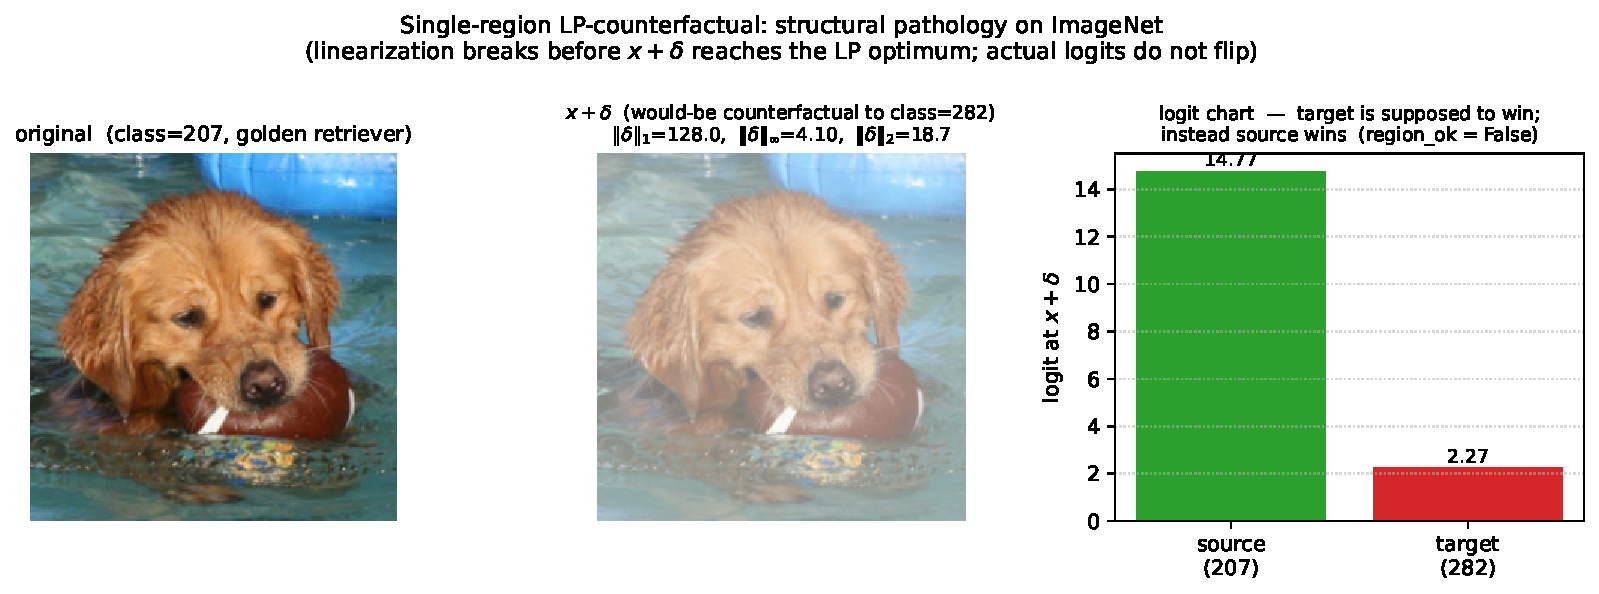
\includegraphics[width=\linewidth]{figures/lp_counterfactual_pathology.pdf}
\caption{Single-region LP-counterfactual structural failure on
DenseNet-121, source class 207 (golden retriever) $\to$ target class
282 (tiger cat). Left: original image $x$. Centre: would-be
counterfactual $x+\delta$ in ImageNet-normalised space ($\delta$
saturates $\sim25$ pixels at their per-channel pixel-space cap). Right:
at the actual (un-clamped) $x+\delta$ the source class still wins by a
large margin ($14.33$ vs.\ $1.14$); \emph{region\_ok = False}: the
region the LP solved against does not contain $x+\delta$. Every one of the
$54$ source/target pairs across the three architectures fails identically
(\emph{region\_ok} $=0/54$, Limitation~L3).}
\label{fig:lp-pathology}
\end{figure}

\WARNING{This figure predates the current revision and is the only image the
manuscript includes. Its caption asserts specific quantities --- source class
$207\to$ target $282$, logits $14.33$ vs.\ $1.14$, and ${\sim}25$ saturated
pixels --- which should be verified against the actual LP-counterfactual run
(the $\delta$ and \emph{region\_ok} records behind the $0/54$ result), and the
figure regenerated if the run has changed, before submission.}

\noindent
The LP-counterfactual is a \emph{theoretical} matrix-direction object,
not an adversarial perturbation (its magnitudes are far outside any
standard budget), and we avoid that framing deliberately. The negative
is that the matrix direction does not transfer to the model's actual
logits once it leaves the source region; a multi-region or
continuation-based reformulation is left as future work
(Section~\ref{sec:limitations}, L3).

\subsection{Teleportation drift is measured, never asserted zero}
\label{sec:study3-teleport}

\paragraph{Why it matters.}
The third negative is a claim we are careful \emph{not} to make. The
temptation in Study~1B (Section~\ref{sec:study1b}) is to enter a table zero
for the knowledge-matrix drift on the strength of the invariance theorem.
Resisting that temptation is what keeps the invariance claim of Study~1
defensible: teleportation does not verify invariance here, because its
transform is function-approximate and fails the theorem's hypothesis. We
do not assert a zero, for two reasons that compound. First, by
Theorem~\ref{thm:nogo} there is \emph{no} bound on knowledge-matrix germ
drift from function-space ($C^0$) closeness alone: two networks can be
uniformly arbitrarily close as functions yet have knowledge matrices
arbitrarily far apart at a point. Second, teleportation on
BatchNorm architectures is function-\emph{approximate}, not exact ---
every one of our $100$ teleports exceeds the $10^{-3}$ logit-drift gate
(up to $\sim10^{-1}$ on ResNet-152) because the BN running statistics are
not migrated under the change-of-basis --- so the invariance theorem's
hypothesis simply does not hold, and an asserted zero would be reporting
a number the experiment did not measure.

\paragraph{Reading.}
We therefore report knowledge-matrix drift under teleportation through
the structure of Proposition~\ref{prop:visdrift}: the visible component
is an identity equal to the logit gate and checked per pair, while the
invisible component carries no a~priori bound (Theorem~\ref{thm:nogo})
and is left unestimated here --- its empirical behaviour is exhibited on
adversarial pairs, where the gate is exact, in Study~2. This reports
only what the violated hypothesis permits, rather than asserting a zero
from a theorem whose hypothesis fails. A BN-aware teleportation that
migrates the running statistics would tighten the gate toward exactness
and is the highest-priority follow-up (Section~\ref{sec:limitations},
L1).

\paragraph{Auxiliary visualisations.}
The \texttt{km\_feature\_viz} pipeline additionally produces a
Jacobian-sensitivity heatmap, DeepDream activation-maximisation
\citep{olah2017feature}, and feature-dictionary artefacts from the same
linearisation; these are exploratory uses of $\Weff(x)$ rather than
tests of any claim in this paper, and we provide them only in the
supplementary HTML index
(\texttt{results/km-feature-viz/\_viewable/index.html}).
% §8  Honest negatives
\section{Limitations}
\label{sec:limitations}

We list, in decreasing order of importance for a reader of this paper,
the concrete limitations that the experiments here \emph{do not} resolve.

\paragraph{(L1) Neural teleportation is function-approximate, not function-exact.}
Study~1B (Section~\ref{sec:study1b}) reports that the equivalence
sanity check returns \texttt{argmax preserved $+$ logit drift > 1e-3}
on every one of the 100 teleports across all three architectures. The
maximum logit drift reaches $\sim 10^{-1}$ on ResNet-152 and stays
under $4 \times 10^{-2}$ on DenseNet-121 and GoogLeNet, so the
invariance theorem's hypothesis (an \emph{exact} per-neuron rescaling)
does not hold and no knowledge-matrix table entry may be asserted from
it. The most likely source is that BatchNorm running statistics
($\mu_{\text{run}}, \sigma^2_{\text{run}}$) are not migrated under the
change-of-basis transformation in \texttt{neuralteleportation}'s
\texttt{random\_teleport}. All three architectures use BatchNorm; the
deeper the network, the larger the cumulative drift. Because the
hypothesis fails, we do \emph{not} assert the knowledge-matrix drift to
be zero: we report it through the three-tier structure of
Proposition~\ref{prop:visdrift}, so that the visible component is the
\emph{measured} logit gate (the equality $\|(\M_\tau-\M)\mathbf{1}\| =
\|f_\tau - f\|$, verified per pair) and the invisible component, which
carries no gate bound (Theorem~\ref{thm:nogo}), is not estimated. A
BN-aware extension of \texttt{random\_teleport} that also permutes /
rescales the running statistics under the same change-of-basis matrices
would tighten the gate from $\sim 10^{-2}$ toward $< 10^{-5}$ and make
the comparison sharper; the qualitative conclusion is robust as stated.
We list this as the highest-priority piece of follow-up engineering.

\paragraph{(L2) The cross-architecture study omits the Cui/Murphy controls.}
The cross-architecture comparison of Study~3 (Section~\ref{sec:study4})
is reported \emph{without} the random-network control of
\citet{cui2022deconfounded} or the shuffled-pair control of
\citet{murphy2024debiased} that accompany the same nine measures in the
single-architecture panel of Section~\ref{sec:study1c}: those controls
were not run in the cross-architecture reduce and are pending. The
cross-architecture numbers should therefore be read as establishing
\emph{availability} --- that the fixed-shape knowledge matrix supports an
alignment-free distance where penultimate measures require dimension
matching --- and not as a control-calibrated quality ranking. Running
the two controls on the cross-architecture pairs is mechanical follow-up
that we defer.

\paragraph{(L3) Single-region LP-counterfactual fails on ImageNet.}
Study~3 (Section~\ref{sec:study3}) reports
\emph{region\_ok = 0/54} on the box-constrained LP. The negative result
is itself reportable, but it does close off a narrative path the paper
might otherwise take (``KMs admit a clean adversarial-style
counterfactual''). Two natural extensions: (i) add per-non-linearity
constraints that keep $\delta$ inside the source's linear region (a
much larger LP, likely infeasible for many class pairs on ImageNet but
worth testing on simpler benchmarks); (ii) accept the multi-region
nature and switch to a homotopy / continuation method that traces the
boundary between consecutive linear regions. We do not pursue these
here.

\paragraph{(L4) Study~1A covers ResNet-152 only.}
Permutation invariance is \emph{automatic} for the knowledge matrix ---
a neuron permutation is a quiver isomorphism, and invariance under it
follows by construction (Proposition~\ref{prop:perm}), not from a
separately-earned property. Study~1A is therefore a numerical
\emph{correctness check} of that prediction, not independent evidence,
and the architecture coverage is correspondingly a software limit rather
than a scientific one. The simple post-pool channel permutation in
Study~1A does not compose through DenseNet's dense connectivity (where
channels are produced by implicit concatenation of fixed-slice
contributions from each \texttt{denselayer}) or GoogLeNet's
Inception-block concat structure (where the four parallel branches
contribute distinct channel counts). Study~1B's neural teleportation
(\citealt{armenta2024neural}) operates on a more general
change-of-basis structure that handles both topologies natively, so
DenseNet-121 and GoogLeNet are tested under Study~1B rather than
Study~1A. A concat-aware permutation that extends the 1A correctness
check to all three architectures is straightforward in principle and is
left as future work.

\paragraph{(L5) Procrustes, Bures, and soft-matching benchmarks deferred to the applications companion.}
Section~\ref{sec:study1c} reports a 9-measure panel
(debiased linear CKA, angular CKA, Procrustes shape distance, Bures
similarity, soft-matching, RSA-Spearman, output JSD, Gromov-Wasserstein,
distance correlation) on the same teleportation pairs as
Section~\ref{sec:study1b}, with random-network~\citep{cui2022deconfounded}
and shuffled-pair~\citep{murphy2024debiased} controls, and
Section~\ref{sec:study4} extends the panel to the cross-architecture
setting.
The Procrustes / Bures / soft-matching family of proper metrics on the
orthogonal-quotient shape space~\citep{williams2021generalized,
harvey2023bures, khosla2024soft} and Gromov-Wasserstein
cross-modality comparisons~\citep{memoli2011gromov} merit deeper
benchmarking --- multi-architecture sweeps including transformer
families, the full ReSi protocol~\citep{klabunde2025resi}, and direct
comparison to model stitching~\citep{bansal2021revisiting} --- which we
defer to the separate, unnumbered applications companion.

\paragraph{(L6) CNN-only.}
We cover the residual / dense / inception family triad
(ResNet-152, DenseNet-121, GoogLeNet). The underlying
quiver-representation framework
\citep{armenta2021representation,armenta2022double} applies to
attention-based architectures as well, but the
\texttt{knowledgematrix} library implementation we rely on does not
yet support attention layers. Extension to transformers is library
engineering rather than theory and is left as future work.

\paragraph{(L7) Cross-architecture penultimate metric is confounded.}
In Study~1B we report penultimate-feature drift in
RMS-per-dimension form, $\| h(x) - h(x') \|_2 / \sqrt{D}$, to
allow side-by-side display across architectures with different
penultimate dimensionalities ($D = 2048$ for ResNet-152, $D = 1024$
for DenseNet-121 and GoogLeNet). This metric is not normalised by
$\| h(x) \|_2$, so absolute cross-architecture rankings reflect
each network's penultimate-feature scale as much as its actual
instability under teleportation. Within-architecture comparisons
(train vs.\ test vs.\ random-input drift) remain valid; cross-arch
rankings should be read with the metric caveat. We discuss this in
a footnote in Study~1B.

\paragraph{(L8) The coherence $A$ is a pixel-basis descriptor with underpowered cells.}
The coherence $A = (d_f/d_M)^2$ of Theorem~\ref{thm:pyth} is a geometric
descriptor read against the single-pixel reference line $A=1$, not a
validated statistic tied to any decision-relevant outcome. Two caveats
that belong in the prose rather than only in the table captions. First,
$A$ is \emph{not} invariant under rotation of the input space: it is
tied to the pixel basis, because $d_M$ is the displacement of $\M(x)$
measured coordinate-wise, so the same pair of inputs viewed in a rotated
input frame would give a different $A$. The reference lines ($A=1$,
$A\le d$) are basis-independent statements about the geometry, but the
per-attack \emph{magnitudes} carry the pixel basis with them. Second,
the per-pair medians are read off uneven and sometimes small samples:
each cell holds $200$ nominal pairs of which $110$--$200$ are valid (FGSM and
PGD keep all $200$; the CW, DeepFool, APGD and Square cells keep $110$--$161$
on every network but VGG, so those entries are low-$n$), and the per-pair median is
exact only for odd valid-pair counts --- only $9$ of $36$ cells have odd
counts, so the even-count cells (the DenseNet-121 column in particular)
are interpolation-approximate. Third, the magnitudes are sensitive to the
filtering convention: on the three cells that retain per-pair records
(VGG/APGD, VGG/DeepFool, VGG/Square) replacing the division guard by the
stricter attack-success filter moves the median $d_M/d_f$ by $-12\%$ to
$-39\%$, and VGG/APGD crosses the $A=1$ line. The Kendall-$W$ attack-family
ordering is a separate, standalone finding and does not inherit the
sample-size or basis caveats; it is not wholly free of the filter caveat
either, since that same recut reorders VGG's top two (CW ahead of
DeepFool), though the family-level grouping --- the level at which we state
the finding --- survives it on every rater we can test. The per-cell
coherence magnitudes inherit all three.

\paragraph{(L9) Fixed pretrained networks only.}
All comparisons here are between fixed pretrained networks; population
statistics across training runs, seed-to-seed baselines and trajectories
are out of scope and are treated in HAaNE~II.
         % §9  Limitations
\section{Conclusion}
\label{sec:conclusion}

\paragraph{Summary.}
We have presented three studies of pretrained ImageNet networks that,
together with two honest negatives, witness a single thesis: the
knowledge matrix is a \emph{canonical arrangement} of a trained network's
per-sample behaviour that penultimate-layer activations cannot supply.
Study~1 (Section~\ref{sec:study1}) is a correctness-and-measurement
study. Its permutation arm verifies the permutation invariance of
Proposition~\ref{prop:perm} on ResNet-152 --- where invariance is automatic
by construction, so this is a numerical correctness check rather than
independent evidence (the load-bearing, non-automatic invariance of
Theorem~\ref{thm:maxinv} is the cross-architecture case): measured signal-relative, random neuron
permutations leave the knowledge matrix with a permutation drift of only
$0.1$--$0.2\%$ of its own adversarial-pair signal (the residual being
float32 accumulation, $\sim10^{-10}$ at float64), while the penultimate
features move by an amount of the same order as their own adversarial
signal. Its teleportation arm measures, rather than asserts, the
knowledge-matrix drift across all three architectures (ResNet-152,
DenseNet-121, GoogLeNet): teleportation visibly perturbs the penultimate
features on every architecture (the similarity panel of
Section~\ref{sec:study1}), while the knowledge matrix does not: the transform is
an exact isomorphism, batch normalisation included, and the matrix's drift under
it is measured at $0.8$--$2.5\times10^{-15}$ relative --- the double-precision
floor --- on all three architectures (Appendix~\ref{app:teleport-exact}).
Study~2 (Section~\ref{sec:study2}) is descriptive geometry: it applies
the visible/invisible decomposition of Theorem~\ref{thm:pyth} to
adversarial pairs and reads the resulting coherence $A=(d_\Psi/d_M)^2$
against the single-pixel line $A=1$. On the deep ImageNet trio every
attack family moves the germ with median $A\le0.23$, well below that
line, and the attack-family ordering of $A$ is stable across six
rater architectures (Kendall $W=0.921$), the population-matched full-scale
appendix panel reproducing the same family-level grouping on all three of
its architectures (Table~\ref{tab:s3_ordering_panel}). Study~3
(Section~\ref{sec:study4}) is an availability result: the fixed-shape
knowledge matrix lets one compare architectures directly, with no
alignment step. The two honest negatives (Section~\ref{sec:study3}) are
the detector bake-off, in which penultimate features win $5$ of $6$
configurations and the original detection claim is withdrawn, and an
LP-counterfactual that fails structurally on pretrained ImageNet networks
(\texttt{region\_ok} = 0/54, Limitation L4).

\paragraph{The umbrella thesis, restated.}
Hidden activations are gauge-covariant and germ-incomplete
(Theorem~\ref{thm:complete}): they change under
network isomorphisms that preserve the function exactly, and they
admit no exact accounting that ties their displacement to the change
in the network's output. The knowledge matrix avoids both: it is an
invariant of the function (Theorem~\ref{thm:maxinv}), and every
displacement splits exactly into a logit-visible and a logit-invisible
part whose balance is the unit-free coherence $A$
(Theorem~\ref{thm:pyth}). For the piecewise-linear networks studied
here, these function-level properties --- invariance and the exact
completeness identity --- are shared with per-class gradient$\times$input
plus an aggregate bias attribution (Theorem~\ref{thm:weff}); what the
knowledge matrix contributes is the canonical \emph{arrangement} of that
data, which is what makes the alignment-free cross-architecture
comparison possible and what the $C$-VJP computation of
Appendix~\ref{app:engineering} exploits. The three studies above, with
their two negatives, are the first witnesses of this thesis.

\paragraph{HAaNE~I is foundational; HAaNE~II asks a different question.}
This paper is HAaNE~I of an ongoing series, and its standalone
contribution is deliberately foundational: a canonical per-sample object,
a characterisation of \emph{exactly} which transformations leave it
invariant (the full function-stabiliser, Theorem~\ref{thm:maxinv}, of
which neuron permutation is one special case), and the resulting
alignment-free cross-architecture comparison that penultimate features
cannot support. We make no application claim in this paper; the
applications that motivated the original framing belong to a separate,
unnumbered companion. Whether independently trained networks share the
knowledge matrix, and how that depends on training, is the subject of
HAaNE~II.

\paragraph{Future directions.}
Subsequent installments take up different questions about the same
object. The next paper, HAaNE~II, asks whether independently trained
networks learn the same knowledge matrix, and how the answer depends on
width, learning rate and parameterisation. Several concrete follow-ups
suggest themselves from the Limitations of this paper. Constructing two
genuinely different architectures that realise the same function on a
neighbourhood --- by dead-unit insertion, neuron splitting, or a width-changing
re-encoding --- and checking that their knowledge matrices agree would supply the
transform-based evidence for cross-architecture invariance that no
same-architecture symmetry can give (closes L1).
A multi-region or continuation reformulation of the
$\M(x)$-counterfactual would convert the structural negative of
Section~\ref{sec:study3} into a positive one (closes L4). Concrete
experiments demonstrating the practical consequences of the
canonical-arrangement claim --- federated-learning aggregation in matrix
space, model comparison without CKA-style alignment, $k$-nearest-neighbour
classification on knowledge matrices --- are the natural application track
of the separate, unnumbered companion (closes L5). Cross-pollination with
transformer-interpretability methods --- training sparse autoencoders on
knowledge-matrix rows
\citep{bricken2023monosemanticity,templeton2024scaling}, projecting
through partial row sums in analogy with the logit lens
\citep{nostalgebraist2020logitlens} --- would extend the framework
beyond the CNN setting of this paper (closes L6).

\paragraph{Closing.}
Hidden activations are not enough. A trained network's behaviour
on a sample is a property of its \emph{function}, and --- unlike the
penultimate activations --- the knowledge matrix derived from its
quiver representation is an invariant of that function
(Theorem~\ref{thm:maxinv}) with an exact accounting of how it moves.
The studies in this paper are the first three
witnesses in a longer multi-witness argument.
          % §10 Conclusion

% ===== Appendices (one file per appendix) =====
\appendix
% ============================================================================
% Proofs appendix for sections section_germ.tex (§2) and section_geometry.tex (§3).
% Same environment
% requirements. Numbering: statements are restated with \ref to the main text.
% ============================================================================

\section{Proofs}
\label{app:proofs}

\paragraph{Verification protocol.} Every identity proved below was also
verified numerically at float64 by two independent adversarial verification
agents with separately written code (including an independent implementation
of the segment traversal for Theorem~\ref{thm:anatomy}); worst-case measured
errors are quoted where informative. Scripts and outputs accompany the
submission package.

\subsection{Preliminaries}

\begin{clarifybox}
\textbf{The vocabulary of this lemma, spelled out.} Fix a network satisfying
(LCS), so that by Proposition~\ref{prop:lcs}(ii) each activation has the form
$f(z)=a_+\max(z,0)+a_-\min(z,0)$.

\emph{Pattern, and $\sigma$.} The \emph{pattern} at $x$ is the assignment to
each hidden unit $(\ell,q)$ of the side of the origin its pre-activation falls
on, equivalently of which of the two slopes $a_\pm$ its entry of $D^{(\ell)}(x)$
takes. It is a vector of bits, one per hidden unit --- for ReLU exactly the
familiar $0/1$ mask. A \emph{candidate} pattern is written $\sigma$: any one of
the $2^{\#\mathrm{units}}$ bit assignments, whether or not some input realises
it. There are finitely many, which is what makes the union below finite.

\emph{Where the activation ``breaks''.} A \emph{breakpoint} of $f$ is a point
where its slope changes, i.e.\ where the two linear pieces meet. Under (LCS)
the only breakpoint is $z=0$ (Proposition~\ref{prop:lcs}(ii)): away from $z=0$
the function is linear and $D$ is locally constant, so the only way a unit's
entry of $D$ can change is for its pre-activation to cross zero. ``The
activation breaks at $z=0$'' means exactly this.

\emph{Frozen pre-activations $z^{(\ell)}_{\sigma,q}$.} Fix $\sigma$ and pretend
every unit below layer $\ell$ has the slope $\sigma$ prescribes, regardless of
the input. Every layer below $\ell$ is then a fixed linear map followed by
multiplication by a fixed diagonal, so the composite is affine and
$z^{(\ell)}_{\sigma,q}(x)=\alpha^\top x+\beta$ for some $\alpha\in\R^d$,
$\beta\in\R$. This is a polynomial of degree at most $1$, and it is
\emph{affine}, not homogeneous: $\beta\neq0$ in general, because the biases
contribute to it. It agrees with the network's realised pre-activation exactly
on the inputs whose pattern below $\ell$ is $\sigma$.

\emph{Zero set, and affine hyperplane.} The \emph{zero set} of
$z^{(\ell)}_{\sigma,q}$ is $\{x\in\R^d: \alpha^\top x+\beta=0\}$ --- the zeros
of that degree-$1$ polynomial, and nothing to do with higher-degree varieties.
When $\alpha\neq0$ this set is an \emph{affine hyperplane}: a translate of a
linear subspace of dimension $d-1$, i.e.\ $\{x:\alpha^\top x=-\beta\}$. It is
closed and Lebesgue-null. When $\alpha=0$ the set is either empty ($\beta\neq0$)
or all of $\R^d$ ($\beta=0$), which is the case the proof handles separately.

\emph{Non-local-constancy set.} A function $g$ is \emph{locally constant at}
$x$ if there is \emph{some} open $U\ni x$ on which $g$ is constant. Its
non-local-constancy set is the set of $x$ where no such $U$ exists. Negating
the quantifiers: $x$ lies in that set iff for \emph{every} open $U\ni x$ there
\emph{exists} $y\in U$ with $g(y)\neq g(x)$ --- the inner quantifier over $y$
is existential, not ``for all''. (Reading it as ``$g(y)\neq g(x)$ for all
$y\in U$'' inverts that quantifier and makes the set look open; it is closed.) We write
$\mathcal B_\ell$ for the non-local-constancy set of the pattern truncated to
layers $1,\dots,\ell$, and $\mathcal B=\mathcal B_L$ for the whole pattern.
\end{clarifybox}

\begin{lemma}[Null switching set]\label{lem:null}
Let $\mathcal B$ be the set of inputs at which the slope diagonal of a network
satisfying (LCS) (Definition~\ref{def:lcs}) is not locally constant --- by
Proposition~\ref{prop:lcs}(ii) the activation breaks only at $z=0$, which is why
the walls below are the zero sets and nothing else. Then $\mathcal B$ is closed and contained in
a finite union of affine hyperplanes; its complement $X_{\mathrm{reg}}$ is
open, dense, and of full Lebesgue measure.
\end{lemma}

\begin{proof}
\emph{$X_{\mathrm{reg}}$ is open, hence $\mathcal B$ is closed.} Let
$x\in X_{\mathrm{reg}}$, so the pattern is constant on some open $U\ni x$. That
same $U$ witnesses local constancy at every one of its points: for $y\in U$ the
set $U$ is an open neighbourhood of $y$ on which the pattern is constant, so
$y\in X_{\mathrm{reg}}$. Hence $U\subseteq X_{\mathrm{reg}}$, and
$X_{\mathrm{reg}}$ is open; $\mathcal B$ is its complement and so is closed.
(The point worth noticing is that one does not construct a new neighbourhood
for each $y$ --- the witness $U$ is reused unchanged.)

\emph{The hyperplane bound.} Induct over layers. For each pattern $\sigma$ and unit
$(\ell,q)$ let $z^{(\ell)}_{\sigma,q}$ be the affine function of $x$ obtained
by freezing the masks below layer $\ell$ to $\sigma$. Let $\mathcal B_{\ell}$
be the non-local-constancy set of the pattern up to layer $\ell$;
$\mathcal B_0=\emptyset$. If $x\notin\mathcal B_{\ell-1}$, the realised
pattern below $\ell$ is constant on a neighbourhood $U$ of $x$, on which the
realised $z^{(\ell)}_q$ equals $z^{(\ell)}_{\sigma,q}$. If
$z^{(\ell)}_{\sigma,q}\equiv0$ then the unit's mask bit is locally constant on
$U$ (an affine function vanishing on an open set vanishes identically, so
there is no partial-vanishing case). Otherwise its zero set is a hyperplane,
off which the bit is locally constant. Hence
$\mathcal B_\ell\subseteq\mathcal B_{\ell-1}\cup\bigcup_{\sigma,q}
\{z^{(\ell)}_{\sigma,q}=0,\ z^{(\ell)}_{\sigma,q}\not\equiv0\}$, a finite
union (patterns that are never realised only enlarge it). For max-pooling, add
the finitely many score-tie hyperplanes.

\emph{Reading off the three conclusions.} Unwinding the induction to
$\ell=L$ puts $\mathcal B=\mathcal B_L$ inside a finite union of sets of the
form $\{z^{(\ell)}_{\sigma,q}=0\}$ with $z^{(\ell)}_{\sigma,q}\not\equiv0$;
each is an affine hyperplane, and the union is finite because there are
finitely many candidate patterns $\sigma$ and finitely many units $q$. That
gives the containment. A hyperplane has Lebesgue measure zero and a finite
union of null sets is null, so $\lambda(\mathcal B)=0$ and
$X_{\mathrm{reg}}=\R^d\setminus\mathcal B$ has full measure. Density follows
from the containment as well: a finite union of hyperplanes has empty interior,
so every ball meets its complement, and $X_{\mathrm{reg}}$ is dense. Openness
was the first paragraph. \qedhere
\end{proof}

\begin{clarifybox}
\textbf{Why this lemma is piecewise-linear and the definition is not.} The
knowledge matrix is defined for \emph{any} activation through the
quotient diagonal \eqref{eq:D-def}, and its row-sum identity needs only that no
pre-activation vanish ($x\in X_{\mathrm{nz}}$) --- nothing about $f(0)$, and
nothing about differentiability. This lemma is a different matter: it is about the set
where the \emph{pattern} is locally constant, and the proof uses that each
$z^{(\ell)}_{\sigma,q}$ is affine, so its zero set is a hyperplane. Both fail
for a strictly nonlinear smooth activation. There $D^{(\ell)}(x)$ takes a
continuum of values and varies continuously with $x$, so the set of inputs with
a locally constant pattern is not of full measure but generically \emph{empty},
and there is no switching set for the lemma to bound. The lemma is therefore
not a technical convenience one could remove by a better definition of
$D^{(\ell)}$: it exists to support the germ identity
(Theorem~\ref{thm:germ}), and it is the germ reading, not the matrix, that is
piecewise-linear in nature. A direct check makes the boundary concrete. At
$x_0=1$ a single $\tanh$ unit with unit weights and the affine map
$x\mapsto f'(1)\,x+\bigl(f(1)-f'(1)\bigr)$ have the \emph{same} germ,
$\bigl(0.419974,\,0.761594\bigr)$, and the same row sum, yet knowledge matrices
$[\,0.761594\mid0\,]$ and $[\,0.419974\mid0.341620\,]$; repeating the
construction with ReLU returns $[\,1\mid0\,]$ for both, as
Theorem~\ref{thm:germ} requires. So for non-PL activations the matrix is not a
function of the germ, and Theorems~\ref{thm:germ}, \ref{thm:maxinv}
and~\ref{thm:complete} are statements about the PL case specifically. Whether
some weaker function-determination survives there is open; we do not claim it.
\end{clarifybox}

\subsection{Proof of Theorem~\ref{thm:germ} (germ identity)}

On a neighbourhood $U$ of $x\in X_{\mathrm{reg}}$ the pattern is constant, so
for every unit $h^{(\ell)}=D^{(\ell)}(x)\,z^{(\ell)}$ on $U$ ($z_q>0$ gives
$\mathrm{ReLU}(z_q)=z_q$; $z_q\le0$ gives $0$). Unrolling,
$\Netxp=\Jwf(x)\,x'+\cwf(x)$ on $U$; differentiate at $x$ and solve for
$c$. For the boundary complement: the same pointwise computation shows
$h^{(\ell)}(x')=D^{(\ell)}(x)\,z^{(\ell)}(x')$ for every $x'$ in the closed
region $\overline{S(x)}$ of $x$'s realised pattern, so the affine map
$A_x(x')=Jx'+c$ agrees with $\Net$ on $\overline{S(x)}$; since $x\in S(x)$
always, $\M(x)\mathbf 1=Jx+c=\Netx$ at every $x$, and for $v$ in the tangent
cone of $S(x)$ at $x$, $\partial^+_v\Net(x)=Jv$ (the one-sided germ from the
inactive side, which is what the convention $\mathbb 1[z>0]$ selects).
\emph{Measured:} probe vs.\ masked product $\le 7\times10^{-15}$; vs.\
finite-difference Jacobian $\le 4\times10^{-11}$; row-sum identity at an
engineered exact-boundary point: $0.0$. \qed

\subsection{Proof of Theorem~\ref{thm:maxinv} (maximal invariance)}

Immediate from Theorem~\ref{thm:germ}: both matrices equal
$[\,D\Net(x)\,\mathrm{diag}(x)\mid \Netx-D\Net(x)x\,]$, a function of the shared germ
alone. The group statement follows because any function-preserving
transformation (any architecture change included) preserves the germ at every
$x\in X_{\mathrm{reg}}$ of both realisations. Sharpness at boundaries: the
identity map and $g(x)=\mathrm{ReLU}(x-1)-\mathrm{ReLU}(1-x)+1\equiv x$
realise the same function, yet at the kink $x=1$ the conventions give
$\M_{\mathrm{id}}(1)=[\,1\mid0\,]$ and $\M_g(1)=[\,0\mid1\,]$ (equal row
sums). \qed

\subsection{Proof of Lemma~\ref{lem:quiver-inv} (quiver-isomorphism invariance) and Proposition~\ref{prop:perm} (permutation scope)}

A quiver isomorphism factors into a per-layer neuron permutation $P_\ell$ and a
positive-diagonal rescaling $T_\ell$ on each hidden layer; we treat the two
generators and compose.

\emph{Permutations.} Let $P_\ell$ permute hidden layer $\ell$, with
$W^{(1)}\!\to P_1W^{(1)}$, $b^{(\ell)}\!\to P_\ell b^{(\ell)}$,
$W^{(\ell)}\!\to P_\ell W^{(\ell)}P_{\ell-1}^{\top}$,
$W^{(L)}\!\to W^{(L)}P_{L-1}^{\top}$, and neuron-wise activations carried with
the units. By induction $z^{(\ell)}(W^{\pi},x)=P_\ell z^{(\ell)}(W,x)$
for every $x$, so the diagonal secant matrices satisfy
$A^{(\ell)}_{\pi}(x)=P_\ell A^{(\ell)}(x)P_\ell^{\top}$ (entrywise ratios
permute; the $0/0\to0$ guard is applied entrywise, hence equivariantly ---
this is where non-equivariant \emph{vector} activations are excluded). The
slope product and the bias accumulation then telescope:
$W^{(L)}P_{L-1}^{\top}\cdot P_{L-1}A^{(L-1)}P_{L-1}^{\top}\cdot
P_{L-1}W^{(L-1)}P_{L-2}^{\top}\cdots=W^{(L)}A^{(L-1)}W^{(L-1)}\cdots$, so
$\KMarg{W^\pi}{x}=\KMwfx$.

\emph{Positive rescalings.} For $T_\ell=\mathrm{diag}(\tau^{(\ell)})$ with
$\tau^{(\ell)}_q>0$, conjugate $W^{(\ell)}\!\to T_\ell W^{(\ell)}T_{\ell-1}^{-1}$,
$b^{(\ell)}\!\to T_\ell b^{(\ell)}$, with the per-neuron activation rescaled to
$\varphi_{\tau}(z)=\tau\,\varphi(z/\tau)$ (for ReLU, $\varphi_\tau=\varphi$).
Then $z^{(\ell)}\!\to T_\ell z^{(\ell)}$ and
$A^{(\ell)}_{\tau}(x)=T_\ell A^{(\ell)}(x)T_\ell^{-1}$, so the inserted factors
$T_\ell^{-1}T_\ell=I$ telescope by the identical argument and
$\KMarg{W^\tau}{x}=\KMwfx$. Composing the two generators gives the lemma.
This recovers the ReLU case of Thms.~4.1--4.2 of the original version.

\emph{Permutation scope (Proposition~\ref{prop:perm}).} The proposition is the
permutation case above, so invariance is immediate; the content is the scope.
The telescoping used that $P_\ell$ commutes with $\varphi$ applied
neuron-wise, which requires elementwise (equivariant) activations; non-equivariant
vector activations break the equivariance of the secant guard above. Moreover,
for activations with $\varphi(0)\neq0$ the row-sum identity itself can fail at
exact $z=0$ points (by $a_q\varphi(0)$; measured example $0.5$), because $P$ no
longer commutes with the constant offset there: a measure-zero caveat the
implementation should carry.
\emph{Measured:} drift $0.0$ at generic and at engineered boundary points,
ReLU and GELU-secant. \qed

\subsection{Proof of Theorem~\ref{thm:complete} (completeness)}

\emph{(i)} $J_{:,i}=\M_{:,i}/x_i$ for $x_i\neq0$ and $c=\M_{:,d+1}$.
\emph{(ii)} $\Net=\M\mathbf 1$ pointwise gives determination on any set; on a
full-measure set, density plus continuity of $\Net$ extends it globally. The germ
at $x$ extends $\Net$ to $\overline{S(x)}$ (proof of Theorem~\ref{thm:germ}),
but no further: $\Psi_1=\mathrm{ReLU}(x-1)$ and $\Psi_3=\mathrm{ReLU}(x)$ have
identical fields ($\equiv[\,0\mid0\,]$) on $(-1,0)$ yet differ at $0.75$ ---
so a field on an open set does not determine $\Net$ even on the region closures
of \emph{other} candidate networks.
\emph{(iii)} For $\tau_q>0$ per hidden unit with weights conjugated,
$z^{(\ell)}\mapsto T_\ell z^{(\ell)}$ and ReLU commutes with positive scalars,
so $a_v\mapsto\tau_v a_v$ while $\Net$ is unchanged.
\emph{(iv)} Write $J=\sum_q D^{(1)}_{qq}\,U_{:,q}\,w_q^{\top}$ with
$U=W^{(L)}D^{(L-1)}\cdots W^{(2)}$. Since $D\Net(x)=J\neq0$, some first-layer
unit $q$ is active with $u:=U_{:,q}\neq0$. Perturb $w_q'=w_q+t e_i$,
$b_q'=b_q-t x_i$: then $z_q'(x)=z_q(x)$ \emph{algebraically}, every hidden
activation at $x$ and $\Netx$ are unchanged, all masks at $x$ are unchanged and
strict (so $x$ stays regular), while the germ moves by the exact rank-one
update $J'-J=u\,(te_i)^{\top}\neq0$ and $c'-c=-t x_i u$, preserving
$J'x+c'=Jx+c$. Two affine maps with different linear parts differ off a
hyperplane, hence on every neighbourhood of $x$; and for any $x_i\neq0$,
column $i$ of $\M$ moves by $t\,x_i\,u\neq0$. (One hidden layer is needed; in
the affine case the same compensation changes nothing.)
\emph{Measured:} activation record equal to $4.4\times10^{-16}$ (2\,ulp),
$\Netx$ equal exactly, rank-one identity $4.7\times10^{-17}$, germ change
$1.9\times10^{-4}\neq0$ at $t=10^{-3}$. \qed

\subsection{Proof of Theorem~\ref{thm:weff} (gradient$\times$input $\oplus$ bias; route equivalence)}

The first $d$ columns of $\M(x)$ are $J_{:,i}x_i=(\partial\Net/\partial x_i)\,x_i$
by the germ identity ($J=D\Net$ at regular $x$, Theorem~\ref{thm:germ}), which is
per-class gradient$\times$input; the bias identity below gives the last column.
The three computation routes (masked product (a), probe (b), autograd (c))
agree, as follows.
(a)$=$germ by Theorem~\ref{thm:germ}. (b): the mask-frozen network is the
affine map $x'\mapsto Jx'+c$; for ReLU the secant $h/z$ equals
$\mathbb 1[z>0]$ ($0/z=0$ for $z<0$; $0/0\to0$ by convention), so probing
$x_ie_i$ through its linear part returns column $J_{:,i}x_i$, and the
zero-input pass through its affine part returns $c$. (c): at regular $x$, $\Net$
is differentiable with $D\Net=J$, and the autograd conventions
($\mathrm{ReLU}'(0)=0$, stored pooling argmax) match the frozen masks even on
the null set. The bias identity: $\partial\Net/\partial b^{(\ell)}
=W^{(L)}D^{(L-1)}\cdots D^{(\ell)}$, and unrolling the bias accumulator gives
$c=\sum_\ell(\partial\Net/\partial b^{(\ell)})\,b^{(\ell)}$.
\emph{Measured} (AlexNet, float64, eval mode): library probe vs.\ autograd
germ $3.3\times10^{-17}$ max-abs (relative $1.3\times10^{-15}$); row sums
$3.5\times10^{-17}$; FullGrad bias identity $6.1\times10^{-16}$. The
network must be in evaluation mode: with dropout active, the saving, probe,
and autograd passes sample different masks and the identity fails at
$\sim10^{-2}$. \qed

\subsection{Proof of Proposition~\ref{prop:contraction} (contraction gap)}

Take the $1$--$2$--$1$ bias-free pair $A$: $w=(1,2)$, $a=(1,1)$ and $B$:
$w=(1,2)$, $a=(1.5,0.75)$. Both realise $\Netx=3\,\mathrm{ReLU}(x)$, so
$\M_A\equiv\M_B$ (measured: $0.0$ on a 401-point grid including the kink). The
per-unit path values $a_qw_q$ are $\{1,2\}$ vs.\ $\{1.5,1.5\}$; any
isomorphism rescales $(w_q,a_q)\mapsto(\tau_qw_q,a_q/\tau_q)$, preserving each
$a_qw_q$, and permutations permute the multiset --- since the multisets
differ, the networks are non-isomorphic and the path-resolved representations
differ at every $x>0$. The identifiability statement on the
\citet{phuong2020functional} class follows by chaining $\Net=\M\mathbf 1$
(field determines the function on a full-measure subset of their domain $Z$,
hence on $Z$ by continuity) with their Theorem~1, quantifiers intact: there
exists $W^{*}$ such that any \emph{general} network of the \emph{same
architecture} agreeing with it on $Z$ is permutation$\times$positive-rescaling
equivalent; the converse direction is Proposition~\ref{prop:perm} plus
rescaling invariance. (Note the $1$--$2$--$1$ example has increasing widths,
consistently outside their architecture class.) \qed

\subsection{Proof of Theorem~\ref{thm:pyth} (visible/invisible decomposition)}

For any $a\in\R^C$ and any $Q'$ with $Q'\mathbf 1=0$:
$\langle a\mathbf 1^{\top},Q'\rangle_F=a^{\top}(Q'\mathbf 1)=0$, so
$\mathcal V=\{a\mathbf 1^{\top}\}$ and $\mathcal N=\{Q:Q\mathbf 1=0\}$ are
orthogonal complements; $A\mapsto(A\mathbf 1)\mathbf 1^{\top}/(d{+}1)$ is the
orthogonal projector onto $\mathcal V$. With
$P=\Delta\Net\,\mathbf 1^{\top}/(d{+}1)$:
$P\mathbf 1=\Delta\Net$, $Q=\Delta\M-P\in\mathcal N$, and
$\|P\|_F^2=\|\Delta\Net\|^2/(d{+}1)$, giving the Pythagorean identity. The
constraint set $\{A:A\mathbf 1=\Delta\Net\}$ is $P+\mathcal N$, so $P$ is its
unique minimum-norm element; equality in the floor iff $Q=0$, i.e.\ constant
rows (per row, Cauchy--Schwarz against $\mathbf 1$). Monotonicity of
$t\mapsto1/\sqrt{(d{+}1)t}$ gives the rank-statistic correspondence (for
medians of even-count samples the interpolated median commutes only up to the
gap between the central order statistics --- below quoting precision in our
tables). Invariances: output rescaling and gauge invariance are immediate from
invariance of $\M$ and linearity; for $x\mapsto Sx$,
$W^{(1)}\mapsto W^{(1)}S^{-1}$ (diagonal $S$): $J\mapsto JS^{-1}$ and
$\mathrm{diag}(Sx)=S\,\mathrm{diag}(x)$, so $J\,\mathrm{diag}(x)$ is
unchanged. Non-invariance under rotations is exhibited numerically (function
preserved to $1.8\times10^{-15}$, $d_M$ changed by up to $57\%$).
\emph{Measured:} identities $\le1.7\times10^{-15}$ over $2{,}400$ random
instances; min-norm never beaten in $10^4$ trials. \qed

\subsection{Proof of Theorem~\ref{thm:within} (within-region anatomy)}

Same strict pattern at $x$ and $y$ puts the segment in one convex region with
common $(J,c)$, so $\M(y)-\M(x)=[\,J\,\mathrm{diag}(y)-J\,\mathrm{diag}(x)
\mid c-c\,]=[\,J\,\mathrm{diag}(\delta)\mid0\,]$ and the column-energy formula
follows. (i): with $a_i=\delta_iJ_{:,i}$,
$\|\sum_ia_i\|^2\le(\sum_i\|a_i\|)^2\le d\sum_i\|a_i\|^2$ (triangle, then
Cauchy--Schwarz), equality iff all $a_i$ equal and nonzero --- attained by
$J=u\mathbf 1_d^{\top}$, $\delta=\mathbf 1_d$. (ii): a single nonzero column
$a=s\,J_{:,i_0}$ gives $d_M=\|a\|=d_\Psi$ and exactly one nonzero column with a
zero bias column. (iii): at most $k$ nonzero columns; the same
Cauchy--Schwarz over the support gives $A\le k$ and the participation bound.
\emph{Measured:} closed form $\le5\times10^{-13}$; cap never violated
($2\times10^4$ trials); one-pixel law exact; $A=1+5.5\times10^{-10}$ in the
finite-step demo. \qed

\subsection{Proof of Theorem~\ref{thm:anatomy} (smooth $+$ crossing)}

\emph{Dyad lemma.} At a transversal single flip of unit $k$ in layer
$\ell^{*}$ at point $z$ on the segment, with $\sigma=\pm1$ the mask change,
the region data jump by $J_{+}-J_{-}=\sigma\,u_kv_k^{\top}$ and
$c_{+}-c_{-}=\sigma\,\gamma_ku_k$, where
$u_k=U^{(\ell^{*}+1)}W^{(\ell^{*}+1)}e_k$,
$v_k^{\top}=e_k^{\top}W^{(\ell^{*})}L^{(\ell^{*})}$, and
$z^{(\ell^{*})}_k(x')=v_k^{\top}x'+\gamma_k$; continuity of $\Net$ across the
wall forces the bias jump, and $v_k^{\top}z+\gamma_k=0$ at the crossing makes
the full dyad's row sums vanish:
$\sigma u_k(v_k^{\top}z+\gamma_k)=0$.
\clarify{Here $U^{(\ell^{*}+1)}$ and $L^{(\ell^{*})}$ denote the downstream and
upstream masked products of the region data shared by the two sides of the
wall, i.e.\ $U^{(\ell^{*}+1)}=W^{(L)}D^{(L-1)}\cdots D^{(\ell^{*}+1)}$ and
$L^{(\ell^{*})}=D^{(\ell^{*}-1)}W^{(\ell^{*}-1)}\cdots D^{(1)}W^{(1)}$ in the
factorisation $J=W^{(L)}D^{(L-1)}\cdots D^{(1)}W^{(1)}$ of
Section~\ref{sec:germ}; so $u_k\in\R^{C}$ is unit $k$'s output-side vector,
$v_k\in\R^{d}$ its input-side vector, and $\gamma_k$ the bias accumulated in
its pre-activation.}

\emph{Telescope.} Write
$\M(y)-\M(x)=\sum_{j=0}^{N}\bigl[\M^{(j)}(z_{j+1})-\M^{(j)}(z_j)\bigr]
+\sum_{j=1}^{N}\bigl[\M^{(j)}(z_j)-\M^{(j-1)}(z_j)\bigr]$, where
$\M^{(j)}(z)=[\,J_j\,\mathrm{diag}(z)\mid c_j\,]$ is the $j$-th region's
matrix evaluated at $z$ (well defined on closures). Each smooth term is
$[\,J_j\,\mathrm{diag}((t_{j+1}-t_j)\delta)\mid0\,]$ by
Theorem~\ref{thm:within}; summing gives $\bar J$. Each jump term is a dyad of
the lemma. Row sums: the smooth part gives $\bar J\delta$, the dyads give $0$,
and $\Nety-\Netx=\int_0^1J(x+t\delta)\,\delta\,dt=\bar J\delta$ by the
fundamental theorem of calculus for the PL map on the segment. The bias
column of the smooth part is zero, so the bias column of $\M(y)-\M(x)$ is
exactly $c(y)-c(x)=\sum_j\sigma_j\gamma_{k_j}u_{k_j}$ --- equivalently, it is
constant on chambers of pair space with fixed crossing combinatorics, which is
the soundness direction of the crossing detector (no crossings $\Rightarrow$
zero bias column). The converse fails: bias-free networks have all
$\gamma_k=0$ (measured: $19$ crossings, bias column exactly $0$), a flipped
unit cut off downstream has $u_k=0$, and multi-crossing cancellations exist.
Genericity (finitely many transversal single crossings) holds off a null set
of pairs by a routine transversality argument over the finite wall complex,
assuming no two units share a wall piece --- exactly duplicated units in
pruned or weight-tied networks violate it and should be screened.
\emph{Hamming.} A unit whose endpoint mask bits differ flips an odd number of
times ($\ge1$); equal bits flip an even number ($\ge0$): $H\le N_{\mathrm{cross}}$
with parity equality, and equality iff no unit flips twice (first-layer walls
are flat, so first-layer units never flip back along a segment; deeper walls
are bent and do --- measured: a hat-shaped network with $N=4$, $H=2$).
\emph{Measured:} full decomposition $\le2.6\times10^{-16}$ over $>1{,}000$
crossings with two independent traversal implementations; bias-column formula
$\le8.2\times10^{-13}$. \qed

\subsection{Proof of Proposition~\ref{prop:dichotomy}}

On the gauge orbit of $W$ (positive rescalings), $\Net$, $d_\Psi$, and $d_M$
are fixed (invariance of $\Net$ and of $\M$), while the penultimate distance
$d_h$ between a fixed pair's features sweeps an unbounded range (rescale one
penultimate unit by $\lambda$: measured $d_h\in[0.44,\,15.3]$ with $\Net$
bitwise fixed). Hence any gauge-invariant function of the stored statistics
$(d_h,d_\Psi)$ is constant in $d_h$ on orbits, i.e.\ uses no penultimate
information. The KM accounting exists because the constraint
$\M\mathbf 1=\Net$ pairs all matrices against the \emph{fixed} vector
$\mathbf 1$; the last-layer relation $\Delta\Net=W^{(L)}\Delta h$ pairs features
against a parameter-dependent map, whose induced ``visible fraction''
$1/(1+\lambda^2)$ in the worked example takes every value in $(0,1)$ across
one orbit. \qed

\subsection{Proof of Theorem~\ref{thm:nogo} and Proposition~\ref{prop:visdrift}}

\emph{No-go.} In $d=C=1$ take
$g(t)=K\,\mathrm{ReLU}(t-x_0)-K\,\mathrm{ReLU}(t-x_0-\varepsilon/K)$ and
$\Net\equiv0$ realised with the same first layer and zeroed second layer. Then
$\sup_t|\Psi-g|=\varepsilon$ exactly; at $x=x_0+\varepsilon/(2K)$ both networks
have masks $(1,0)$; but $J_g(x)=K$, $J_\Psi(x)=0$, so
$\|\M_g(x)-\M_\Psi(x)\|_F=K\sqrt{x^2+x_0^2}\to\infty$ as $K\to\infty$ at fixed
$\varepsilon$ (the construction needs the ramp away from the origin,
$x_0\neq0$). \emph{Measured:} drift $1.4\times10^{2},10^{4},10^{6}$ at
$K=10^{2},10^{4},10^{6}$, $\varepsilon=10^{-2}$ fixed.
\emph{Visible bound.} $\|(\M_\tau(x)-\M(x))\mathbf 1\|=\|\Psi_\tau(W\!,f)(x)-\Netx\|$ is
the row-sum identity; the projection onto constant-row matrices then has norm
$\le\varepsilon/\sqrt{d+1}$. \emph{Conditional bound.} If both networks are
affine on $B(x,r)$ with $\varepsilon_r=\sup_{B(x,r)}\|\Psi_\tau(W\!,f)-\Net\|$, then for
any unit vector $u$, $2r\,\Delta J\,u$ is a difference of differences of
$\Psi_\tau(W\!,f)-\Net$ at $x\pm ru$, so $\|\Delta J\|_{\mathrm{op}}\le\varepsilon_r/r$;
combine $\|\Delta J\,\mathrm{diag}(x)\|_F\le\|x\|_\infty\sqrt{\min(C,d)}\,
\|\Delta J\|_{\mathrm{op}}$ with
$\|\Delta c\|\le\varepsilon_r+\|\Delta J\|_{\mathrm{op}}\|x\|_2$.
\emph{Measured} (exact trust-region computation of $\varepsilon_r$):
$0/120$ violations, minimum slack $0.21$. \qed
      % Appendix A  Proofs
\section{Computing the knowledge matrix}
\label{app:engineering}

This appendix collects all of the software and computational material for the
knowledge matrix, so that the main text can remain conceptual. It states the
three equivalent ways to compute $\M(x)$ that Theorem~\ref{thm:weff}
establishes, gives the cost accounting that motivates the autograd route,
reports the numerical validation that the three routes agree, and lists the
implementation requirements that make the row-sum identity
$\M(x)\mathbf{1}=f(x)$ hold exactly. Throughout, $\M(x)\in\R^{C\times(d+1)}$ is
the knowledge matrix of a feedforward, piecewise-linear (PL) network with $C$
output classes on an input of dimension $d$; its slope block is
$\Weff(x)=J=\partial f/\partial x\in\R^{C\times d}$ and its final column is the
aggregate bias attribution $\beff(x)=f(x)-Jx$.

\subsection{Three equivalent computations}
\label{app:eng-three-routes}

For a PL network at a regular point (one not on a non-linearity's switching
surface), the knowledge matrix can be obtained by three routes that coincide.

\paragraph{(i) Masked product.}
Freeze the activation pattern at $x$: each non-linearity contributes a fixed
diagonal mask $D^{(\ell)}(x)$ recording which units are active. On the resulting
mask-frozen affine map, the slope block is the ordered product
$\Weff(x)=W^{(L)}D^{(L-1)}\cdots D^{(1)}W^{(1)}$, evaluated at $x$, and the bias
column is the corresponding aggregate of the per-layer biases pushed through the
same masks. This is the definitional route used by the
\texttt{knowledgematrix} library probe internally.

\paragraph{(ii) Probe construction ($d{+}1$ forward passes).}
The library realises the masked product without ever forming it explicitly, by
freezing the mask at $x$ and then sending $d{+}1$ scaled basis vectors through
the mask-frozen network: one column of $\M(x)$ per input coordinate (recovering
$\Weff$ column by column) plus one pass for the bias column. This is $d{+}1$
forward passes of the (now affine) network. At ImageNet scale this is the
expensive route, because $d{+}1 = 150{,}529$.

\paragraph{(iii) Autograd ($C$ vector--Jacobian products plus one forward pass).}
Because $\Weff(x)=J=\partial f/\partial x$ is exactly the Jacobian of the
network output with respect to the input at $x$, the slope block can be read off
by automatic differentiation: $C$ vector--Jacobian products (one per output
class, each seeding a unit covector $e_c$) recover the $C$ rows of $J$, and one
additional forward pass gives $f(x)$, from which the bias column is
$\beff(x)=f(x)-Jx$. This is $C$ backward passes plus one forward pass.

By Theorem~\ref{thm:weff} these three routes coincide at almost every input for
PL networks: they agree at every regular point, i.e.\ off the measure-zero set
of switching surfaces. On that null set the gradient is not single-valued and
the probe inherits whichever one-sided pattern the forward pass selects; we
compute at regular points throughout. The equality of (i)--(iii) is what lets us
use the cheapest route, (iii), in practice while retaining the library probe
(ii) as the reference implementation. Per Theorem~\ref{thm:weff}, this slope
block is per-class gradient$\times$input and the bias column is an aggregate bias
attribution in the FullGrad sense
\citep{shrikumar2016not,ancona2018towards,srinivas2019full}; the function-level
properties of $\M$ on PL nets are shared with that data, and what the matrix
contributes is the canonical \emph{arrangement} rather than a separate
invariant.

\subsection{Cost and speed-up}
\label{app:eng-cost}

Theorem~\ref{thm:weff} replaces $d{+}1$ probe passes by $C$ backward passes,
a predicted saving of $\approx(d{+}1)/(\kappa C+1)$, where $\kappa$ is the
forward-to-backward cost ratio. At ImageNet scale ($C=1000$,
$d{+}1=150{,}529$) this is a factor in the $50$--$150\times$ band (JSON key
\texttt{timing\_224.thm\_predicted\_ratio\_range} $=[50.2,\,150.4]$). The demo
below reports a measured CPU ratio of $\approx296\times$, above the theory band
for the reasons noted there; we report it as a compute-cost ratio consistent
with the lower-bound estimate, not as a tighter claim than the theory supports.

\subsection{Numerical validation: $\Weff$ $=$ grad$\times$input, three ways}
\label{app:eng-validation}

This subsection reports the numerical demonstration anchoring
Theorem~\ref{thm:weff}: that the three routes of
Appendix~\ref{app:eng-three-routes} agree to machine precision, and that the
autograd route is cheaper. We expose the bare slope
$\Weff(x)=J=\partial f/\partial x \in \R^{C\times d}$ (the knowledge matrix
$\M(x)$ before its bias column is appended) through the library probe's
\verb|extract_weff=True| flag, and compare it against (a) the masked product
$W^{(L)}D^{(L-1)}\cdots D^{(1)}W^{(1)}$ evaluated at $x$, and (b) autograd
($C$ vector--Jacobian products plus one forward pass). All computations are
in \texttt{float64} with the network in evaluation mode, the conditions under
which the row-sum identity $\M(x)\mathbf{1}=f(x)$ is exact. Per
Theorem~\ref{thm:weff}, every function-level property of $\M$ on PL nets
(invariance, completeness, the exact row sum) is already shared by
gradient$\times$input with an aggregate bias attribution in the FullGrad
sense \citep{shrikumar2016not,ancona2018towards,srinivas2019full}; what the
matrix contributes is the canonical \emph{arrangement}, not a separate
invariant. This subsection only checks that the three routes to that shared
slope coincide, and that the autograd route is cheaper.

\paragraph{Three-route agreement on a small MLP.}
On a tiny MLP at a regular point, the masked product, the probe, and autograd
agree to the float64 floor: probe-vs-product max-abs error
$7.1\times10^{-15}$, autograd-vs-product $3.6\times10^{-14}$, the row-sum
residual $\|\M(x)\mathbf{1}-f(x)\|_\infty = 2.0\times10^{-14}$, and the
$\Weff$ identity $\|[\,\Weff\mid c\,]\,\mathbf{1}-f(x)\|_\infty
= 2.1\times10^{-14}$.
(JSON keys \texttt{mlp\_three\_route\_max\_abs\_err}.\{\texttt{prod\_vs\_probe},
\texttt{prod\_vs\_auto}, \texttt{rowsum}, \texttt{weff\_identity}\}.) As a
sanity check on the geometry of Theorem~\ref{thm:within}, a single-pixel
perturbation on the same network gives $d_M = d_f$ to
$|A-1| = 5.5\times10^{-10}$ with exactly one nonzero column, the one-pixel
law $A=1$ (key \texttt{one\_pixel\_law}).

\paragraph{Probe-vs-autograd agreement on AlexNet.}
The exactness check at scale uses AlexNet on a $3\times64\times64$ input
($d=12{,}288$, $C=1000$; the fork's fully connected dimensions constrain the
input size, so this check is run at $64\times64$, not at the $224\times224$
size used for the timing extrapolation below), with random weights at a
regular point (the identities are parameter-independent). The library probe
and autograd agree to a max-abs error of $3.2\times10^{-17}$ on $\M(x)$ (key
\texttt{M\_lib\_vs\_M\_auto\_max\_abs}; the two reported rows are
$3.21\times10^{-17}$ and $3.30\times10^{-17}$), the bare-slope route
$\Weff$ matches autograd to $\approx 4.8\times10^{-19}$ max-abs (key
\texttt{weff\_vs\_autograd}: $4.8\times10^{-19}$ and $4.1\times10^{-19}$),
and the row-sum residual is $\le 3.5\times10^{-17}$ (probe) and
$\le 1.2\times10^{-17}$ (autograd).

\paragraph{Finite-precision behaviour at depth.}
The float64 agreement above is the favourable case. In \texttt{float32} the
row-sum completeness residual is materially larger on deep networks --- it
reaches $0.15$--$0.30$ on ResNet-152 --- and falls to $\sim10^{-10}$ when the
same computation is repeated at \texttt{float64}. The exact row sum is therefore
a property of the idealised PL map, not of finite arithmetic at depth; we
report completeness as exact in theory and measured-near-exact at float64, and
we do not claim agreement ``to numerical precision'' in single precision.

\paragraph{Compute cost.}
Theorem~\ref{thm:weff} replaces $d{+}1$ probe passes by $C$ backward passes,
a predicted saving of $\approx(d{+}1)/(\kappa C+1)$, i.e.\ a factor in the
$50$--$150\times$ band at ImageNet scale ($C=1000$, $d{+}1=150{,}529$; JSON
key \texttt{timing\_224.thm\_predicted\_ratio\_range} =
$[50.2,\,150.4]$). The demo's measured cost ratio on this hardware is
$\approx296\times$ (probe path $\approx8475$\,s, VJP path $\approx29$\,s per
sample, both extrapolated from measured slices; key
\texttt{ratio\_probe\_over\_vjp}). The measured figure lies above the theory
band because it is an \texttt{float64} CPU run in which the probe passes are
emulated by batched forward evaluations (JSON \texttt{timing\_224.note});
we report it as a compute-cost ratio, consistent with the lower-bound theory
estimate. The smaller AlexNet check confirms the same ordering directly
(probe $\approx23.7$\,s vs.\ VJP $\approx14.7$\,s per sample at $64\times64$).

\subsection{Implementation requirements}
\label{app:eng-gotchas}

The identities above hold for the idealised PL map; reproducing them in software
requires the following.

\paragraph{Evaluation mode is mandatory.}
The network must be in evaluation mode for every pass used to build $\M(x)$.
Active Dropout desynchronises the saving, probe, and autograd passes --- each
draws a different mask --- so the three routes no longer share an activation
pattern, and the row-sum identity $\M(x)\mathbf{1}=f(x)$ then appears to fail at
the $\sim10^{-2}$ level. This is not a violation of Theorem~\ref{thm:weff} but a
mismatch of activation patterns across passes; \texttt{model.eval()} (freezing
Dropout, and BatchNorm to running statistics) removes it.

\paragraph{Input shape.}
The \texttt{KnowledgeMatrixComputer} forward call expects a $3$D input tensor
$(C_{\text{in}},H,W)$, \emph{not} a $4$D batched tensor $(1,C_{\text{in}},H,W)$;
the leading batch axis must not be added with \texttt{unsqueeze} before the
call. (Here $C_{\text{in}}$ is the number of input channels, distinct from the
$C$ output classes that index the rows of $\M$.)

\paragraph{Chunked computation and storage discipline.}
At ImageNet scale a single knowledge matrix is $1000\times150{,}529$, so per-sample
matrices are large and a sweep produces many of them. Computation is chunked, and
matrices are \emph{not} written one file per sample onto shared cluster storage:
the per-sample files are computed on node-local scratch and bundled into a single
archive before being shipped to shared storage, to avoid the metadata load of
many small files on a parallel filesystem. The autograd route of
Appendix~\ref{app:eng-cost} compounds with this: fewer passes per sample and
fewer intermediate writes.
 % Appendix B  Computing the KM in software
%   (anchors thm:weff and the main-text forward pointers \ref{app:engineering})

% Appendix: teleportation exactness. Establishes that neural teleportation is an
% EXACT isomorphism (BatchNorm in eval mode included) and that the drift Study 1B
% measures is floating-point roundoff -- verified by the precision-scaling law
% (fp32/fp64 ratio = eps32/eps64) in scripts/verify_teleportation_exactness.py.
% This supersedes the earlier "function-approximate" reading of Step B.
% ============================================================================
%  Appendix: neural teleportation is an exact isomorphism; the measured logit
%  drift is floating-point roundoff.
%
%  Added 2026-09-07. This appendix REPLACES the earlier "teleportation is
%  function-approximate" diagnosis, which attributed the measured drift to
%  un-migrated BatchNorm running statistics. That diagnosis was a conjecture
%  (docs/Final-twist/km-notes.md, 2026-05-01, "Most likely cause: ...") and it
%  is wrong: the library does not migrate the running statistics because it does
%  not need to. See scripts/verify_teleportation_exactness.py.
% ============================================================================

\section{Neural teleportation is exact: the measured drift is roundoff}
\label{app:teleport-exact}

That neural teleportation preserves the function exactly is a theorem, not a
finding of this paper: an isomorphism of neural networks $\tau:(W,f)\to(V,g)$
satisfies $\Psi(W,f)=\Psi(V,g)$ \citep[Thm.~4.13]{armenta2021representation}, and
a per-neuron change of basis is such an isomorphism. This appendix does two
things that the theorem does not. Section~\ref{app:teleport-why} records why
batch normalisation is inside the theorem's scope rather than an exception to it,
since that is the point at which the construction is most often doubted.
Sections~\ref{app:teleport-eps}--\ref{app:teleport-tf32} then verify that our
\emph{software} realises the identity, and calibrate the arithmetic floor below
which no drift figure in this paper can be resolved --- a question about the
implementation, on which a theorem is silent.

\subsection{Why the transform is exact, batch normalisation included}
\label{app:teleport-why}

A teleportation assigns a nonzero scalar $\tau_q$ to each hidden neuron $q$ and
conjugates the parameters, $W^{(\ell)}\mapsto T_\ell W^{(\ell)}T_{\ell-1}^{-1}$
and $b^{(\ell)}\mapsto T_\ell b^{(\ell)}$ with $T_\ell=\mathrm{diag}(\tau)$. The
group acts on the activations as well, by
\begin{equation}
(\tau\cdot f)_v(z)\;=\;\tau_v\,f_v\!\left(\frac{z}{\tau_v}\right)
\label{eq:cob-activation}
\end{equation}
at each hidden vertex $v$ \citep[Eq.~2]{armenta2021representation}. For a
positively homogeneous activation --- ReLU with $\tau_v>0$ --- this leaves $f_v$
unchanged, the $T_\ell$ telescope through the layer stack, and the function is
preserved.

Batch normalisation is the case that looks like an obstruction, and it is worth
being explicit about why it is not. In evaluation
mode a BN channel is the affine
map $z\mapsto\gamma(z-\mu)/\sqrt{\sigma^2+\epsilon}+\beta$, which is
\emph{not} positively homogeneous: the running mean $\mu$ and the shift $\beta$
break $\varphi(\tau z)=\tau\varphi(z)$. One repair is to migrate the running
statistics, $\mu\mapsto\tau\mu$ and $\sigma^2\mapsto\tau^2\sigma^2$; note that
this repair is only exact if the numerical guard $\epsilon$ is rescaled too,
since $\sqrt{\tau^2\sigma^2+\epsilon}\neq\tau\sqrt{\sigma^2+\epsilon}$.

None of that is necessary, because the framework already prescribes the answer.
Two facts settle it. First, in evaluation mode $\mu$ and $\sigma^2$ are not
batch-dependent quantities but ordinary weights of the network
\citep[Remark~5.4]{armenta2021representation}, so a normalisation layer is a pair
of affine vertices like any other and Theorem~4.13 applies to it unchanged.
Second, the action on its activation is given by
Equation~\eqref{eq:cob-activation}, and that is precisely what the
\texttt{neuralteleportation} implementation computes: it divides the incoming
activation by the incoming change of basis, applies the unmodified
normalisation, and carries the outgoing basis on the affine parameters,
\[
z \;\xrightarrow{\;\text{incoming COB}\;}\; \tau_{\mathrm{in}} z
\;\xrightarrow{\;\div\,\tau_{\mathrm{in}}\;}\; z
\;\xrightarrow{\;\mathrm{BN}_{\mu,\sigma^2,\epsilon}\;}\; \mathrm{BN}(z)
\;\xrightarrow{\;\gamma,\,\beta\;\times\;\tau_{\mathrm{out}}\;}\;
\tau_{\mathrm{out}}\,\mathrm{BN}(z).
\]
which is Equation~\eqref{eq:cob-activation} with $f_v=\mathrm{BN}$. The division
restores the original pre-normalisation activation exactly, so the original
$\mu$, $\sigma^2$ and $\epsilon$ remain correct, and the composite is
$\tau_{\mathrm{out}}\mathrm{BN}(z)$ --- with no condition on $\epsilon$, and no
migration of the running statistics. Teleportation of a batch-normalised network
in evaluation mode is therefore function-exact, and satisfies the hypotheses of
Theorem~\ref{thm:maxinv} and Lemma~\ref{lem:quiver-inv} exactly.

We note one boundary of the framework that bears on this paper elsewhere:
\citet{armenta2021representation} observe that average and global-average pooling
sit inside it without qualification, whereas max-pooling ``break[s] the algebraic
structure'' --- the same tie-dependence that Theorem~\ref{thm:weff} excludes by
hypothesis.

\subsection{The measured drift scales with machine epsilon}
\label{app:teleport-eps}

Exactness in real arithmetic does not mean a zero measurement in floating point.
The round trip above --- multiply by $\tau_{\mathrm{in}}$ inside the preceding
convolution, then divide by $\tau_{\mathrm{in}}$ inside the normalisation --- is
exact over $\R$ but not over floats: the convolution is recomputed with rescaled
weights, so its partial sums have different magnitudes and round differently.
The drift is therefore $O(\varepsilon_{\mathrm{mach}})$ and, decisively,
\emph{linear in the working precision}.

That is a falsifiable prediction, and it separates the two hypotheses cleanly. If
the transform genuinely changed the function --- if the running statistics really
were stale --- the discrepancy would be a property of the weights and would be
essentially \emph{independent} of working precision, giving a
\texttt{fp32}/\texttt{fp64} ratio near $1$. If it is roundoff, the ratio must be
near $\varepsilon_{32}/\varepsilon_{64}=2^{29}\approx5.4\times10^{8}$.

We ran the identical change-of-basis draw (same seed, same COB vector) at both
precisions on all three architectures, with the library's three internal
\texttt{float32} down-casts patched out so that the \texttt{fp64} arm is
genuinely double precision.\footnote{The library hard-casts to single precision
in \texttt{COBForwardMixin.forward}, in \texttt{layers/merge.py:Add.forward} (the
residual skip connection), and via a \texttt{float32} tracing input in
\texttt{NeuralTeleportationModel.\_\_init\_\_}. Without these three patches the
\texttt{fp64} arm silently retains a single-precision floor and the ratio
saturates near $10$.} Table~\ref{tab:teleport-exactness} reports the result.

\begin{table}[t]\centering\small
\caption{Teleportation is exact; the drift is roundoff. Maximum absolute logit
discrepancy $\max|\Net-\Psi_\tau(W\!,f)|$ between a network and its teleported image, for the
\emph{same} change-of-basis draw evaluated at two working precisions ($5$ seeds,
$8$ inputs, \texttt{cob\_range}$=1$, CPU, evaluation mode). The \texttt{fp64}
discrepancy sits at the double-precision floor ($\sim10^{-15}$ relative), and the
ratio between the two columns matches
$\varepsilon_{32}/\varepsilon_{64}=5.37\times10^{8}$ --- the signature of pure
roundoff. A genuine change of function would give a ratio near $1$.}
\label{tab:teleport-exactness}
\smallskip
\begin{tabular}{@{}lccc@{}}\toprule
Architecture & \texttt{fp32} drift & \texttt{fp64} drift (relative) & \texttt{fp32}/\texttt{fp64} ratio \\ \midrule
ResNet-152   & $4.2$--$6.1\times10^{-6}$ & $8.2\times10^{-15}$--$1.0\times10^{-14}$ \; ($1.4$--$1.7\times10^{-15}$) & $4.2$--$6.7\times10^{8}$ \\
DenseNet-121 & $6.2$--$10.5\times10^{-6}$ & $1.2$--$2.3\times10^{-14}$ \; ($1.6$--$3.2\times10^{-15}$) & $3.3$--$7.9\times10^{8}$ \\
GoogLeNet    & $5.7$--$8.6\times10^{-6}$ & $1.4$--$1.7\times10^{-14}$ \; ($1.9$--$2.2\times10^{-15}$) & $3.4$--$5.7\times10^{8}$ \\
\bottomrule\end{tabular}\end{table}

The ratio is $3.3$--$7.9\times10^{8}$ across all fifteen runs, straddling the
predicted $5.37\times10^{8}$; the \texttt{fp64} residual is $1.4$--$3.2\times
10^{-15}$ relative, i.e.\ at the double-precision floor. The measured drift is
roundoff, and nothing else.

\subsection{The knowledge matrix itself, not merely the logits}
\label{app:teleport-km}

The logit test above certifies that the \emph{function} is preserved. The
knowledge matrix is a strictly finer object --- it records the germ, which
Theorem~\ref{thm:nogo} shows the logits do not control --- so it deserves its own
check. Writing $\Psi_c$ for class $c$'s component of $\Net$, we recomputed
knowledge-matrix rows directly, as
$\M_{c,:}(x)=[\,\nabla_x\Psi_c(x)\odot x \mid \Psi_c(x)-\nabla_x\Psi_c(x)^{\!\top}x\,]$
by one vector--Jacobian product per class, for the original and the teleported
network, at both precisions ($12$ class rows, \texttt{cob\_range}$=1$).

At double precision the knowledge-matrix drift is
$0.8$--$2.5\times10^{-15}$ relative across all six runs --- the same
machine-epsilon floor as the logits. \emph{The knowledge matrix is invariant under teleportation to double
precision}, on ResNet-152, DenseNet-121 and GoogLeNet alike, exactly as
Lemma~\ref{lem:quiver-inv} requires.

Two scope notes, so this test is not read for more than it establishes. First,
the bias column here is \emph{derived} as $\Psi_c(x)-\nabla_x\Psi_c(x)^{\!\top}x$
rather than accumulated independently, so the row-sum identity holds by
construction and is not itself under test; what the comparison tests --- and what
Lemma~\ref{lem:quiver-inv} is about --- is that the Jacobian block
$\nabla_x\Psi(x)\,\mathrm{diag}(x)$ is identical between the original and
teleported networks. Second, this route computes the knowledge matrix by
vector--Jacobian products on the teleported model directly, and therefore
deliberately bypasses the library's serialised change-of-basis loading path. That
path has a separate, genuine defect --- a knowledge matrix loaded through it
violates $\M\mathbf 1=\Net$ structurally --- which is why the measured-drift
column of the earlier teleportation run was withdrawn, and which the present
result does not repair. The two findings are about different code, and both
stand: the transform is exact, and the loader is buggy.

One detail is worth recording rather than smoothing over. The
\texttt{fp32}/\texttt{fp64} ratio for the knowledge matrix is
$7\times10^{10}$--$2.4\times10^{12}$,
\emph{larger} than the $5.4\times10^{8}$ epsilon ratio that the logits obey. The
excess is not evidence of a function change --- a function change would push the
ratio \emph{towards} $1$, not away from it. It is the ill-conditioning of the
change of basis (Section~\ref{app:teleport-tf32}) acting on a differentiated
quantity: the backward pass propagates through the same $\tau$ factors as the
forward pass, so single precision loses accuracy super-linearly where double
precision still has the headroom to stay at its floor. The decisive fact is the
\texttt{fp64} column, which is at machine epsilon.

\subsection{Why the cluster run measured $10^{-2}$ rather than $10^{-6}$}
\label{app:teleport-tf32}

The single-precision drift above is $\sim\!10^{-6}$, three orders of magnitude
\emph{below} the $10^{-3}$ acceptance threshold that the original
equivalence check applied --- yet that check reported every teleportation
exceeding it, at $3.1\times10^{-2}$ to $1.0\times10^{-1}$ on ResNet-152. The gap
is the accelerator's arithmetic, not the mathematics.

The teleportation run ran on H100 GPUs (\texttt{job\_teleportation.sh} requests
\texttt{-{}-gpus=h100:1}). PyTorch enables TF32 for cuDNN convolutions by
default, and this repository never disables it. TF32 carries a $10$-bit
mantissa, so $\varepsilon_{\mathrm{TF32}}=2^{-11}=4.9\times10^{-4}$, coarser
than single precision by a factor of $8192$. Since the drift is linear in
$\varepsilon$, scaling the measured CPU \texttt{fp32} drift by that factor
predicts a TF32 drift of $3.5$--$5.0\times10^{-2}$ on ResNet-152, against
$3.1\times10^{-2}$--$1.0\times10^{-1}$ observed. For DenseNet-121 and GoogLeNet
the prediction ($5$--$9\times10^{-2}$) overshoots the observed
$1.6$--$3.9\times10^{-2}$ by a factor of two to four, as expected --- not every
kernel in those graphs runs in TF32, and our inputs are synthetic rather than
natural images. The mechanism is established by the precision-scaling law of
Section~\ref{app:teleport-eps}; the TF32 arithmetic explains the particular
magnitude the cluster recorded.

A second, independent amplifier is the conditioning of the change of basis
itself. With \texttt{cob\_range}$=1$ the library samples $\tau$ uniformly on
$[0,2]$, an interval whose closure contains zero: over the $\sim\!2\times10^{4}$
neurons of these networks the smallest drawn $\tau$ is $\sim\!3\times10^{-5}$,
so the multiply-then-divide round trip passes through a factor of $\sim\!10^{4}$.
This is why the roundoff constant is large in absolute logit units, and it is the
same conditioning problem that forced \texttt{cob\_range}$=0.1$ for ResNet-152 in
the knowledge-matrix drift run (where the per-path product of $152$ such factors
overflowed single precision outright). Sampling $\tau$ on an interval bounded
away from zero is the appropriate fix and costs nothing: the transform is
function-preserving at any range.

\subsection{What this establishes, and what it does not}
\label{app:teleport-consequences}

\begin{enumerate}
\item \textbf{The transform satisfies the theorems' hypothesis.} Teleportation is
an exact quiver isomorphism (Lemma~\ref{lem:quiver-inv}), so the knowledge-matrix
drift under it is zero in exact arithmetic and the teleportation check covers a multi-architecture
verification of invariance on all three of the residual, dense and inception
topologies.

\item \textbf{It does not supply evidence for the cross-architecture claim.}
Invariance under a quiver isomorphism is automatic by construction, so this
result --- like the permutation check of the permutation check --- confirms that the
implementation realises an identity the theory already guarantees. The
non-automatic content of Theorem~\ref{thm:maxinv} is invariance across
\emph{different architectures} realising one function, which no
same-architecture transform can exercise (Section~\ref{sec:limitations}, L1).

\item \textbf{The three-tier structure of Proposition~\ref{prop:visdrift} applies
at tier~(i).} The visible/invisible split, the no-go theorem
(Theorem~\ref{thm:nogo}) and the conditional bound remain correct and remain
worth stating --- they are what one needs for a transform that is genuinely
approximate. Teleportation is not such a transform.

\item \textbf{The measured drift is a resolution figure, not a property of the
symmetry.} It belongs with the permutation noise floor of the permutation check --- both are
finite-precision accumulation --- and it falls to the double-precision floor by
computing in \texttt{fp64}, or on the accelerator by disabling TF32
(\texttt{torch.backends.cudnn.allow\_tf32 = False}) and sampling the change of
basis away from zero.
\end{enumerate}

\subsection{The two implementation checks in full}
\label{app:teleport-checks}

The setup, procedure and measured values of the permutation and teleportation
checks are collected here. Neither establishes a mathematical fact --- both
transforms are quiver isomorphisms, so the invariance they exercise is
guaranteed by Theorem~4.13 of \citet{armenta2021representation} --- and both are
reported for what they are: verification that the software realises the identity,
and calibration of the floor below which no drift figure in this paper can be
resolved.

% ============================================================================
% Rewritten study text (drop-in snippets). Tables referenced here live in
% ../study2_tables/ and are regenerated by scripts/make_study2_tables.py.
% ============================================================================

% ---------------------------------------------------------------------------
% STUDY 1a — replaces the "130x / identical to numerical precision" framing
% ---------------------------------------------------------------------------
\subsection{Study 1A: permutation invariance (a correctness check) (A1)}
\label{sec:study1a}
\label{sec:A1}

\paragraph{Why it matters.}
A neuron permutation is a quiver isomorphism, so knowledge-matrix
invariance under it is automatic by construction
(Proposition~\ref{prop:perm} is a corollary of quiver-isomorphism
invariance, not a hard-won discovery). This experiment is therefore a
numerical \emph{correctness check}: it confirms that the implementation
realises the identity the theory guarantees, and quantifies the float32
accumulation that separates the computed object from its exact value. It
is not the paper's primary evidence for invariance; the load-bearing,
non-automatic invariance is the cross-architecture case
(Theorem~\ref{thm:maxinv}, Study~3), whose only transform-based evidence
is the approximate teleportation of Study~1B.

\paragraph{Setup.}
Architecture: ResNet-152 (the only trio member that admits an in-place
channel permutation; DenseNet-121 and GoogLeNet have concatenation
topologies with no in-place channel swap and are covered by
teleportation instead). Transform: random permutations of the
\emph{wide-face} permutation subgroup --- the 2048-channel post-pool
faces; bottleneck interiors are not permutable in place. Inputs for the
adversarial signal: clean/adversarial pairs from the six-attack suite
(Section~\ref{sec:setup}). We measure both drifts in raw fp64 Frobenius
(KM) and $\ell_2$ (penultimate), reported \emph{relative to the same
model's adversarial-pair signal} so the comparison is unit-free.

\paragraph{Procedure.}
\begin{enumerate}
\item Compute $\M(x)$ and $h(x)$ for each input.
\item Draw a random wide-face neuron permutation $P$ and build the
isomorphic network $\tilde f = P \cdot f$ (identical function, permuted
weights).
\item Recompute $\M_{\tilde f}(x)$ and $h_{\tilde f}(x)$.
\item Record the permutation \emph{noise} $\|\M_{\tilde f}(x)-\M(x)\|_F$
and $\|h_{\tilde f}(x)-h(x)\|_2$.
\item Record the adversarial \emph{signal} $\|\M(x')-\M(x)\|_F$ and
$\|h(x')-h(x)\|_2$ over the attack pairs, and report each noise relative
to its own signal.
\end{enumerate}

\paragraph{What we measure and the claim it licenses.}
The signal-to-noise ratio per representation. The claim it licenses is
narrow and correct: the knowledge matrix is permutation-invariant up to
float32 accumulation, whereas a statistic of the permuted penultimate
features moves by an amount of the same order as the adversarial signal
it is meant to register --- exactly as Theorem~\ref{thm:maxinv} requires.
It does \emph{not} license a superiority claim: a permutation-equivariant
penultimate statistic would also be invariant, and the gradient$\times$input
family shares the knowledge matrix's invariance (Theorem~\ref{thm:weff}).

\paragraph{Result.}
Measured signal-relative (Table~\ref{tab:signal-relative}), the
knowledge-matrix permutation noise is $0.1$--$0.2\%$ of its
adversarial signal in the mean (the signal sits
$7{\times}10^{2}$--$1.7{\times}10^{7}$ above the noise floor across
architectures and attacks), whereas the penultimate drift is of the
same order as its own adversarial signal (at most $3.05\times$ below it,
and \emph{above} it in 16 of 24 cells). Honesty rows we commit to: the
worst-case tail ratio on ResNet-152 (minimum signal over maximum noise)
reaches $1.14\times$ for DeepFool --- the extreme tails nearly touch on
the BN-heaviest architecture; the residual KM drift (mean $0.116$, max
$5.78$ Frobenius) is float32 accumulation, not a violation of the
theorem --- float64 spot checks reduce it to numerical zero. DenseNet-121
and GoogLeNet admit no in-place channel permutation (concatenation
topologies) and are covered by teleportation instead.

\paragraph{Reading.}
The result shows that the implementation realises the construction's
guaranteed permutation invariance to float32 accumulation, and that a
penultimate statistic does not. It does \emph{not} show that this
invariance is unique to knowledge matrices, nor that the matrix is a
better representation --- only that the identity holds where the theory
says it must, on the one trio member where the permutation is realisable
in place.

% ---------------------------------------------------------------------------
% STUDY 1b — replaces the theorem-asserted zero
% ---------------------------------------------------------------------------
\subsection{Study 1B: teleportation, under the three-tier claim structure (A2)}
\label{sec:study1b}
\label{sec:A2}

\paragraph{Why it matters.}
Teleportation is the only \emph{multi-architecture} invariance arm and the
only one that exercises a transform broader than a quiver isomorphism. But
on these BatchNorm networks it is function-\emph{approximate}, so the
invariance theorem's hypothesis does not hold and no table entry may be
asserted from it. This study is the honest reporting of that situation:
it measures what can be measured and bounds only what the violated
hypothesis still permits.

\paragraph{Setup.}
Architectures: all three trio members (ResNet-152, DenseNet-121,
GoogLeNet). Transform: neural teleportation \citep{armenta2024neural} ---
a function-preserving change-of-basis (per-neuron rescaling) realised by
the \texttt{neuralteleportation} library's COB models. Canonical run:
$T = 50$ random teleportations per architecture (seed indices
$0,\ldots,49$), evaluated on $N = 25{,}000$ ImageNet-validation samples
(the first $25{,}000$ by sorted filename), matching the compiled panel
(Table~\ref{tab:s1_table}, Section~\ref{sec:study1c}). We verify
function-equivalence per teleportation via the $10^{-3}$ logit-drift
gate.

\paragraph{Procedure.}
\begin{enumerate}
\item Compute $\M(x)$, $h(x)$, $f(x)$ for each sample.
\item Draw a random COB teleportation $\tau$ and build $\tilde f = \tau
\cdot f$, an approximate-isomorphism image.
\item Measure the logit gate $\varepsilon = \|f_\tau(x) - f(x)\|$ per
sample and test it against $10^{-3}$.
\item Compute the \emph{visible} knowledge-matrix drift
$\|(\M_\tau(x)-\M(x))\mathbf 1\|$ and verify per pair that it equals the
gate $\varepsilon$ (Proposition~\ref{prop:visdrift}(ii)).
\item Recompute the penultimate features $h_\tau(x)$ and pass the pairs
to the similarity panel of Study~1C (Section~\ref{sec:study1c}).
\end{enumerate}

\paragraph{What we measure and the claim it licenses.}
The logit gate, the visible knowledge-matrix drift (an \emph{identity}
equal to the gate by the row-sum identity, not a measurement of
invariance), and the penultimate drift that the Study~1C panel
adjudicates. The claim this licenses is exactly the three-tier structure
of Proposition~\ref{prop:visdrift}: under an exact isomorphism the drift
would be zero; under this approximate teleportation the visible component
equals the gate; the invisible component carries no a priori bound from
the gate (Theorem~\ref{thm:nogo}) and is \emph{not} estimated here.

\paragraph{Result.}
In our runs, $100/100$ teleportations exceed the $10^{-3}$ logit-drift
gate (up to $10^{-1}$ on ResNet-152, under $4\times10^{-2}$ otherwise),
so the invariance theorem's hypothesis does not hold and no table entry
may be asserted from it. We report the knowledge-matrix drift through the
visible/invisible split: the visible channel obeys the equality
$\|(\M_\tau(x)-\M(x))\mathbf 1\|=\|f_\tau(x)-f(x)\|$, which we verify per
pair against the logit gate; the invisible component is left unestimated.
The penultimate features drift substantially under teleportation (the
panel of Study~1C reports Procrustes shape distance $632$--$1471$ and
soft-matching distance $22$--$61$ across the trio,
Table~\ref{tab:s1_table}); against these the panel adjudicates which
measures quotient the drift out.

\paragraph{Reading.}
This study does \emph{not} verify invariance across the three
architectures: its transform fails the isomorphism hypothesis $100/100$.
What it shows is the visible knowledge-matrix drift pinned to the
function-approximation gate by an identity, with the invisible component
honestly flagged as unbounded and unmeasured. We credit the three-tier
framing as the correct reporting of an approximate transform, not as
evidence the matrix is invariant under one.


% Signal-relative invariance: permutation noise vs adversarial signal (raw fp64 Frobenius / L2 both sides).
\begin{table}[t]
\centering\small
\begin{tabular}{lcccc}
\toprule
\multicolumn{5}{l}{\emph{(a) Permutation-noise floors (KM Frobenius; penultimate L2)}}\\
architecture & KM mean & KM median & KM max & penult.\ mean \\
\midrule
ResNet-152 & 0.116 & 0.005137 & 5.78 & 15.05 \\
ResNet-18 & 0.0704 & 0.0107 & 0.865 & 29.32 \\
AlexNet & 1.54e-05 & 1.455e-05 & 3e-05 & 105.7 \\
VGG & 2.13e-05 & 2.053e-05 & 3.84e-05 & 57.7 \\
\midrule
\multicolumn{5}{l}{\emph{(b) Adversarial signal-to-noise (mean signal / mean noise): KM $\mid$ penultimate}}\\
attack & ResNet-152 & ResNet-18 & AlexNet & VGG \\
\midrule
FGSM & $726 \mid 0.51$ & $3257 \mid 0.63$ & $8.7\mathrm{e}6 \mid 0.75$ & $8.3\mathrm{e}6 \mid 0.69$ \\
PGD & $1029 \mid 1.36$ & $4739 \mid 1.84$ & $1.3\mathrm{e}7 \mid 1.82$ & $1.7\mathrm{e}7 \mid 3.05$ \\
CW & $845 \mid 0.48$ & $2369 \mid 0.36$ & $4.1\mathrm{e}6 \mid 0.24$ & $3.9\mathrm{e}6 \mid 0.28$ \\
DeepFool & $984 \mid 0.34$ & $1364 \mid 0.13$ & $2.9\mathrm{e}6 \mid 0.15$ & $2.3\mathrm{e}6 \mid 0.14$ \\
APGD & $803 \mid 1.02$ & $3430 \mid 1.03$ & $1.3\mathrm{e}7 \mid 1.71$ & $1.1\mathrm{e}7 \mid 1.80$ \\
Square & $914 \mid 0.48$ & $2748 \mid 0.37$ & $6.0\mathrm{e}6 \mid 0.42$ & $4.9\mathrm{e}6 \mid 0.35$ \\
\bottomrule
\end{tabular}
\caption{Permutation invariance, signal-relative. Penultimate adversarial signal is at most
$3.05\times$ its own permutation noise (below $1\times$ in 16/24 cells); the KM signal sits
$7\times10^{2}$--$1.7\times10^{7}$ above its noise floor. Worst-case tail on ResNet-152
(min signal / max noise): 1.14$\times$ (DeepFool); the ResNet-152 floor is the
\emph{wide-face} permutation subgroup and its residual is float32 accumulation, not exact invariance.
DenseNet-121/GoogLeNet have no Step-A run by design (covered by teleportation); penultimate
per-pair quantiles are unrecoverable from stored summaries.
\clarify{In panel~(b) the bar in ``$x \mid y$'' is a separator, not a division: $x$ is the
knowledge matrix's ratio and $y$ the penultimate features' own, each formed in its own units.
Both cells are \emph{mean adversarial signal} $\div$ \emph{mean permutation noise}, the two
scales defined in Section~\ref{sec:setup}, so a value above $1$ says the representation
registers the attack more strongly than it registers a function-preserving relabelling of
neurons. Worked example (ResNet-152/FGSM): $83.98/0.1157=726$ and $7.600/15.05=0.51$.}}
\label{tab:signal-relative}
\end{table}


\subsection{Reproducing this}
\label{app:teleport-repro}

\texttt{scripts/verify\_teleportation\_exactness.py} runs the precision-scaling
comparison of Table~\ref{tab:teleport-exactness} end to end on CPU for all three
architectures; it applies the three de-downcasting patches described above,
teleports with a fixed seed at each precision, and reports the ratio against the
$\varepsilon_{32}/\varepsilon_{64}$ prediction. It needs no GPU and no cluster
allocation, and runs in a few minutes per architecture.


% Appendix tables referenced from the studies.
% Max coherence per cell: A_max = 1/gamma_empirical^2 (exact transform of the stored min ratio).
% kappa_min = sqrt(d+1) * gamma_empirical is the minimum floor-saturation over pairs.
\begin{table}[t]
\centering\small
\begin{tabular}{lcccccc}
\toprule
attack & ResNet-152 & DenseNet-121 & GoogLeNet & ResNet-18 & AlexNet & VGG \\
\midrule
FGSM & 0.19 & 0.34 & 0.2 & 0.389 & 1.7 & 1.09 \\
PGD & 0.662 & 0.68 & 0.88 & 0.789 & 3.78 & 3.06 \\
CW & 0.379 & 0.319 & 0.151 & 0.307 & 0.957 & 0.729 \\
DeepFool & 0.297 & 0.237 & 0.132 & 0.197 & 1.66 & --- \\
APGD & 0.597 & 0.774 & 1.19 & 0.791 & 4.52 & --- \\
Square & 0.458 & 0.238 & 0.0858 & 0.187 & 0.737 & --- \\
\bottomrule
\end{tabular}
\caption{Maximum per-pair coherence $A_{\max}=1/\widehat\gamma^2$ per cell ('---': cells in which some pair
has $d_M=0$ exactly --- clean and adversarial input in the same linear region --- so $\widehat\gamma=\min_i
d_M^{(i)}/d_f^{(i)}=0$ and $A_{\max}$ is unbounded; the entry is a display artifact of that division, not a
cell removed by any filter, and those cells keep $198$ of $200$ pairs like the rest of the VGG column). The associated
floor-saturation $\kappa_{\min}=\sqrt{d{+}1}\,\widehat\gamma$ ranges across cells from a low of $182.6$
to roughly $1325$ (\emph{not} the $400$--$600$ band quoted in an earlier draft). Cell sizes as in
Table~\ref{tab:coherence} ($200$ nominal pairs, $110$--$200$ valid; the CW, DeepFool, APGD and Square cells are low-$n$).}
\label{tab:coherence-max}
\end{table}

% Mechanism pilot (Prop. 7.9): coherence A = (d_f/d_M)^2 vs endpoint mask-Hamming H
% (ReLU flips + maxpool argmax mismatches), VGG/ImageNet, per adversarial pair.
% Attack-success filter applied (d_f >= 1, d_M > 0): 29.5% (APGD, Square: 59/200) to 33.0%
% (DeepFool: 66/200) of stored pairs are attack-failure pairs that otherwise dominate and flip
% the sign. The failure SETS are not identical across attacks (verified 2026-09-05): APGD's and
% Square's coincide exactly, and DeepFool's is a strict superset of them (7 extra pairs).
\begin{table}[t]
\centering\small
\begin{tabular}{lcccccc}
\toprule
 & & & & \multicolumn{3}{c}{median $A$ by $H$-tertile} \\
attack & $n$ & $\rho_S(H,A)$ & $\rho_S(H,A \mid d_f)$ & low & mid & high \\
\midrule
APGD & 141 & -0.45 & \textbf{-0.34} & 1.46 & 1.03 & 0.835 \\
DeepFool & 134 & +0.44 & \textbf{-0.30} & 0.0227 & 0.0886 & 0.104 \\
Square & 141 & +0.13 & \textbf{-0.34} & 0.0943 & 0.116 & 0.118 \\
\bottomrule
\end{tabular}
\caption{First direct test of the smooth+crossing mechanism (per-pair VGG debug data).
Raw rank correlations between crossing count $H$ and coherence $A$ are size-confounded
(larger perturbations cross more walls \emph{and} displace logits more); controlling for
perturbation size via $d_f$, the partial rank correlation is negative for all three attacks
--- crossings reduce coherence, as the anatomy theorem predicts (crossing dyads carry
knowledge-matrix mass with zero logit displacement). $H$ lower-bounds the segment crossing
count. Pilot caveats: single architecture; $d_f$ is a proxy for $\|\delta\|$ (the exact
control lives in \texttt{pairs.pth}); the full-trio, $\|\delta\|$-controlled replication is
experiment D4, whose analysis plan this pilot fixes.}
\label{tab:mechanism-pilot}
\end{table}

% Phase-1 S3 attack-family ordering panel (APPENDIX cross-check). Source:
% cluster-data/results/phase1/aggregated/s3_results.json (full-scale Phase-1 reduce;
% 1000 stored pairs per cell except ResNet-152/DeepFool, 512; da36545/400d083 on Rorqual, 2026-06-19).
% REGENERATED 2026-09-05 by scripts/regen_ordering_tables.py --convention df1_dM0 --population common --bootstrap-B 20000 --seed 20260905.
% Statistic: per (arch, attack) the per-pair MEDIAN d_M/d_f over d_f >= 1 and d_M > 0, the stricter attack-success filter (used by the mechanism pilot and this panel, NOT by tab:coherence), descending
% (= most knowledge-matrix amplification = lowest coherence A).
% POPULATION: per architecture, the intersection of the six cells' stored pair indices. n_common = ResNet-152 512, DenseNet-121 1000, GoogLeNet 1000.
% The ResNet-152/DeepFool cell stopped at 512 of 1000 stored pairs,
% so an unmatched panel would compare medians across different image populations. Matching moves ResNet-152/FGSM -0.6 %, ResNet-152/PGD -0.3 %, ResNet-152/CW +12.9 %, ResNet-152/DeepFool +0.0 %, ResNet-152/APGD +3.9 %, ResNet-152/Square +8.5 %.
% The ranking is identical under all three filtering conventions and under raw<->RMS rescaling
% (the RMS factors are per-architecture constants), so this panel does NOT introduce a second
% coherence-A magnitude -- the A magnitudes are the Study-2 headline (Table~\ref{tab:coherence});
% this trio only cross-checks the ORDERING.
% Kendall's W: midranks, tie-corrected; p = exact permutation p-value over the (6!)^2 null.
% CIs: seeded BCa 95% bootstrap over pairs per cell; adjacent-rank differences resolved only
% when the independent AND the paired percentile CI both exclude zero.
% N/cell = pairs kept by the filter within the population (min--max over the six attacks).
\begin{table}[h]
\centering
\caption{Attack-family ordering cross-check on the Phase-1 trio (appendix). Each architecture's six attack families ranked by median $d_M/d_f$ over the attack-success-filtered pairs ($d_f\ge1$, $d_M>0$), descending (equivalently ascending coherence $A=(d_f/d_M)^2$), computed on the full-scale Phase-1 pair set (Phase-1 attack budgets, every departure from the \texttt{torchattacks}~3.5.1 defaults: PGD \texttt{steps}$=7$; CW \texttt{steps}$=100$; DeepFool \texttt{steps}$=100$; APGD \texttt{steps}$=50$, the DLR loss; Square \texttt{n\_queries}$=20{,}000$; FGSM at the library defaults; Table~\ref{tab:ordering} uses the $200$-pair \textsc{theorem45} pair set of Section~\ref{sec:setup}, which is drawn from different images). Cells are matched on a common image population --- the intersection of the six cells' stored pair indices, $n=512$ on ResNet-152 and $n=1000$ on the other two --- because the ResNet-152 DeepFool run stopped at $512$ of $1000$ pairs, so an unmatched panel would compare medians across different images (matching moves ResNet-152 CW by $+12.9$\%, Square by $+8.5$\%, while the cells the filter leaves intact --- FGSM and PGD --- move by under $1$\%). The ranking is unchanged under all three filtering conventions. Kendall $W=0.97$ across the three architectures ($p=3.1\times10^{-5}$, exact permutation test; the $m=3$ null is supported on $77$ lattice points spaced $0.0127$ apart, so $W$ is quoted to two decimals) cross-checks the six-architecture headline concordance ($W=0.921$, Table~\ref{tab:ordering}), and the point-estimate ordering reproduces its family-level grouping $\{$DeepFool, CW, Square$\}>$ FGSM $>\{$PGD, APGD$\}$ on all three architectures (gaps $1.09$--$1.43\times$ and $1.28$--$1.87\times$ respectively). \emph{Bootstrap resolution} (BCa and percentile $95\%$ CIs, $B=20{,}000$, seeded, over pairs): ResNet-152 reads DeepFool $\approx$ Square $\approx$ CW $\approx$ FGSM $>$ PGD $>$ APGD, while on DenseNet-121 and GoogLeNet every adjacent gap is resolved. Computed on the metric-invariant ranks, so no raw/RMS unit choice enters.}
\label{tab:s3_ordering_panel}
\begin{tabular}{lll}
\toprule
Architecture & Ordering by median $d_M/d_f$ (desc.) & $N$/cell \\
\midrule
ResNet-152   & DeepFool $>$ Square $>$ CW $>$ FGSM $>$ PGD $>$ APGD & 449--512 \\
DenseNet-121 & DeepFool $>$ CW $>$ Square $>$ FGSM $>$ PGD $>$ APGD & 871--1000 \\
GoogLeNet    & DeepFool $>$ CW $>$ Square $>$ FGSM $>$ PGD $>$ APGD & 770--1000 \\
\midrule
\multicolumn{3}{l}{Kendall's $W = 0.97$ (3 architectures $\times$ 6 attacks)} \\
\bottomrule
\end{tabular}
\end{table}


\section{Geometric structure of class regions in matrix space}
\label{app:geometric}

This appendix preserves a third theoretical result from the
construction of \citet{armenta2021representation} that is not
load-bearing for either Study~1 (Theorem~\ref{thm:maxinv}) or
Study~2 (Theorem~\ref{thm:pyth}). We state it here together with
its geometric implications and two candidate experimental directions
that would promote it to a third theoretical leg of the
canonical-representation argument in a future revision.

\paragraph{Class regions in matrix space.}
For a network $(W, f)$ on a $C$-class classification task, define the
\emph{class region} for class $j$ as
\[
\mathcal{M}_j \;=\; \Bigl\{ M \in \mathrm{Mat}_\R(C, d+1)
   \;:\; (M \cdot \mathbf{1}_{d+1})_j > (M \cdot \mathbf{1}_{d+1})_i
   \text{ for all } i \neq j \Bigr\}.
\]
By the completeness invariant, $\Mfx \in \mathcal{M}_j$ if and only
if the network classifies $x$ as class $j$. The set $\mathcal{M}_0
= \mathrm{Mat}_\R(C, d+1) \setminus \bigcup_{j=1}^{C} \mathcal{M}_j$
of indeterminate matrices is of measure zero
(Theorem~4.3 of \citealt{armenta2021representation}), so we may
restrict attention to the $\mathcal{M}_j$ partition.

\begin{theorem}[Convexity of class regions, Theorem~4.4 of
\citealt{armenta2021representation}]
\label{thm:convexity}
For each $j > 0$, the class region $\mathcal{M}_j$ is convex in
$\mathrm{Mat}_\R(C, d+1)$.
\end{theorem}

\begin{proof}
For matrices $A, B \in \mathcal{M}_j$ and any $\lambda \in [0, 1]$,
the row-sum identity gives $((1-\lambda) A + \lambda B) \cdot
\mathbf{1}_{d+1} = (1-\lambda)(A \mathbf{1}_{d+1}) +
\lambda(B \mathbf{1}_{d+1})$. The argmax of a non-negative convex
combination of two vectors that share a common argmax is that same
argmax, so $((1-\lambda) A + \lambda B) \in \mathcal{M}_j$.
\end{proof}

\paragraph{Geometric implications.}
Theorem~\ref{thm:convexity} says the matrix-space partition into
class regions is well-behaved enough for classical convex-set tools
(centroid, support, projection) to apply directly to knowledge
matrices, with no further structural assumptions. We do not exercise
this property in the studies of this paper.

\paragraph{Toward a third theoretical leg.}
Theorem~\ref{thm:convexity} could be promoted to a third main theorem
in a future revision of this paper, supporting a third experimental
leg of the canonical-representation argument. We outline two natural
candidate directions and leave both as future work:

\begin{enumerate}
\item \emph{$k$-nearest-neighbour classification in matrix space.}
The convex class region admits a clean canonical centroid, against
which $k$-NN-on-knowledge-matrices is well-defined without any
representation alignment step. The corresponding $k$-NN-on-penultimate
baseline requires CKA-style alignment to compare across networks
(\citealt{kornblith2019similarity}), which the matrix-space version
sidesteps by Theorem~\ref{thm:maxinv}.

\item \emph{Convex-hull federated aggregation.}
For clients training networks within a function-equivalence class,
averaging the per-client knowledge matrices produces a result that
lies inside the corresponding class region $\mathcal{M}_j$ by
convexity (Theorem~\ref{thm:convexity}). Penultimate-feature
averaging cannot give the analogous guarantee, because penultimate
features are not invariants of the function
(Theorem~\ref{thm:maxinv}). A federated-learning experiment in
this direction would couple Theorem~\ref{thm:maxinv} (Study~1)
with Theorem~\ref{thm:convexity} into a single demonstration.
\end{enumerate}
 % Appendix C  Geometric supplement

% Appendix D  Vocabulary for readers coming from algebra.
%   Shared source: docs/vocab/ in the Neural-Networks-Matrices repository (HAaNE II),
%   mirrored verbatim into sections/vocab/ -- re-sync with a plain cp; never edit the copy.
%   \vocabdir must be set HERE, before the \input: LaTeX resolves \input against the
%   pdflatex working directory (this one), not against the including file, and the
%   selection file's own \providecommand default (../vocab) is written for a sibling mirror.
%   appendix_vocab_I.tex inputs sections/vocab/vocab-macros itself and re-binds \KM, \vx,
%   \vone to this paper's notation inside a group -- do NOT \input vocab-macros from
%   preamble.tex: the re-binding has to stay scoped to the appendix.
\providecommand{\vocabdir}{sections/vocab}
% docs/vocab/appendix_vocab_I.tex -- the HAaNE I drop-in (the subset I uses).
%
% Usage from docs/Final-twist/paper/main.tex in the sibling repository, after
% \appendix and before \bibliographystyle:   % docs/vocab/appendix_vocab_I.tex -- the HAaNE I drop-in (the subset I uses).
%
% Usage from docs/Final-twist/paper/main.tex in the sibling repository, after
% \appendix and before \bibliographystyle:   % docs/vocab/appendix_vocab_I.tex -- the HAaNE I drop-in (the subset I uses).
%
% Usage from docs/Final-twist/paper/main.tex in the sibling repository, after
% \appendix and before \bibliographystyle:   \input{../vocab/appendix_vocab_I}
% with docs/vocab/ mirrored to docs/Final-twist/vocab/ (or \vocabdir defined
% to wherever the mirror lives, relative to the pdflatex working directory).
%
% Notation bridge. HAaNE I's preamble defines \KM as the small-caps text
% abbreviation \textsc{KM} (unused in its body) and writes the matrix as
% \M = \mathrm{M}(x), with plain x and \mathbf 1; the shared entries write
% \KM, \vx and \vone. The group below re-binds the three macros to HAaNE I's
% conventions for the duration of this appendix only, so the entries render in
% the host paper's notation and \textsc{KM} is restored at \endgroup.
\providecommand{\vocabdir}{../vocab}
\input{\vocabdir/vocab-macros}
\providecommand{\vocablabel}{app:vocab}

\begingroup
\renewcommand{\KM}{\mathrm{M}}
\renewcommand{\vx}{x}
\renewcommand{\vone}{\mathbf{1}}

\section{Vocabulary for algebraists}
\label{\vocablabel}

\noindent This appendix collects, for a reader who knows linear algebra, representation theory and quotients but is meeting the vocabulary of machine learning and statistics for the first time, the terms this paper uses. Each entry has four fixed fields: a \emph{definition}; an \emph{algebraic reading}; how the quantity is \emph{computed here}, with the function, file or study that computes it; and how it is \emph{validated here}. The entries are shared between HAaNE~I and HAaNE~II from one source (\texttt{docs/vocab/} in the HAaNE~II repository), so the two appendices cannot drift; this paper includes the subset it uses, and fields that refer to HAaNE~II describe the companion paper's pipeline. Notation: $\KM(\vx)\in\R^{C\times(d+1)}$ is the knowledge matrix of the input $\vx$, $\tilde\KM$ its class-centred form, $\bar\KM$ a population mean, $\vone_k$ the all-ones vector of $\R^k$, and $\langle\cdot,\cdot\rangle_F$, $\|\cdot\|_F$ the Frobenius inner product and norm.

\subsection*{Objects of training}
\input{\vocabdir/entries/network-as-map}
\input{\vocabdir/entries/parameters-vs-architecture}
\input{\vocabdir/entries/activation-function}
\input{\vocabdir/entries/logits-softmax-cross-entropy}

\subsection*{Knowledge-matrix objects}
\input{\vocabdir/entries/km}
\input{\vocabdir/entries/row-sum-invariant}
\input{\vocabdir/entries/class-centring}
\input{\vocabdir/entries/frobenius-inner-product}

\subsection*{Baselines}
\input{\vocabdir/entries/penultimate-features}
\input{\vocabdir/entries/cka}
\input{\vocabdir/entries/svcca}
\input{\vocabdir/entries/invariances-of-measures}
\input{\vocabdir/entries/discriminability}

\subsection*{Interventions and evaluation}
\input{\vocabdir/entries/adversarial-pair-attack-family}
\input{\vocabdir/entries/counterfactual}
\input{\vocabdir/entries/held-out-validation}
\endgroup

% with docs/vocab/ mirrored to docs/Final-twist/vocab/ (or \vocabdir defined
% to wherever the mirror lives, relative to the pdflatex working directory).
%
% Notation bridge. HAaNE I's preamble defines \KM as the small-caps text
% abbreviation \textsc{KM} (unused in its body) and writes the matrix as
% \M = \mathrm{M}(x), with plain x and \mathbf 1; the shared entries write
% \KM, \vx and \vone. The group below re-binds the three macros to HAaNE I's
% conventions for the duration of this appendix only, so the entries render in
% the host paper's notation and \textsc{KM} is restored at \endgroup.
\providecommand{\vocabdir}{../vocab}
% docs/vocab/vocab-macros.tex -- macros used by the shared vocabulary entries.
%
% Every definition is guarded with \providecommand so this file can be \input
% from the BODY of a host paper whose preamble already defines the same names:
%   HAaNE II (docs/paper-ii/paper.tex) defines \R, \vx, \vone, \KM identically
%   (\KM = \mathcal{M}); HAaNE I (docs/Final-twist/paper/preamble.tex) defines
%   \R identically but \KM = \textsc{KM} (a text abbreviation, unused in its
%   body) and writes the matrix as \M = \mathrm{M}; appendix_vocab_I.tex
%   therefore re-binds \KM, \vx and \vone inside a group. Do not add
%   \newcommand / \renewcommand / \def here.
% Requirements on the host: amsmath + amssymb (both papers load them).
%
% The entry macro: title, then the four fixed fields. Inside the entry
% paragraph a line may break after any underscore of a typewriter path (test
% and function names run to 100 characters, wider than a line, and cmtt does
% not hyphenate) and TeX may stretch inter-word space (\sloppy) instead of
% running into the margin; both settings are scoped to the entry.
\providecommand{\vocabusbreak}{\vocaborigus\allowbreak}
\providecommand{\vocabentry}[5]{\par\medskip\noindent\begingroup\sloppy\let\vocaborigus\_\let\_\vocabusbreak\textbf{#1.}\ \emph{Definition.} #2\ \emph{Algebraic reading.} #3\ \emph{Computed here.} #4\ \emph{Validated here.} #5\par\endgroup}
% Symbols the entries use.
\providecommand{\R}{\mathbb{R}}
\providecommand{\vx}{\boldsymbol{x}}
\providecommand{\vone}{\boldsymbol{1}}
\providecommand{\KM}{\mathcal{M}}
% Cross-reference to another entry, by its title.
\providecommand{\vocabsee}[1]{(see \emph{#1})}

\providecommand{\vocablabel}{app:vocab}

\begingroup
\renewcommand{\KM}{\mathrm{M}}
\renewcommand{\vx}{x}
\renewcommand{\vone}{\mathbf{1}}

\section{Vocabulary for algebraists}
\label{\vocablabel}

\noindent This appendix collects, for a reader who knows linear algebra, representation theory and quotients but is meeting the vocabulary of machine learning and statistics for the first time, the terms this paper uses. Each entry has four fixed fields: a \emph{definition}; an \emph{algebraic reading}; how the quantity is \emph{computed here}, with the function, file or study that computes it; and how it is \emph{validated here}. The entries are shared between HAaNE~I and HAaNE~II from one source (\texttt{docs/vocab/} in the HAaNE~II repository), so the two appendices cannot drift; this paper includes the subset it uses, and fields that refer to HAaNE~II describe the companion paper's pipeline. Notation: $\KM(\vx)\in\R^{C\times(d+1)}$ is the knowledge matrix of the input $\vx$, $\tilde\KM$ its class-centred form, $\bar\KM$ a population mean, $\vone_k$ the all-ones vector of $\R^k$, and $\langle\cdot,\cdot\rangle_F$, $\|\cdot\|_F$ the Frobenius inner product and norm.

\subsection*{Objects of training}
% entries/network-as-map.tex
\vocabentry{Network as a map $f_\theta$}
{A feedforward neural network is a function $f_\theta:\R^d\to\R^C$ obtained by alternating affine maps $z\mapsto W^{(\ell)}z+b^{(\ell)}$ with a fixed scalar nonlinearity $\varphi$ applied coordinatewise: $f_\theta(\vx)=W^{(L)}\varphi\bigl(W^{(L-1)}\cdots\varphi(W^{(1)}\vx+b^{(1)})\cdots\bigr)+b^{(L)}$. On MNIST-1D $d=40$ and $C=10$; $\theta$ collects every weight and bias. A convolutional network is the special case in which the $W^{(\ell)}$ are banded with shared entries.}
{For $\varphi=\mathrm{ReLU}$, $z\mapsto\max(z,0)$, the map $f_\theta$ is continuous and piecewise affine: the hyperplanes on which some pre-activation vanishes cut $\R^d$ into finitely many polyhedral regions (activation regions), on each of which $f_\theta$ is one affine map $\vx\mapsto J\vx+c$. The germ of $f_\theta$ at a generic $\vx$ is that affine map, and HAaNE~I shows the knowledge matrix is a function of it. Two parameter vectors are indistinguishable for everything in these papers when they define the same map.}
{\texttt{src/models/mlp.py} (\texttt{get\_model\_km}) and \texttt{src/models/cnn1d.py} (\texttt{get\_model\_cnn\_km}): depth $3$, widths on a $16$-rung ladder from $16$ to $2048$; the forward pass returns the logits and, on request, the penultimate vector. HAaNE~I: pretrained ImageNet networks (ResNet-152, DenseNet-121, GoogLeNet) with $d=150{,}528$ and $C=1000$.}
{The map is checked against its own knowledge matrix on every run through the row-sum identity $\KM(\vx)\vone_{d+1}=f_\theta(\vx)$ \vocabsee{The row-sum invariant $\KM\vone=f$}; \texttt{tests/test\_km\_parameterisation\_invariant.py}.}

% entries/parameters-vs-architecture.tex
\vocabentry{Parameters versus architecture (the quiver)}
{The architecture is the shape of a network: the number of layers, the width $n_\ell$ of each, which entries of each $W^{(\ell)}$ are free, tied together, or fixed at zero, and the nonlinearity. The parameters $\theta$ are the numerical values of the free entries. Training changes $\theta$ and never the architecture.}
{Following Armenta and Jodoin (2021), an architecture is a quiver $Q$ --- a directed graph with one vertex per neuron and one arrow per weight --- with an activation attached to each hidden vertex, and a parameter vector is a representation of $Q$: a real number on every arrow and a bias on every vertex; the width is the dimension vector. The quiver isomorphisms fixing the input and output vertices --- permutations of the hidden vertices of a layer and, for ReLU, the positive rescalings $\lambda_v$ at a hidden vertex $v$ (incoming arrows times $\lambda_v$, outgoing arrows times $\lambda_v^{-1}$) --- act on representations without changing $f_\theta$; HAaNE~I calls the largest group that fixes $f_\theta$ the function-stabiliser. Two architectures have non-isomorphic quivers, so no group relates their parameters; the knowledge matrix compares them anyway because its shape depends only on $(C,d)$.}
{The arms of HAaNE~II are architectures (CNN versus MLP; ReLU, GELU, tanh; standard, NTK, $\mu$P parameterisation) crossed with a width and learning-rate grid, \texttt{slurm/configs/width\_lr*.sh}; HAaNE~I compares three ImageNet architectures.}
{\texttt{tests/test\_od4\_invariance.py}: invariance of $\KM$ under hidden-neuron permutation and positive rescaling, non-invariance under rotations; HAaNE~I Study~1 (permutation, teleportation).}

% entries/activation-function.tex
\vocabentry{Activation function}
{The fixed scalar nonlinearity $\varphi:\R\to\R$ applied coordinatewise between affine layers. Used here: ReLU, $\varphi(z)=\max(z,0)$; GELU, $\varphi(z)=z\,\Phi(z)$ with $\Phi$ the standard normal distribution function; and $\tanh$. Without $\varphi$ the composition of layers would collapse to one affine map.}
{ReLU is positively homogeneous, $\varphi(\lambda z)=\lambda\varphi(z)$ for $\lambda>0$, which is exactly what makes the rescaling gauge a symmetry and $\Psi(W\!,f)$ piecewise affine; GELU and $\tanh$ are not homogeneous, so on the smooth arms the rescaling is not a symmetry and $\Psi(W\!,f)$ is smooth rather than piecewise affine. The knowledge matrix carries, at each hidden neuron, the chord $\varphi(z)/z$ --- the slope of the line from the origin through $(z,\varphi(z))$ --- which for ReLU is the $0/1$ activation indicator and for a smooth $\varphi$ differs from the tangent $\varphi'(z)$; the row-sum identity holds for every $\varphi$ with $\varphi(0)=0$ --- ReLU, GELU and $\tanh$ all qualify --- because then $\varphi(z)=(\varphi(z)/z)\cdot z$ for $z\neq0$ and both sides vanish at $z=0$, whatever value the chord is given there.}
{The \texttt{activation} knob (\texttt{relu|gelu|tanh}) of \texttt{src/models/}; the KM is built by the \texttt{knowledgematrix} library pinned at \texttt{888f916} (GELU support); the chord-versus-tangent gap \texttt{slope\_gap\_rel} of \texttt{src/metrics/km\_jacobian.py} has medians $\approx10^{-7}$ (ReLU), $0.31$ (GELU), $0.59$ (tanh).}
{\texttt{tests/test\_od4\_invariance.py::test\_mlp\_smooth\_rescale\_breaks\_f}; \texttt{tests/test\_km\_runtime\_guard.py::test\_wrong\_activation\_rebuild\_is\_self\_consistent} (why smooth cubes are gated on the slope gap, not on the row sum); \texttt{tests/test\_crossing\_km\_jacobian.py}.}

% entries/logits-softmax-cross-entropy.tex
\vocabentry{Logits, softmax and cross-entropy}
{The output $\Psi(W\!,f)(\vx)\in\R^C$ is the vector of logits. The softmax $p_c=e^{\Psi_c}/\sum_k e^{\Psi_k}$ turns it into a probability vector on the $C$ classes, and the predicted class is $\arg\max_c \Psi_c$. The cross-entropy loss of a labelled example $(\vx,y)$ is $-\log p_y(\vx)$; the training loss is its average over the training examples.}
{Softmax is constant on the cosets of the line $\R\vone_C$: $p(\Psi+\kappa\vone_C)=p(\Psi)$, so the loss sees only the class of $\Psi$ in $\R^C/\R\vone_C$, and the argmax sees only a fan of cones. Because $\KM\vone_{d+1}=\Psi$ is linear in $\KM$, the shift $\Psi\mapsto\Psi+\kappa\vone_C$ lifts to $\KM\mapsto\KM+\vone_C v^\top$ with $v^\top\vone_{d+1}=\kappa$, an element of $\vone_C\otimes\R^{d+1}$: this is the loss-gauge that class-centring quotients out. Softmax is also equivariant under permutations of the classes, which the class-shuffle null exploits.}
{\texttt{torch.nn.CrossEntropyLoss} in \texttt{src/training/trainer.py}; accuracies are stored per epoch in \texttt{run\_NNNN\_history.json} and in the \texttt{acc\_train} / \texttt{acc\_test} cubes that feed the trainability mask.}
{\texttt{tests/test\_softmax\_translation\_gauge.py}: a per-input shift of all logits moves the raw KM and leaves the class-centred KM unchanged.}


\subsection*{Knowledge-matrix objects}
% entries/km.tex
\vocabentry{Knowledge matrix $\KM(\vx)$}
{For a network $f_\theta$ and an input $\vx\in\R^d$, the knowledge matrix is the $C\times(d+1)$ real matrix obtained by contracting the network's quiver representation along the forward pass of $\vx$, each arrow carrying its weight times the chord $\varphi(z)/z$ of the neuron it leaves: column $i\le d$ collects the contribution of the input coordinate $x_i$ to each of the $C$ outputs, column $d+1$ that of the biases. For a ReLU network it equals $[\,J(\vx)\,\mathrm{diag}(\vx)\mid c(\vx)\,]$, where $f_\theta=J\vx+c$ on the activation region of $\vx$. Introduced in Armenta and Jodoin (2021, ``The representation theory of neural networks''); the canonical object of HAaNE~0 (arXiv:2409.13163), I and II.}
{$\KM(\vx)$ is a linear-algebraic shadow of the representation seen through one input: an element of $\R^C\otimes\R^{d+1}$ whose shape is fixed by the data space $(C,d)$, not by the quiver, so networks of different width and architecture produce elements of one space. HAaNE~I proves it is a function of the germ of $f_\theta$ at $\vx$ --- hence invariant under the whole function-stabiliser --- and that the penultimate activations are not. On MNIST-1D every $\KM$ is $10\times41$; on ImageNet, $1000\times150{,}529$.}
{\texttt{produce\_knowledgematrices} in \texttt{src/knowledge\_matrices/computation.py} over the \texttt{knowledgematrix} library (\texttt{KnowledgeMatrixComputer}, fork pinned at \texttt{888f916}), CPU-only, cost $\sim w^2$; HAaNE~I uses the same library's \texttt{extract\_weff} route (fork \texttt{fe64a13}) on pretrained ImageNet networks.}
{The row-sum identity at every call \vocabsee{The row-sum invariant $\KM\vone=f$}; \texttt{tests/test\_km\_parameterisation\_invariant.py}; \texttt{tests/test\_cifar\_bridge.py::test\_km\_shape\_and\_rowsum\_invariant}; HAaNE~I reports the float32 residual at most $10^{-2}$ relative to the logit norm and $\sim10^{-10}$ at float64.}

% entries/row-sum-invariant.tex
\vocabentry{The row-sum invariant $\KM\vone=f$}
{For every input, $\KM(\vx)\,\vone_{d+1}=f_\theta(\vx)$: summing each row of the knowledge matrix returns the corresponding logit, exactly, for any activation $\varphi$ with $\varphi(0)=0$ (which covers ReLU, GELU and $\tanh$, the three arms here). It is the one identity every stored knowledge matrix must satisfy, and it is checked, never assumed.}
{The row sum is the linear map $\mathrm{Id}_C\otimes\vone_{d+1}^{\top}:\R^C\otimes\R^{d+1}\to\R^C$. Its kernel $\R^C\otimes\vone_{d+1}^{\perp}$ is the part of $\KM$ invisible to the logits, its orthogonal complement $\R^C\otimes\vone_{d+1}$ the constant-row matrices, and the two are orthogonal for the Frobenius inner product; HAaNE~I's visible/invisible decomposition $\|\Delta\KM\|_F^2=\|\Delta f\|_2^2/(d{+}1)+\|Q\|_F^2$ is Pythagoras for this splitting. Class-centring acts on the other tensor factor, as $P\otimes\mathrm{Id}_{d+1}$, so it commutes with the row sum and $\tilde\KM\vone_{d+1}=Pf$: the identity survives centring in the form softmax sees. Because $\vone$ is a fixed vector independent of the parameters, no stored activation has an analogous accounting.}
{Gate at the repository boundary: \texttt{torch.allclose(M.sum(1), f, atol=1e-6)} with torch's default relative tolerance (relative, because the float32 floor of deep tanh networks grows to $\sim10^{-5}$); a once-per-call smoke check at relative error $10^{-2}$ inside \texttt{produce\_knowledgematrices} (\texttt{KM\_GUARD\_REL\_TOL}); a normalised relative gate $\le10^{-4}$ on the CIFAR bridge, where $d=3072$.}
{\texttt{tests/test\_km\_runtime\_guard.py}; \texttt{tests/test\_crossing\_km\_jacobian.py::test\_km\_rowsum\_invariant\_anchor}; \texttt{tests/test\_cifar\_bridge.py::test\_rowsum\_gate\_calibration}; HAaNE~I's decomposition theorem and its engineering appendix.}

% entries/class-centring.tex
\vocabentry{Class-centring}
{For $\KM\in\R^{C\times(d+1)}$ with class rows $\KM[c,:]$, subtract the mean row $\bar m=\tfrac1C\sum_c \KM[c,:]$ from every row: $\tilde\KM=\KM-\vone_C\bar m^\top=(I_C-\tfrac1C\vone_C\vone_C^\top)\KM$.}
{Write $\R^{C\times(d+1)}=\R^C\otimes\R^{d+1}$. The operator is $P\otimes\mathrm{Id}$ with $P$ the orthogonal projector onto $\vone_C^\perp$; its kernel is $\mathrm{span}(\vone_C)\otimes\R^{d+1}$, the matrices whose $C$ rows coincide, and its image is $\vone_C^\perp\otimes\R^{d+1}$, the matrices whose entries in each column sum to zero over the class index. Softmax is invariant under $f\mapsto f+\kappa\vone_C$, and that shift moves the KM by an element of the kernel; class-centring is the quotient by this loss-gauge, the one symmetry HAaNE~I's invariance theorems leave standing. It also gives $\tilde\KM\,\vone_{d+1}=(I_C-\tfrac1C\vone\vone^\top)f$: the row-sum identity survives in the form softmax sees.}
{\texttt{class\_center} / \texttt{center\_stack} in \texttt{src/metrics/mbar\_similarity.py}; applied to every KM before any inner product. Stored KMs and means are raw and satisfy $\KM\vone=f$ exactly; centring happens only downstream.}
{\texttt{tests/test\_softmax\_translation\_gauge.py} (constant and input-dependent shifts removed exactly) and \texttt{tests/test\_mbar\_similarity\_normalize.py} (the all-rows-equal component is annihilated; columns sum to zero over classes).}

% entries/frobenius-inner-product.tex
\vocabentry{Frobenius inner product}
{For $A,B\in\R^{C\times(d+1)}$, $\langle A,B\rangle_F=\mathrm{tr}(A^\top B)=\sum_{c,i}A_{ci}B_{ci}$, with norm $\|A\|_F=\langle A,A\rangle_F^{1/2}$ and distance $\|A-B\|_F$. It is the inner product behind every knowledge-matrix comparison in both papers.}
{The standard inner product of $\R^{C(d+1)}$ transported along the vectorisation $\mathrm{vec}:\R^{C\times(d+1)}\to\R^{C(d+1)}$, equal to the tensor product of the standard inner products of $\R^C$ and $\R^{d+1}$; hence an orthogonal projector on either factor ($P\otimes\mathrm{Id}$ for class-centring, $\mathrm{Id}\otimes\vone\vone^\top/(d{+}1)$ for the visible part) is orthogonal for it and Pythagoras applies. Unlike the operator norm it is basis-dependent in the input factor: a rotation of $\R^d$ does not preserve $\KM$, whose columns are tied to the input coordinates --- stated, not hidden, in both papers.}
{\texttt{numpy.linalg.norm} on the $(10,41)$ arrays throughout \texttt{src/metrics/mbar\_similarity.py}; HAaNE~I's $d_M=\|\KM(\vx')-\KM(\vx)\|_F$ per pair.}
{\texttt{tests/test\_mbar\_similarity.py::test\_mbar\_distance\_known\_value}; HAaNE~I's decomposition theorem is checked numerically on every pair (the visible part equals the logit displacement).}


\subsection*{Baselines}
% entries/penultimate-features.tex
\vocabentry{Penultimate features}
{The vector $h(\vx)\in\R^m$ of hidden activations just before the last affine layer, so that $f_\theta(\vx)=W^{(L)}h(\vx)+b^{(L)}$; its dimension $m$ is the width of the last hidden layer ($2048$ for ResNet-152, $1024$ for DenseNet-121 and GoogLeNet; $w$ on MNIST-1D). It is the representation most similarity methods compare, and the baseline both papers compare the knowledge matrix against.}
{$h$ lives in a space whose dimension depends on the architecture and whose coordinates carry the hidden-neuron gauge: permutations and, for ReLU, positive rescalings of the hidden neurons change $h$ without changing $f_\theta$, so $h$ is covariant, not invariant, under the function-stabiliser (HAaNE~I, ``hidden activations are not enough''). Comparing two networks' $h$ therefore needs either a gauge-invariant statistic (CKA, SVCCA) or an alignment; and nothing like the row-sum accounting exists for it: what turns $h$ back into the logits is the last weight matrix $W^{(L)}$ itself, which depends on the parameters and whose shape depends on the width, whereas the knowledge matrix's accounting vector is the constant $\vone_{d+1}$, the same for every network.}
{\texttt{return\_penultimate=True} in the model forward passes; per-epoch penultimate stacks \texttt{run\_NNNN\_\{phase\}\_penultstack\_traj*.npy} on the shared probes; HAaNE~I's torchvision feature hooks.}
{\texttt{tests/test\_section5\_penult\_stack.py}, \texttt{tests/test\_cube\_penult\_readers.py}; HAaNE~I Study~1 (permutation drift of $h$ against that of $\KM$).}

% entries/cka.tex
\vocabentry{Linear CKA}
{Centred kernel alignment (Kornblith et al.\ 2019) between two feature matrices $A\in\R^{N\times m_a}$ and $B\in\R^{N\times m_b}$ on the same $N$ inputs: with the columns centred, $\mathrm{CKA}(A,B)=\|B^\top A\|_F^2/(\|A^\top A\|_F\,\|B^\top B\|_F)\in[0,1]$. The debiased form replaces the plug-in estimator by the unbiased Hilbert--Schmidt independence criterion estimator of Song et al.\ (2012); HAaNE~I uses the debiased form, HAaNE~II the plain one.}
{With the centred Gram matrices $K_A=AA^\top$ and $K_B=BB^\top$ ($N\times N$), $\mathrm{CKA}=\langle K_A,K_B\rangle_F/(\|K_A\|_F\|K_B\|_F)$: the cosine of two Gram matrices, hence defined for any $m_a\neq m_b$ and invariant under orthogonal transformations and isotropic scaling of either feature space, but not under general invertible maps. The plug-in estimator is biased upward toward $1$ when $m/N$ is large (Murphy et al.\ 2024), which is the regime of wide penultimate layers on $600$ probes; a permuted-probe null measures that bias.}
{\texttt{compute\_linear\_cka} in \texttt{src/metrics/cka\_hidden.py}; \texttt{mbar\_cka} ports it to vectorised class-centred knowledge matrices (a gauge-fair baseline on the per-class stack); the CIFAR bridge computes it from Grams.}
{\texttt{tests/test\_cifar\_bridge.py::test\_gram\_cka\_matches\_feature\_space\_mbar\_cka} (Gram route equals feature route); \texttt{tests/test\_mbar\_similarity.py::test\_mbar\_cka\_self\_one\_accepts\_both\_shapes}; HAaNE~I Study~1C, whose reading is that every penultimate measure in common use registers some teleportation drift and none quotients out the full change-of-basis.}

% entries/svcca.tex
\vocabentry{SVCCA}
{Singular-vector canonical correlation analysis (Raghu et al.\ 2017): reduce each centred feature matrix to the top singular directions carrying $99\%$ of its variance, then compute the canonical correlations between the two reduced feature sets and report their mean, in $[0,1]$.}
{Canonical correlations are the singular values of $\Sigma_A^{-1/2}\Sigma_{AB}\Sigma_B^{-1/2}$, i.e.\ the cosines of the principal angles between the column spaces of the whitened features; they are invariant under any invertible linear map of either feature space, which is why the SVD truncation must come first (without it, two generic subspaces of $\R^N$ of dimensions $m_a,m_b$ with $m_a+m_b>N$ intersect and correlations of $1$ appear for free). The measure is ill-posed unless $N$ is comfortably larger than the retained dimensions; the de-risk probe refuses the comparison when $N\le2\max(m_a,m_b)$.}
{\texttt{compute\_svcca} in \texttt{src/metrics/svcca\_penult.py} (\texttt{energy\_keep=0.99}); the head-to-head in \texttt{od10\_derisk\_probe.py} with its permuted-probe null and its CLEAN / AMBIGUOUS / PATHOLOGICAL verdict.}
{\texttt{tests/test\_od10\_derisk\_probe.py} (an orthonormal embedding is CLEAN, the ill-posed case is PATHOLOGICAL, independent arms are AMBIGUOUS).}

% entries/invariances-of-measures.tex
\vocabentry{What each measure is invariant to}
{For a group $G$ acting on representations, a measure is $G$-invariant when it takes the same value on $g\cdot A$ as on $A$. Knowledge-matrix measures ($\|\cdot\|_F$, $\rho$, $D_A$, $D_B$) are invariant under hidden-neuron permutation (any activation) and under ReLU positive rescaling, because $\KM$ itself is; under softmax translation after class-centring; and $\rho$ additionally under positive scaling (temperature). They are not invariant under rotations of the input coordinates or general reparameterisations. Linear CKA: orthogonal maps and isotropic scaling of the features. SVCCA: invertible linear maps of the retained feature sets. The penultimate Frobenius distance: none of the hidden gauge.}
{Each measure factors through a quotient: the knowledge matrix already factors through $\{\theta\}/\mathrm{Stab}(f)$ at the level of the object, and $\rho$ through the further quotient by $\R_{>0}$; CKA factors through $\R^{N\times m}/(O(m)\times\R_{>0})$, i.e.\ through the Gram matrix; SVCCA through $\R^{N\times m}/GL(m)$, i.e.\ through the column space. The larger the group, the less a measure can distinguish, so an invariance is a design choice with a cost: SVCCA cannot see the anisotropic scaling that CKA sees, and neither sees the row-sum structure that only the knowledge matrix carries. This is the series' lead argument: the alignment freedom of the activation-based measures is exactly the ill-posedness this comparison avoids --- comparing two networks through their activations means comparing feature spaces of different dimension, so one must pick a quotient or search for an alignment, and the answer depends on the choice, whereas the knowledge matrices of any two networks on this data already lie in one $\R^{C\times(d+1)}$, with nothing to align.}
{The tests below are the executable statement of this table; HAaNE~I Study~1C runs the nine-measure panel of the representational-similarity literature under teleportation.}
{\texttt{tests/test\_od4\_invariance.py} (permutation, positive rescaling, negative rescaling is not a gauge, rotation is not invariant); \texttt{tests/test\_softmax\_translation\_gauge.py}; \texttt{tests/test\_mbar\_similarity\_normalize.py::test\_temperature\_invariance\_of\_rho\_and\_frob\_mode}.}

% entries/discriminability.tex
\vocabentry{Discriminability}
{The ability of a similarity measure to separate two populations of pairs --- same-recipe pairs (seed pairs) from different-recipe pairs (cross-architecture pairs), or aligned from independent pairs --- rather than the level it reports: a measure that gives $0.9$ to both populations is uninformative however high the number. It is quantified by the gap between the populations relative to their spread: the per-seed gap (within minus cross) with its Student-$t$ interval, or a margin over a permutation null.}
{A one-dimensional signal-detection quantity: with means $\mu_1,\mu_0$ and common standard deviation $\sigma$, $d'=(\mu_1-\mu_0)/\sigma$; a measure with a large invariance group may collapse the two populations (small $d'$) even when both levels are high. It is also the reading of HAaNE~I's detector bake-off, where penultimate features separate clean from adversarial samples better than knowledge matrices in five of six configurations: separability under a chosen classifier is a question of statistical power to which the invariance theorems do not speak.}
{\texttt{\_per\_seed\_gap} (the gap per seed pair, pooled and per arm, with a $t$-interval) and the ratio map in \texttt{od10\_mbar\_compare.py}; \texttt{cka\_margin} and \texttt{svcca\_margin} in \texttt{od10\_derisk\_probe.py}; HAaNE~I's six-detector, three-representation bake-off.}
{\texttt{tests/test\_od10\_mbar\_compare\_hardening.py::test\_per\_seed\_gap\_exact\_on\_identical\_seeds}; \texttt{tests/test\_od10\_derisk\_probe.py::test\_clean\_verdict\_for\_orthonormal\_embedding}.}


\subsection*{Interventions and evaluation}
% entries/adversarial-pair-attack-family.tex
\vocabentry{Adversarial pair and attack family}
{An adversarial pair is an input $\vx$ together with a perturbed copy $\vx'=\vx+\delta$, with $\delta$ small in a chosen norm ($\ell_\infty$ or $\ell_2$, within a budget) and constructed so that the network's prediction changes; an attack is the algorithm that constructs $\delta$, and attacks group into families by mechanism: one-shot gradient sign (FGSM), iterative $\ell_\infty$ (PGD, APGD), margin-optimising $\ell_2$ (CW), minimal-norm boundary (DeepFool), gradient-free score-based (Square). Used in HAaNE~I only.}
{For a piecewise-affine network the pair either stays inside one activation region, where $\KM(\vx')-\KM(\vx)=[\,J\,\mathrm{diag}(\delta)\mid0\,]$ exactly (the bias column cancels), or crosses region walls, where the matrix jumps. HAaNE~I reads each pair through the visible/invisible decomposition and the coherence $A=(d_\Psi/d_M)^2$, with $d_\Psi=\|\Psi(W\!,f)(\vx')-\Psi(W\!,f)(\vx)\|_2$ and $d_M=\|\KM(\vx')-\KM(\vx)\|_F$, bounded by $A\le d$ within a region and equal to $1$ for a one-pixel change; attack families are then ordered by their median coherence and the order is compared across architectures (Kendall's $W$).}
{HAaNE~I: \texttt{torchattacks} with the six attacks above on ResNet-152, DenseNet-121 and GoogLeNet (six architectures in all for the concordance). Two filtering conventions are used and must not be conflated: the headline coherence and ordering tables apply a per-cell relative division guard $d_\Psi > 10^{-6}\max_i d_{\Psi,i}$, which discards only pairs whose logits did not move; the appendix Phase-1 ordering panel and the mechanism pilot apply the stricter attack-success filter $d_\Psi\ge1$, $d_M>0$. HAaNE~II runs no attacks.}
{HAaNE~I Study~2 (coherence and attack-family ordering) and the six-by-three detector bake-off of its honest-negatives section; the within-region identity is checked numerically at float64.}

% entries/counterfactual.tex
\vocabentry{Counterfactual}
{An intervention that changes one factor of a system, holds the rest fixed and observes the output, so as to attribute the change to that factor; its relatives in the interpretability literature are ablation (set a component to zero or a baseline) and activation patching (copy a component's value from a second forward pass). HAaNE~I's matrix-direction counterfactual asks the local linear model $W_{\mathrm{eff}}(\vx)$ behind the knowledge matrix for the smallest input change that flips the class.}
{Within one activation region the network is affine, so the smallest $\ell_1$ perturbation $\delta$ that pushes the target-minus-source logit gap past a margin $m$ is a linear program: $\min\|\delta\|_1$ subject to $(W_{\mathrm{eff}}(\vx)_{t,\cdot}-W_{\mathrm{eff}}(\vx)_{s,\cdot})\,\delta\ge m-(f_t-f_s)$ and a per-coordinate box keeping the image inside $[0,1]$; without the box the single most cost-effective coordinate solves it, with the box a saturation greedy in order of $|c_i|$ does ($O(n\log n)$, $\ell_1$-optimal). The guarantee is conditional on $\vx+\delta$ staying in the region of $\vx$: the within-region theorem says nothing across walls.}
{HAaNE~I only: three architectures, three source images, three source classes, two target classes ($54$ linear programs), margin $m=0.1$, each with a Boolean \texttt{region\_ok} (ReLU patterns and pooling argmaxes identical at $\vx$ and $\vx+\delta$) beside every $\delta$-norm.}
{The negative is the validation: \texttt{region\_ok} is False on $54$ of $54$ and the actual logits never flip ($0/54$; median $\|\delta\|_1\approx116$ and $\|\delta\|_\infty\approx4.08$ against a saturation cap of about $4.4$) --- the matrix direction leaves the region it was computed in, exactly as the within-region geometry predicts; reported as Limitation~L3, with a multi-region reformulation left open.}

% entries/held-out-validation.tex
\vocabentry{Held-out set and validation}
{Data the training iteration never sees. On MNIST-1D the $5000$ generated examples are split into $4000$ training and $1000$ held-out (test) examples, and the $600$ probes are drawn once from the held-out split and pinned. Validation is the use of held-out data to choose between models or hyperparameters; test accuracy is held-out accuracy reported after every choice has been made. HAaNE~I evaluates on the ImageNet validation images (the first $N$ by sorted filename for Studies~1 and~3 and for the Phase-1 pair set; the $200$-pair \textsc{theorem45} set is a seeded draw from a split half).}
{Training minimises an empirical average over the training split, so a quantity computed on that split is a biased estimate of its population value (the optimiser has adapted to those points), while on an independent split it is unbiased. HAaNE~II's masks gate on training accuracy precisely so that no held-out information enters the selection of cells, and the probe stack is held-out so that the population means describe the learned map rather than the fitted points; the matched-accuracy pairing of the full-batch clause may use test accuracy because it pairs rather than selects.}
{\texttt{src/data/dataset.py} (the MNIST-1D split, generation seed $42$); \texttt{PIN\_HELDOUT\_REFERENCE}; the \texttt{acc\_train} / \texttt{acc\_test} cubes; \texttt{--acc-key acc\_train} for masks and \texttt{--c7-acc-key} for pairing in \texttt{od10\_mbar\_compare.py}.}
{\texttt{tests/test\_width\_lr\_pin\_heldout.py::test\_configs\_wellformed\_pinned\_and\_mbar\_wired}; \texttt{tests/test\_od10\_mbar\_compare\_hardening.py::test\_acc\_cube\_with\_epoch\_axis\_uses\_final\_frame} (the mask reads end-of-training accuracy).}

\endgroup

% with docs/vocab/ mirrored to docs/Final-twist/vocab/ (or \vocabdir defined
% to wherever the mirror lives, relative to the pdflatex working directory).
%
% Notation bridge. HAaNE I's preamble defines \KM as the small-caps text
% abbreviation \textsc{KM} (unused in its body) and writes the matrix as
% \M = \mathrm{M}(x), with plain x and \mathbf 1; the shared entries write
% \KM, \vx and \vone. The group below re-binds the three macros to HAaNE I's
% conventions for the duration of this appendix only, so the entries render in
% the host paper's notation and \textsc{KM} is restored at \endgroup.
\providecommand{\vocabdir}{../vocab}
% docs/vocab/vocab-macros.tex -- macros used by the shared vocabulary entries.
%
% Every definition is guarded with \providecommand so this file can be \input
% from the BODY of a host paper whose preamble already defines the same names:
%   HAaNE II (docs/paper-ii/paper.tex) defines \R, \vx, \vone, \KM identically
%   (\KM = \mathcal{M}); HAaNE I (docs/Final-twist/paper/preamble.tex) defines
%   \R identically but \KM = \textsc{KM} (a text abbreviation, unused in its
%   body) and writes the matrix as \M = \mathrm{M}; appendix_vocab_I.tex
%   therefore re-binds \KM, \vx and \vone inside a group. Do not add
%   \newcommand / \renewcommand / \def here.
% Requirements on the host: amsmath + amssymb (both papers load them).
%
% The entry macro: title, then the four fixed fields. Inside the entry
% paragraph a line may break after any underscore of a typewriter path (test
% and function names run to 100 characters, wider than a line, and cmtt does
% not hyphenate) and TeX may stretch inter-word space (\sloppy) instead of
% running into the margin; both settings are scoped to the entry.
\providecommand{\vocabusbreak}{\vocaborigus\allowbreak}
\providecommand{\vocabentry}[5]{\par\medskip\noindent\begingroup\sloppy\let\vocaborigus\_\let\_\vocabusbreak\textbf{#1.}\ \emph{Definition.} #2\ \emph{Algebraic reading.} #3\ \emph{Computed here.} #4\ \emph{Validated here.} #5\par\endgroup}
% Symbols the entries use.
\providecommand{\R}{\mathbb{R}}
\providecommand{\vx}{\boldsymbol{x}}
\providecommand{\vone}{\boldsymbol{1}}
\providecommand{\KM}{\mathcal{M}}
% Cross-reference to another entry, by its title.
\providecommand{\vocabsee}[1]{(see \emph{#1})}

\providecommand{\vocablabel}{app:vocab}

\begingroup
\renewcommand{\KM}{\mathrm{M}}
\renewcommand{\vx}{x}
\renewcommand{\vone}{\mathbf{1}}

\section{Vocabulary for algebraists}
\label{\vocablabel}

\noindent This appendix collects, for a reader who knows linear algebra, representation theory and quotients but is meeting the vocabulary of machine learning and statistics for the first time, the terms this paper uses. Each entry has four fixed fields: a \emph{definition}; an \emph{algebraic reading}; how the quantity is \emph{computed here}, with the function, file or study that computes it; and how it is \emph{validated here}. The entries are shared between HAaNE~I and HAaNE~II from one source (\texttt{docs/vocab/} in the HAaNE~II repository), so the two appendices cannot drift; this paper includes the subset it uses, and fields that refer to HAaNE~II describe the companion paper's pipeline. Notation: $\KM(\vx)\in\R^{C\times(d+1)}$ is the knowledge matrix of the input $\vx$, $\tilde\KM$ its class-centred form, $\bar\KM$ a population mean, $\vone_k$ the all-ones vector of $\R^k$, and $\langle\cdot,\cdot\rangle_F$, $\|\cdot\|_F$ the Frobenius inner product and norm.

\subsection*{Objects of training}
% entries/network-as-map.tex
\vocabentry{Network as a map $f_\theta$}
{A feedforward neural network is a function $f_\theta:\R^d\to\R^C$ obtained by alternating affine maps $z\mapsto W^{(\ell)}z+b^{(\ell)}$ with a fixed scalar nonlinearity $\varphi$ applied coordinatewise: $f_\theta(\vx)=W^{(L)}\varphi\bigl(W^{(L-1)}\cdots\varphi(W^{(1)}\vx+b^{(1)})\cdots\bigr)+b^{(L)}$. On MNIST-1D $d=40$ and $C=10$; $\theta$ collects every weight and bias. A convolutional network is the special case in which the $W^{(\ell)}$ are banded with shared entries.}
{For $\varphi=\mathrm{ReLU}$, $z\mapsto\max(z,0)$, the map $f_\theta$ is continuous and piecewise affine: the hyperplanes on which some pre-activation vanishes cut $\R^d$ into finitely many polyhedral regions (activation regions), on each of which $f_\theta$ is one affine map $\vx\mapsto J\vx+c$. The germ of $f_\theta$ at a generic $\vx$ is that affine map, and HAaNE~I shows the knowledge matrix is a function of it. Two parameter vectors are indistinguishable for everything in these papers when they define the same map.}
{\texttt{src/models/mlp.py} (\texttt{get\_model\_km}) and \texttt{src/models/cnn1d.py} (\texttt{get\_model\_cnn\_km}): depth $3$, widths on a $16$-rung ladder from $16$ to $2048$; the forward pass returns the logits and, on request, the penultimate vector. HAaNE~I: pretrained ImageNet networks (ResNet-152, DenseNet-121, GoogLeNet) with $d=150{,}528$ and $C=1000$.}
{The map is checked against its own knowledge matrix on every run through the row-sum identity $\KM(\vx)\vone_{d+1}=f_\theta(\vx)$ \vocabsee{The row-sum invariant $\KM\vone=f$}; \texttt{tests/test\_km\_parameterisation\_invariant.py}.}

% entries/parameters-vs-architecture.tex
\vocabentry{Parameters versus architecture (the quiver)}
{The architecture is the shape of a network: the number of layers, the width $n_\ell$ of each, which entries of each $W^{(\ell)}$ are free, tied together, or fixed at zero, and the nonlinearity. The parameters $\theta$ are the numerical values of the free entries. Training changes $\theta$ and never the architecture.}
{Following Armenta and Jodoin (2021), an architecture is a quiver $Q$ --- a directed graph with one vertex per neuron and one arrow per weight --- with an activation attached to each hidden vertex, and a parameter vector is a representation of $Q$: a real number on every arrow and a bias on every vertex; the width is the dimension vector. The quiver isomorphisms fixing the input and output vertices --- permutations of the hidden vertices of a layer and, for ReLU, the positive rescalings $\lambda_v$ at a hidden vertex $v$ (incoming arrows times $\lambda_v$, outgoing arrows times $\lambda_v^{-1}$) --- act on representations without changing $f_\theta$; HAaNE~I calls the largest group that fixes $f_\theta$ the function-stabiliser. Two architectures have non-isomorphic quivers, so no group relates their parameters; the knowledge matrix compares them anyway because its shape depends only on $(C,d)$.}
{The arms of HAaNE~II are architectures (CNN versus MLP; ReLU, GELU, tanh; standard, NTK, $\mu$P parameterisation) crossed with a width and learning-rate grid, \texttt{slurm/configs/width\_lr*.sh}; HAaNE~I compares three ImageNet architectures.}
{\texttt{tests/test\_od4\_invariance.py}: invariance of $\KM$ under hidden-neuron permutation and positive rescaling, non-invariance under rotations; HAaNE~I Study~1 (permutation, teleportation).}

% entries/activation-function.tex
\vocabentry{Activation function}
{The fixed scalar nonlinearity $\varphi:\R\to\R$ applied coordinatewise between affine layers. Used here: ReLU, $\varphi(z)=\max(z,0)$; GELU, $\varphi(z)=z\,\Phi(z)$ with $\Phi$ the standard normal distribution function; and $\tanh$. Without $\varphi$ the composition of layers would collapse to one affine map.}
{ReLU is positively homogeneous, $\varphi(\lambda z)=\lambda\varphi(z)$ for $\lambda>0$, which is exactly what makes the rescaling gauge a symmetry and $\Psi(W\!,f)$ piecewise affine; GELU and $\tanh$ are not homogeneous, so on the smooth arms the rescaling is not a symmetry and $\Psi(W\!,f)$ is smooth rather than piecewise affine. The knowledge matrix carries, at each hidden neuron, the chord $\varphi(z)/z$ --- the slope of the line from the origin through $(z,\varphi(z))$ --- which for ReLU is the $0/1$ activation indicator and for a smooth $\varphi$ differs from the tangent $\varphi'(z)$; the row-sum identity holds for every $\varphi$ with $\varphi(0)=0$ --- ReLU, GELU and $\tanh$ all qualify --- because then $\varphi(z)=(\varphi(z)/z)\cdot z$ for $z\neq0$ and both sides vanish at $z=0$, whatever value the chord is given there.}
{The \texttt{activation} knob (\texttt{relu|gelu|tanh}) of \texttt{src/models/}; the KM is built by the \texttt{knowledgematrix} library pinned at \texttt{888f916} (GELU support); the chord-versus-tangent gap \texttt{slope\_gap\_rel} of \texttt{src/metrics/km\_jacobian.py} has medians $\approx10^{-7}$ (ReLU), $0.31$ (GELU), $0.59$ (tanh).}
{\texttt{tests/test\_od4\_invariance.py::test\_mlp\_smooth\_rescale\_breaks\_f}; \texttt{tests/test\_km\_runtime\_guard.py::test\_wrong\_activation\_rebuild\_is\_self\_consistent} (why smooth cubes are gated on the slope gap, not on the row sum); \texttt{tests/test\_crossing\_km\_jacobian.py}.}

% entries/logits-softmax-cross-entropy.tex
\vocabentry{Logits, softmax and cross-entropy}
{The output $\Psi(W\!,f)(\vx)\in\R^C$ is the vector of logits. The softmax $p_c=e^{\Psi_c}/\sum_k e^{\Psi_k}$ turns it into a probability vector on the $C$ classes, and the predicted class is $\arg\max_c \Psi_c$. The cross-entropy loss of a labelled example $(\vx,y)$ is $-\log p_y(\vx)$; the training loss is its average over the training examples.}
{Softmax is constant on the cosets of the line $\R\vone_C$: $p(\Psi+\kappa\vone_C)=p(\Psi)$, so the loss sees only the class of $\Psi$ in $\R^C/\R\vone_C$, and the argmax sees only a fan of cones. Because $\KM\vone_{d+1}=\Psi$ is linear in $\KM$, the shift $\Psi\mapsto\Psi+\kappa\vone_C$ lifts to $\KM\mapsto\KM+\vone_C v^\top$ with $v^\top\vone_{d+1}=\kappa$, an element of $\vone_C\otimes\R^{d+1}$: this is the loss-gauge that class-centring quotients out. Softmax is also equivariant under permutations of the classes, which the class-shuffle null exploits.}
{\texttt{torch.nn.CrossEntropyLoss} in \texttt{src/training/trainer.py}; accuracies are stored per epoch in \texttt{run\_NNNN\_history.json} and in the \texttt{acc\_train} / \texttt{acc\_test} cubes that feed the trainability mask.}
{\texttt{tests/test\_softmax\_translation\_gauge.py}: a per-input shift of all logits moves the raw KM and leaves the class-centred KM unchanged.}


\subsection*{Knowledge-matrix objects}
% entries/km.tex
\vocabentry{Knowledge matrix $\KM(\vx)$}
{For a network $f_\theta$ and an input $\vx\in\R^d$, the knowledge matrix is the $C\times(d+1)$ real matrix obtained by contracting the network's quiver representation along the forward pass of $\vx$, each arrow carrying its weight times the chord $\varphi(z)/z$ of the neuron it leaves: column $i\le d$ collects the contribution of the input coordinate $x_i$ to each of the $C$ outputs, column $d+1$ that of the biases. For a ReLU network it equals $[\,J(\vx)\,\mathrm{diag}(\vx)\mid c(\vx)\,]$, where $f_\theta=J\vx+c$ on the activation region of $\vx$. Introduced in Armenta and Jodoin (2021, ``The representation theory of neural networks''); the canonical object of HAaNE~0 (arXiv:2409.13163), I and II.}
{$\KM(\vx)$ is a linear-algebraic shadow of the representation seen through one input: an element of $\R^C\otimes\R^{d+1}$ whose shape is fixed by the data space $(C,d)$, not by the quiver, so networks of different width and architecture produce elements of one space. HAaNE~I proves it is a function of the germ of $f_\theta$ at $\vx$ --- hence invariant under the whole function-stabiliser --- and that the penultimate activations are not. On MNIST-1D every $\KM$ is $10\times41$; on ImageNet, $1000\times150{,}529$.}
{\texttt{produce\_knowledgematrices} in \texttt{src/knowledge\_matrices/computation.py} over the \texttt{knowledgematrix} library (\texttt{KnowledgeMatrixComputer}, fork pinned at \texttt{888f916}), CPU-only, cost $\sim w^2$; HAaNE~I uses the same library's \texttt{extract\_weff} route (fork \texttt{fe64a13}) on pretrained ImageNet networks.}
{The row-sum identity at every call \vocabsee{The row-sum invariant $\KM\vone=f$}; \texttt{tests/test\_km\_parameterisation\_invariant.py}; \texttt{tests/test\_cifar\_bridge.py::test\_km\_shape\_and\_rowsum\_invariant}; HAaNE~I reports the float32 residual at most $10^{-2}$ relative to the logit norm and $\sim10^{-10}$ at float64.}

% entries/row-sum-invariant.tex
\vocabentry{The row-sum invariant $\KM\vone=f$}
{For every input, $\KM(\vx)\,\vone_{d+1}=f_\theta(\vx)$: summing each row of the knowledge matrix returns the corresponding logit, exactly, for any activation $\varphi$ with $\varphi(0)=0$ (which covers ReLU, GELU and $\tanh$, the three arms here). It is the one identity every stored knowledge matrix must satisfy, and it is checked, never assumed.}
{The row sum is the linear map $\mathrm{Id}_C\otimes\vone_{d+1}^{\top}:\R^C\otimes\R^{d+1}\to\R^C$. Its kernel $\R^C\otimes\vone_{d+1}^{\perp}$ is the part of $\KM$ invisible to the logits, its orthogonal complement $\R^C\otimes\vone_{d+1}$ the constant-row matrices, and the two are orthogonal for the Frobenius inner product; HAaNE~I's visible/invisible decomposition $\|\Delta\KM\|_F^2=\|\Delta f\|_2^2/(d{+}1)+\|Q\|_F^2$ is Pythagoras for this splitting. Class-centring acts on the other tensor factor, as $P\otimes\mathrm{Id}_{d+1}$, so it commutes with the row sum and $\tilde\KM\vone_{d+1}=Pf$: the identity survives centring in the form softmax sees. Because $\vone$ is a fixed vector independent of the parameters, no stored activation has an analogous accounting.}
{Gate at the repository boundary: \texttt{torch.allclose(M.sum(1), f, atol=1e-6)} with torch's default relative tolerance (relative, because the float32 floor of deep tanh networks grows to $\sim10^{-5}$); a once-per-call smoke check at relative error $10^{-2}$ inside \texttt{produce\_knowledgematrices} (\texttt{KM\_GUARD\_REL\_TOL}); a normalised relative gate $\le10^{-4}$ on the CIFAR bridge, where $d=3072$.}
{\texttt{tests/test\_km\_runtime\_guard.py}; \texttt{tests/test\_crossing\_km\_jacobian.py::test\_km\_rowsum\_invariant\_anchor}; \texttt{tests/test\_cifar\_bridge.py::test\_rowsum\_gate\_calibration}; HAaNE~I's decomposition theorem and its engineering appendix.}

% entries/class-centring.tex
\vocabentry{Class-centring}
{For $\KM\in\R^{C\times(d+1)}$ with class rows $\KM[c,:]$, subtract the mean row $\bar m=\tfrac1C\sum_c \KM[c,:]$ from every row: $\tilde\KM=\KM-\vone_C\bar m^\top=(I_C-\tfrac1C\vone_C\vone_C^\top)\KM$.}
{Write $\R^{C\times(d+1)}=\R^C\otimes\R^{d+1}$. The operator is $P\otimes\mathrm{Id}$ with $P$ the orthogonal projector onto $\vone_C^\perp$; its kernel is $\mathrm{span}(\vone_C)\otimes\R^{d+1}$, the matrices whose $C$ rows coincide, and its image is $\vone_C^\perp\otimes\R^{d+1}$, the matrices whose entries in each column sum to zero over the class index. Softmax is invariant under $f\mapsto f+\kappa\vone_C$, and that shift moves the KM by an element of the kernel; class-centring is the quotient by this loss-gauge, the one symmetry HAaNE~I's invariance theorems leave standing. It also gives $\tilde\KM\,\vone_{d+1}=(I_C-\tfrac1C\vone\vone^\top)f$: the row-sum identity survives in the form softmax sees.}
{\texttt{class\_center} / \texttt{center\_stack} in \texttt{src/metrics/mbar\_similarity.py}; applied to every KM before any inner product. Stored KMs and means are raw and satisfy $\KM\vone=f$ exactly; centring happens only downstream.}
{\texttt{tests/test\_softmax\_translation\_gauge.py} (constant and input-dependent shifts removed exactly) and \texttt{tests/test\_mbar\_similarity\_normalize.py} (the all-rows-equal component is annihilated; columns sum to zero over classes).}

% entries/frobenius-inner-product.tex
\vocabentry{Frobenius inner product}
{For $A,B\in\R^{C\times(d+1)}$, $\langle A,B\rangle_F=\mathrm{tr}(A^\top B)=\sum_{c,i}A_{ci}B_{ci}$, with norm $\|A\|_F=\langle A,A\rangle_F^{1/2}$ and distance $\|A-B\|_F$. It is the inner product behind every knowledge-matrix comparison in both papers.}
{The standard inner product of $\R^{C(d+1)}$ transported along the vectorisation $\mathrm{vec}:\R^{C\times(d+1)}\to\R^{C(d+1)}$, equal to the tensor product of the standard inner products of $\R^C$ and $\R^{d+1}$; hence an orthogonal projector on either factor ($P\otimes\mathrm{Id}$ for class-centring, $\mathrm{Id}\otimes\vone\vone^\top/(d{+}1)$ for the visible part) is orthogonal for it and Pythagoras applies. Unlike the operator norm it is basis-dependent in the input factor: a rotation of $\R^d$ does not preserve $\KM$, whose columns are tied to the input coordinates --- stated, not hidden, in both papers.}
{\texttt{numpy.linalg.norm} on the $(10,41)$ arrays throughout \texttt{src/metrics/mbar\_similarity.py}; HAaNE~I's $d_M=\|\KM(\vx')-\KM(\vx)\|_F$ per pair.}
{\texttt{tests/test\_mbar\_similarity.py::test\_mbar\_distance\_known\_value}; HAaNE~I's decomposition theorem is checked numerically on every pair (the visible part equals the logit displacement).}


\subsection*{Baselines}
% entries/penultimate-features.tex
\vocabentry{Penultimate features}
{The vector $h(\vx)\in\R^m$ of hidden activations just before the last affine layer, so that $f_\theta(\vx)=W^{(L)}h(\vx)+b^{(L)}$; its dimension $m$ is the width of the last hidden layer ($2048$ for ResNet-152, $1024$ for DenseNet-121 and GoogLeNet; $w$ on MNIST-1D). It is the representation most similarity methods compare, and the baseline both papers compare the knowledge matrix against.}
{$h$ lives in a space whose dimension depends on the architecture and whose coordinates carry the hidden-neuron gauge: permutations and, for ReLU, positive rescalings of the hidden neurons change $h$ without changing $f_\theta$, so $h$ is covariant, not invariant, under the function-stabiliser (HAaNE~I, ``hidden activations are not enough''). Comparing two networks' $h$ therefore needs either a gauge-invariant statistic (CKA, SVCCA) or an alignment; and nothing like the row-sum accounting exists for it: what turns $h$ back into the logits is the last weight matrix $W^{(L)}$ itself, which depends on the parameters and whose shape depends on the width, whereas the knowledge matrix's accounting vector is the constant $\vone_{d+1}$, the same for every network.}
{\texttt{return\_penultimate=True} in the model forward passes; per-epoch penultimate stacks \texttt{run\_NNNN\_\{phase\}\_penultstack\_traj*.npy} on the shared probes; HAaNE~I's torchvision feature hooks.}
{\texttt{tests/test\_section5\_penult\_stack.py}, \texttt{tests/test\_cube\_penult\_readers.py}; HAaNE~I Study~1 (permutation drift of $h$ against that of $\KM$).}

% entries/cka.tex
\vocabentry{Linear CKA}
{Centred kernel alignment (Kornblith et al.\ 2019) between two feature matrices $A\in\R^{N\times m_a}$ and $B\in\R^{N\times m_b}$ on the same $N$ inputs: with the columns centred, $\mathrm{CKA}(A,B)=\|B^\top A\|_F^2/(\|A^\top A\|_F\,\|B^\top B\|_F)\in[0,1]$. The debiased form replaces the plug-in estimator by the unbiased Hilbert--Schmidt independence criterion estimator of Song et al.\ (2012); HAaNE~I uses the debiased form, HAaNE~II the plain one.}
{With the centred Gram matrices $K_A=AA^\top$ and $K_B=BB^\top$ ($N\times N$), $\mathrm{CKA}=\langle K_A,K_B\rangle_F/(\|K_A\|_F\|K_B\|_F)$: the cosine of two Gram matrices, hence defined for any $m_a\neq m_b$ and invariant under orthogonal transformations and isotropic scaling of either feature space, but not under general invertible maps. The plug-in estimator is biased upward toward $1$ when $m/N$ is large (Murphy et al.\ 2024), which is the regime of wide penultimate layers on $600$ probes; a permuted-probe null measures that bias.}
{\texttt{compute\_linear\_cka} in \texttt{src/metrics/cka\_hidden.py}; \texttt{mbar\_cka} ports it to vectorised class-centred knowledge matrices (a gauge-fair baseline on the per-class stack); the CIFAR bridge computes it from Grams.}
{\texttt{tests/test\_cifar\_bridge.py::test\_gram\_cka\_matches\_feature\_space\_mbar\_cka} (Gram route equals feature route); \texttt{tests/test\_mbar\_similarity.py::test\_mbar\_cka\_self\_one\_accepts\_both\_shapes}; HAaNE~I Study~1C, whose reading is that every penultimate measure in common use registers some teleportation drift and none quotients out the full change-of-basis.}

% entries/svcca.tex
\vocabentry{SVCCA}
{Singular-vector canonical correlation analysis (Raghu et al.\ 2017): reduce each centred feature matrix to the top singular directions carrying $99\%$ of its variance, then compute the canonical correlations between the two reduced feature sets and report their mean, in $[0,1]$.}
{Canonical correlations are the singular values of $\Sigma_A^{-1/2}\Sigma_{AB}\Sigma_B^{-1/2}$, i.e.\ the cosines of the principal angles between the column spaces of the whitened features; they are invariant under any invertible linear map of either feature space, which is why the SVD truncation must come first (without it, two generic subspaces of $\R^N$ of dimensions $m_a,m_b$ with $m_a+m_b>N$ intersect and correlations of $1$ appear for free). The measure is ill-posed unless $N$ is comfortably larger than the retained dimensions; the de-risk probe refuses the comparison when $N\le2\max(m_a,m_b)$.}
{\texttt{compute\_svcca} in \texttt{src/metrics/svcca\_penult.py} (\texttt{energy\_keep=0.99}); the head-to-head in \texttt{od10\_derisk\_probe.py} with its permuted-probe null and its CLEAN / AMBIGUOUS / PATHOLOGICAL verdict.}
{\texttt{tests/test\_od10\_derisk\_probe.py} (an orthonormal embedding is CLEAN, the ill-posed case is PATHOLOGICAL, independent arms are AMBIGUOUS).}

% entries/invariances-of-measures.tex
\vocabentry{What each measure is invariant to}
{For a group $G$ acting on representations, a measure is $G$-invariant when it takes the same value on $g\cdot A$ as on $A$. Knowledge-matrix measures ($\|\cdot\|_F$, $\rho$, $D_A$, $D_B$) are invariant under hidden-neuron permutation (any activation) and under ReLU positive rescaling, because $\KM$ itself is; under softmax translation after class-centring; and $\rho$ additionally under positive scaling (temperature). They are not invariant under rotations of the input coordinates or general reparameterisations. Linear CKA: orthogonal maps and isotropic scaling of the features. SVCCA: invertible linear maps of the retained feature sets. The penultimate Frobenius distance: none of the hidden gauge.}
{Each measure factors through a quotient: the knowledge matrix already factors through $\{\theta\}/\mathrm{Stab}(f)$ at the level of the object, and $\rho$ through the further quotient by $\R_{>0}$; CKA factors through $\R^{N\times m}/(O(m)\times\R_{>0})$, i.e.\ through the Gram matrix; SVCCA through $\R^{N\times m}/GL(m)$, i.e.\ through the column space. The larger the group, the less a measure can distinguish, so an invariance is a design choice with a cost: SVCCA cannot see the anisotropic scaling that CKA sees, and neither sees the row-sum structure that only the knowledge matrix carries. This is the series' lead argument: the alignment freedom of the activation-based measures is exactly the ill-posedness this comparison avoids --- comparing two networks through their activations means comparing feature spaces of different dimension, so one must pick a quotient or search for an alignment, and the answer depends on the choice, whereas the knowledge matrices of any two networks on this data already lie in one $\R^{C\times(d+1)}$, with nothing to align.}
{The tests below are the executable statement of this table; HAaNE~I Study~1C runs the nine-measure panel of the representational-similarity literature under teleportation.}
{\texttt{tests/test\_od4\_invariance.py} (permutation, positive rescaling, negative rescaling is not a gauge, rotation is not invariant); \texttt{tests/test\_softmax\_translation\_gauge.py}; \texttt{tests/test\_mbar\_similarity\_normalize.py::test\_temperature\_invariance\_of\_rho\_and\_frob\_mode}.}

% entries/discriminability.tex
\vocabentry{Discriminability}
{The ability of a similarity measure to separate two populations of pairs --- same-recipe pairs (seed pairs) from different-recipe pairs (cross-architecture pairs), or aligned from independent pairs --- rather than the level it reports: a measure that gives $0.9$ to both populations is uninformative however high the number. It is quantified by the gap between the populations relative to their spread: the per-seed gap (within minus cross) with its Student-$t$ interval, or a margin over a permutation null.}
{A one-dimensional signal-detection quantity: with means $\mu_1,\mu_0$ and common standard deviation $\sigma$, $d'=(\mu_1-\mu_0)/\sigma$; a measure with a large invariance group may collapse the two populations (small $d'$) even when both levels are high. It is also the reading of HAaNE~I's detector bake-off, where penultimate features separate clean from adversarial samples better than knowledge matrices in five of six configurations: separability under a chosen classifier is a question of statistical power to which the invariance theorems do not speak.}
{\texttt{\_per\_seed\_gap} (the gap per seed pair, pooled and per arm, with a $t$-interval) and the ratio map in \texttt{od10\_mbar\_compare.py}; \texttt{cka\_margin} and \texttt{svcca\_margin} in \texttt{od10\_derisk\_probe.py}; HAaNE~I's six-detector, three-representation bake-off.}
{\texttt{tests/test\_od10\_mbar\_compare\_hardening.py::test\_per\_seed\_gap\_exact\_on\_identical\_seeds}; \texttt{tests/test\_od10\_derisk\_probe.py::test\_clean\_verdict\_for\_orthonormal\_embedding}.}


\subsection*{Interventions and evaluation}
% entries/adversarial-pair-attack-family.tex
\vocabentry{Adversarial pair and attack family}
{An adversarial pair is an input $\vx$ together with a perturbed copy $\vx'=\vx+\delta$, with $\delta$ small in a chosen norm ($\ell_\infty$ or $\ell_2$, within a budget) and constructed so that the network's prediction changes; an attack is the algorithm that constructs $\delta$, and attacks group into families by mechanism: one-shot gradient sign (FGSM), iterative $\ell_\infty$ (PGD, APGD), margin-optimising $\ell_2$ (CW), minimal-norm boundary (DeepFool), gradient-free score-based (Square). Used in HAaNE~I only.}
{For a piecewise-affine network the pair either stays inside one activation region, where $\KM(\vx')-\KM(\vx)=[\,J\,\mathrm{diag}(\delta)\mid0\,]$ exactly (the bias column cancels), or crosses region walls, where the matrix jumps. HAaNE~I reads each pair through the visible/invisible decomposition and the coherence $A=(d_\Psi/d_M)^2$, with $d_\Psi=\|\Psi(W\!,f)(\vx')-\Psi(W\!,f)(\vx)\|_2$ and $d_M=\|\KM(\vx')-\KM(\vx)\|_F$, bounded by $A\le d$ within a region and equal to $1$ for a one-pixel change; attack families are then ordered by their median coherence and the order is compared across architectures (Kendall's $W$).}
{HAaNE~I: \texttt{torchattacks} with the six attacks above on ResNet-152, DenseNet-121 and GoogLeNet (six architectures in all for the concordance). Two filtering conventions are used and must not be conflated: the headline coherence and ordering tables apply a per-cell relative division guard $d_\Psi > 10^{-6}\max_i d_{\Psi,i}$, which discards only pairs whose logits did not move; the appendix Phase-1 ordering panel and the mechanism pilot apply the stricter attack-success filter $d_\Psi\ge1$, $d_M>0$. HAaNE~II runs no attacks.}
{HAaNE~I Study~2 (coherence and attack-family ordering) and the six-by-three detector bake-off of its honest-negatives section; the within-region identity is checked numerically at float64.}

% entries/counterfactual.tex
\vocabentry{Counterfactual}
{An intervention that changes one factor of a system, holds the rest fixed and observes the output, so as to attribute the change to that factor; its relatives in the interpretability literature are ablation (set a component to zero or a baseline) and activation patching (copy a component's value from a second forward pass). HAaNE~I's matrix-direction counterfactual asks the local linear model $W_{\mathrm{eff}}(\vx)$ behind the knowledge matrix for the smallest input change that flips the class.}
{Within one activation region the network is affine, so the smallest $\ell_1$ perturbation $\delta$ that pushes the target-minus-source logit gap past a margin $m$ is a linear program: $\min\|\delta\|_1$ subject to $(W_{\mathrm{eff}}(\vx)_{t,\cdot}-W_{\mathrm{eff}}(\vx)_{s,\cdot})\,\delta\ge m-(f_t-f_s)$ and a per-coordinate box keeping the image inside $[0,1]$; without the box the single most cost-effective coordinate solves it, with the box a saturation greedy in order of $|c_i|$ does ($O(n\log n)$, $\ell_1$-optimal). The guarantee is conditional on $\vx+\delta$ staying in the region of $\vx$: the within-region theorem says nothing across walls.}
{HAaNE~I only: three architectures, three source images, three source classes, two target classes ($54$ linear programs), margin $m=0.1$, each with a Boolean \texttt{region\_ok} (ReLU patterns and pooling argmaxes identical at $\vx$ and $\vx+\delta$) beside every $\delta$-norm.}
{The negative is the validation: \texttt{region\_ok} is False on $54$ of $54$ and the actual logits never flip ($0/54$; median $\|\delta\|_1\approx116$ and $\|\delta\|_\infty\approx4.08$ against a saturation cap of about $4.4$) --- the matrix direction leaves the region it was computed in, exactly as the within-region geometry predicts; reported as Limitation~L3, with a multi-region reformulation left open.}

% entries/held-out-validation.tex
\vocabentry{Held-out set and validation}
{Data the training iteration never sees. On MNIST-1D the $5000$ generated examples are split into $4000$ training and $1000$ held-out (test) examples, and the $600$ probes are drawn once from the held-out split and pinned. Validation is the use of held-out data to choose between models or hyperparameters; test accuracy is held-out accuracy reported after every choice has been made. HAaNE~I evaluates on the ImageNet validation images (the first $N$ by sorted filename for Studies~1 and~3 and for the Phase-1 pair set; the $200$-pair \textsc{theorem45} set is a seeded draw from a split half).}
{Training minimises an empirical average over the training split, so a quantity computed on that split is a biased estimate of its population value (the optimiser has adapted to those points), while on an independent split it is unbiased. HAaNE~II's masks gate on training accuracy precisely so that no held-out information enters the selection of cells, and the probe stack is held-out so that the population means describe the learned map rather than the fitted points; the matched-accuracy pairing of the full-batch clause may use test accuracy because it pairs rather than selects.}
{\texttt{src/data/dataset.py} (the MNIST-1D split, generation seed $42$); \texttt{PIN\_HELDOUT\_REFERENCE}; the \texttt{acc\_train} / \texttt{acc\_test} cubes; \texttt{--acc-key acc\_train} for masks and \texttt{--c7-acc-key} for pairing in \texttt{od10\_mbar\_compare.py}.}
{\texttt{tests/test\_width\_lr\_pin\_heldout.py::test\_configs\_wellformed\_pinned\_and\_mbar\_wired}; \texttt{tests/test\_od10\_mbar\_compare\_hardening.py::test\_acc\_cube\_with\_epoch\_axis\_uses\_final\_frame} (the mask reads end-of-training accuracy).}

\endgroup


\bibliographystyle{plainnat}
\bibliography{references}

\end{document}
